%!TEX program = pdflatex
% 说明:请用 PdfLatex 编译!
\documentclass[a4paper]{article}

\usepackage{note}
\title{联邦学习算法研究}
\author{孙博}
\date{\today}


\begin{document}
%%========论文标题===========================

\maketitle
%生成文档目录
\tableofcontents 

\newpage
\centerline{\huge \bf 联邦学习算法研究}
\vspace{5mm}
\centerline{%
孙博\footnote{孙博, 2019级硕士研究生, 苏州蒙纳士联合研究生学院, 邮箱:ericsun20@qq.com.} 
}
\vspace{5mm}
%%========以下为论文正文=====================
 

\section{摘要}

% 你利用该模板总结自己学习的知识、阅读的论文以及自己的想法.关于理论知识, 重点是矩阵论、优化理论.

% 你先精读文献 \citep{arxiv-Kairouz-Mcmahan-etc2019}, 
本文为文献 Advances and Open Problems in Federated Learning \citep{arxiv-Kairouz-Mcmahan-etc2019} 的笔记, 该文献介绍了联邦学习的最新进展, 相关研究方向.\\
联邦学习是一种机器学习架构, 在中央服务器或服务提供商的协调下, 多个实体(客户机)协作解决机器学习问题.每个客户的原始数据存储在本地, 不进行交换或传输;相反, 用于即时聚合的重点更新用于实现学习目标. \\
在这种设置中, 许多客户(例如移动设备或整个组织)在中央服务器(例如服务提供商)的协调下协作地训练模型, 同时保持训练数据分散.FL体现了集中数据收集和最小化的原则, 可以减轻由于传统的、集中的机器学习和数据科学方法所带来的许多系统隐私风险和成本.在FL研究爆炸性增长的推动下, 本文讨论了近年来的进展, 并提出了大量的开放问题和挑战. 
规范的联邦学习问题涉及到从存储在数以万计的远程设备上的数据学习单个全局统计模型.我们的目标是在这样的约束下学习这个模型, 设备生成的数据在本地存储和处理, 只有中间更新与中央服务器定期通信.目标可以用下列目标函数表示:
\begin{align*}
    \min_w \,  F(w) \,  ,  \, \, \,  \text{其中} \, \, \,  F(w) := \sum_{k=1}^m p_k F_k(w) \,  . \label{eq:original_obj}
\end{align*}
这里 $m$ 为设备总数,  $p_k \geq 0$ and $\sum_k p_k=1$,   $F_k$是设备$k$的局部目标函数.局部目标函数通常定义为局部数据的经验风险,  即 $F_k(w) = \frac{1}{n_k}\sum_{j_k=1}^{n_k} f_{j_k}(w; x_{j_k},  y_{j_k})$,  其中$n_k$是本地可用的样本数量. 用户定义的术语 $p_k$指定每个设备的相对影响, 两个原始设置分别是$p_k=\frac{1}{n}$或$p_k=\frac{n_k}{n}$, 其中$n=\sum_k n_k$是样本的总数.\citep{li2019federated}
 
% \section{背景介绍}

\emph{机器学习的基本框架是什么?数据、模型、训练(优化)、预测?}

机器学习方法三个基本要素:模型、学习准则、优化算法.

在实际任务中使用机器学习模型一般会包含以下几个
步骤(如图1.2所示):
数据预处理:经过数据的预处理, 如去除噪声等. 比如在文本分类中, 去除停用词等.
(2) 特征提取:从原始数据中提取一些有效的特征. 比如在图像分类中, 提取边缘、尺度不变特征变换(Scale Invariant Feature Transform, SIFT)特征等.
(3) 特征转换:对特征进行一定的加工, 比如降维和升维. 很多特征转换方法也都是机器学习方法.
降维包括特征抽取(Feature Extraction)和特征选择(Feature Selection)两种途径. 常用的特征转换方法有主成分分析(Principal Components Analysis, PCA)、线性判别分析(Linear Discriminant Analysis, LDA)等.
(4) 预测:机器学习的核心部分, 学习一个函数并进行预测.



% 你在读该论文时自己也要做好资料搜集工作, 整理联邦学习算法的相关背景(包括为什么要研究联邦学习算法).在这之前, 你需要了解机器学习的基本原理.

\emph{为什么要研究联邦学习?最初提出该概念的目的是什么?结合具体的实例进行说明:隐私性需求、跨数据集、跨平台协作学习}

2016年AlphaGo击败了顶尖的人类围棋玩家,  人类希望人工智能(AI)可以更多的领域发挥作用.
但是现实情况中会遇到相当多问题:
\begin{enumerate}
    \item 隐私性需求:在当今对隐私要求越来越严格的情况下, 如果外部机构使用医院患者, 银行客户的数据, 必须保证数据不泄露; 保险公司渴望应用非保险行业数据提升解决方案能力.
    \item 跨数据集: 在人工智能驱动的产品推荐服务中, 产品销售商拥有产品信息、用户购买数据, 但没有描述用户购买能力和支付习惯的数据.在大多数行业中, 数据以孤岛的形式存在.由于行业竞争、隐私安全和复杂的管理程序, 甚至同一公司不同部门之间的数据集成也面临着巨大的阻力.几乎不可能将分散在全国各地的数据和机构进行整合, 否则成本是难以承受的.
    \item 跨平台: 数据是分散的, 每家应用的数据不一样,  如社交属性数据、电商交易数据、信用数据,  如何进行跨组织间的数据合作, 会有很大的挑战


\end{enumerate}


针对以上问题, 研究人员对此的解决方案有:
\citep{yang2019federated}
\begin{enumerate}
    \item 2016年谷歌提出联邦学习 (the federated learning framework).
          \citep{mcmahan2016communication}
    \item 杨强团队提出一个全面的、安全的联邦学习框架(a comprehensive secure federated learning framework)(包括:横向联邦学习、纵向联邦学习、迁移联邦学习).
          %%\emph{这三类学习机制之间的区别是什么?各有什么应用场景?}
    \item 建议在基于联邦机制的组织之间建立数据网络, 这是一种有效的解决方案, 可以在不损害用户隐私的情况下共享知识.
\end{enumerate}

% 
\section{提高效率和效果}

提高联邦学习的效率和效果
\begin{enumerate}
    \item 开发更好的优化算法;为不同的客户提供不同的模型;
    \item 使ML任务, 如超参数搜索、架构搜索和调试在FL上下文中更容易;
    \item 提高沟通效率
\end{enumerate}

\subsection{挑战一--联邦学习中的非独立同分布数据}
现有的机器学习任务默认训练数据遵循独立同分布, 神经网络常见算法一般都将数据遵循IID的假设作为其推导的一部分.但是, 在真实世界中样本数据相关性几乎无处不在, 非同源数据/标签的分布也可能具有不同的概率分布, 这些数据都遵循非独立同分布.
在一些场景中, 直接应用已有机器学习算法基于 Non-IID 数据完成模型训练, 由于算法本身的先进性训练结果仍然较好.但对于某些应用场景, 基于现有的机器学习算法和框架, 使用 Non-IID 数据训练会出现意想不到的负面效果, 比如模型准确度低、模型无法收敛等.
比较常见的需要处理 Non-IID 数据问题的应用场景包括:异常检测(Outlier Detection)、生物医学应用(Medical Data)、联邦学习 (Federated Learning).

在联邦学习的应用场景中, 各个设备上的数据是由设备/用户独立产生的, 不同设备/用户的非同源数据具有不同的分布特征, 而每一个设备在进行本地学习的时候, 所学习的训练数据是 Non-IID 的.因此研究提升 Non-IID 数据的学习效率, 对于联邦学习具有重要意义.联邦学习允许用户在不需要集中存储数据的情况下, 从本地存储的数据中共同获得共享模型的好处.客户端的本地数据通常基于特定用户对移动设备的使用, 因此任何特定用户的本地数据集都不能代表总体分布.


依赖和非同质性的最常见来源是对应于特定用户、特定地理位置和/或特定时间窗口的每个客户机.这种分类法与数据集移位的概念有密切的关系,  其中研究了训练分布和测试分布之间的差异;这里, 我们考虑每个客户机上数据分布的差异.

以下, 考虑一个监督任务特征x和y标签.联邦学习的的统计模型, 给出学习包括两个层次的抽样:访问一个数据需要首先采样一个客户$i\sim Q$, 客户可用的分布, 然后画一个例子$(x,  y) \sim P_i(x,  y)$从客户机的本地数据分布.

当引用联合学习中的非iid数据时, 这通常是指Pi和Pj对于不同的i和j客户机的差异.然而, 值得注意的是, 分布$Q$和$Pi$可能会随着时间的变化而变化, 从而引入另一个“non-iidness”维度.

为了完整性: 单个设备上的数据集,  独立性在局部也可能会被破坏, .例如, 视频中连续的帧是高度相关的.客户端内部相关性的来源通常可以通过\textbf{局部变换}来解决.

\paragraph{非同质的客户端分布}
数据偏离同分布的方式\citep{hsieh2019non},     $P_i \neq P_j$ 代表不同客户端 $i$ and $j$. 用 $P_i(y | x) P_i(x)$ and $P_i(x | y) P_i(y) $重写$P_i(x,  y)$, 这样可以更精确地描述不同.
\begin{description}
    \item[特征分布倾斜] 即使$P(y, j, x)$相同,  $P_i(x)$的边际分布在不同的客户端之间也可能不同
    \item[标签分布倾斜] 即使$P(x,  j,  y)$是相同的, $P_i(y)$的边际分布在不同的客户端可能是不同的.
    \item[标签相同, 特征不同] 即使 $P(y)$相同,  $Pi(x, j, y)$的条件分布在不同的客户机上也可能不同.
    \item[特征相同, 标签不同] 即使$P(x)$是相同,  条件分布$Pi(y, j, x)$在不同的客户端可能不同, .
    \item[数量倾斜或不平衡]不同客户端拥有不同数量数据.
\end{description}

此外, 不同的non-iid方式可能需要制定不同的应对策略.例如, 由于假定$P(y | x)$是常见的, 所以在特征分布倾斜的情况下, 至少在原则上详细说明了这个问题, 并且训练一个学习$P(y | x)$的全局模型可能是适当的.当相同的特性映射到不同客户端上的不同标签时, 可能需要训练某种形式的个性化模型.

\paragraph{违反独立性}
在训练过程中, 一旦分布Q发生变化, 就会出现违反独立性的情况.一个例子是跨设备FL中设备通常需要满足资格要求才能参加训练.设备通常在夜间本地时间满足这些要求(当它们更有可能在充电、使用免费wi-fi和空闲时), 因此设备可用性可能存在明显的昼夜变化模式.此外, 由于当地时间与经度直接相关, 这就在数据来源中引入了很强的地理偏差.Eichner等人[151]描述了这个问题和一些缓解策略, 但仍有许多悬而未决的问题.

\paragraph{数据集偏移}
Q和P分布的时间依赖性可能会引入经典意义上的数据集偏移(训练分布和测试分布之间的差异).此外, 其他条件可能会使有资格训练联合模型的客户端集合不同于将部署该模型的客户端集合.例如, 训练可能需要比推理所需内存更多的设备.


%将处理数据集的技术转换为联邦学习是另一个有趣的开放问题.
\subsubsection{解决non-IID Data 问题的策略}
联合学习的最初目标是在客户端数据集的联合上训练单个全局模型, 但对于non-iid数据, 这一目标更难实现.一种自然的方法是\textbf{修改现有的算法(例如通过不同的超参数选择)或开发新的超参数}以更有效地实现这一目标.
对于某些应用程序, 可能需要增加数据以使跨客户机的数据更加相似.一种方法是\textbf{创建一个可以全局共享的小数据集}.该数据集可能来自一个公开可用的代理数据源, 一个独立于客户端数据的不隐私敏感的数据集, 或者可能是原始数据的提炼.客户目标函数的异构性使得如何构建目标函数的问题变得更加重要——现在已经不清楚是否对所有示例都同等看待.
multi-model
替代选择包括\textbf{限制来自任何一个用户的数据贡献}, 并\textbf{在客户端之间引入公平}的概念.但是, 如果我们能够在每个设备上的本地数据上运行训练(这对于全局模型的联合学习是必要的), 那么训练单个全局模型是否是正确的目标呢?
在许多情况下, 最好使用单个模型, 例如为了向没有数据的客户端提供模型, 或者为了在部署之前允许手工验证和质量保证.然而, 由于本地训练是可能的, 因此每个客户都有一个定制的模型是可行的.这种方法可以把非iid问题从一个bug变成一个特性, 几乎是字面上的意思——因为每个客户端都有自己的模型, 客户端的身份有效地参数化了模型, 使一些病态但退化的非iid分布变得微不足道.例如, 如果对于每一个$i,  Pi(y)$仅在一个标签上有支持, 那么找到一个高精度的全局模型可能是非常具有挑战性的(特别是当x的信息相对不足时), 但是训练一个高精度的局部模型是不重要的(只需要一个恒定的预测).
除了解决不相同的客户端之外, 使用多个模型还可以解决由于客户端可用性变化而导致的独立性违背问题.
\subsection{联邦学习的优化算法}
在典型的联邦学习任务中, 目标是学习单个全局模型, 该模型最小化整个训练数据集上的风险函数, 即所有客户机的数据联合.联邦优化算法和分布式训练方法之间的主要区别是, 对于优化, non-iid和不平衡数据、有限的通信带宽、不可靠的和有限的设备可用性是特别突出的.

FL设置中, 设备的总数是巨大的(例如跨移动设备), 这就要求算法每轮只需要少量的客户端参与(客户端抽样).此外, 每个设备在给定模型的训练中可能只参与一次, 因此无状态算法是必要的.这就排除了直接应用在数据中心环境中非常有效的各种方法, 例如ADMM之类的有状态优化算法, 以及根据前几轮遗留的压缩错误修改更新的有状态压缩策略.
联邦学习算法的另一个重要的实际考虑是与其他技术的可组合性.优化算法不会在生产部署中单独运行, 但需要与其他技术相结合, 如加密的安全聚合协议、差异隐私(DP)和模型和更新压缩.这些技术可以应用于原语“选中求和客户”和“广播选择客户”, 所以表达这些原语方面的优化算法提供了一个宝贵的关注点分离, 但也可能排除某些技术, 如异步应用更新.
最常见的一种优化方法对于联邦学习是联邦平均算法\citep{mcmahan2016communication}, 采用local-update或parallel SGD.这里, 每个客户端运行在本地一些SGD步骤, 然后更新本地模型平均形成协调服务器上更新全局模型.伪代码在算法1中给出.执行本地更新并减少与中央服务器的通信频率, 解决了尊重数据位置约束和移动设备客户端有限通信能力的核心挑战.然而, 从优化理论的角度来看, 这类算法也带来了一些新的算法挑战. 开发专门针对联邦学习设置特征的新算法仍然是一个重要的开放问题.
\begin{figure*}[ht]
    \setlength{\abovecaptionskip}{0.1cm}
    \centering
    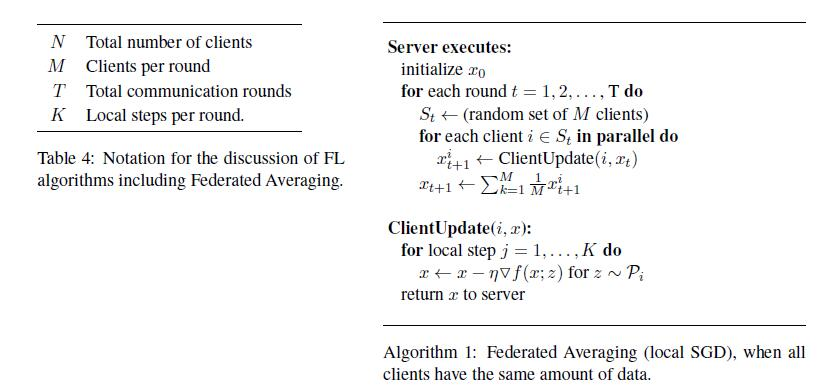
\includegraphics[width=0.9\textwidth]{Federated_Averging.jpg}
    \caption{联邦平均算法}
\end{figure*}

\subsubsection{ IID数据集的优化算法和收敛速度}

虽然可以对正在优化的每个客户端函数进行各种不同的假设, 但最基本的划分是假设IID和非IID数据.在形式上, 在客户端拥有IID数据意味着用于客户端本地更新的每一小批数据在统计上与从整个训练数据集中(客户端所有本地数据集的联合)一致绘制的样本(带有替换)相同.由于客户独立地收集他们自己的培训数据, 这些数据在大小和分布上都有所不同, 而且这些数据不与其他客户或中心节点共享, 因此IID的假设在实践中几乎不可能成立.然而, 这个假设极大地简化了联邦优化算法的理论收敛分析, 并建立了一个基线, 可以用来理解非IID数据对优化率的影响.因此, 自然的第一步是了解IID数据案例的优化算法.

% Communication-Efficient Learning of Deep Networks from Decentralized Data
% \citep{mcmahan2016communication}

% Federated Learning with Non-IID Data 
% \citep{zhao2018federated}
% \section{保护隐私}
 面向隐私保护的机器学习(Privacy-Preserve Machine Learnin, PPML), 指的是使用了保护用户隐私和数据安全的防御技术的机器学习. 其中有以下几种著名方法. \citep{ppmlmancuso}
 \begin{itemize}
     \item 
 安全多方计算(Secure Multiparty Computation,  MPC)
 \item 
 供隐私保护模型训练和预测使用的 同态加密方法(Homomorphic Eneryption,  HE )
 \item 
 用于防止数据泄器的差分隐私 iferntial Piaey, DP) 方法. 
 \end{itemize}
 
 \subsection{隐私保护技术}
 \subsubsection{安全多方计算}
 安全多方计算起初是应对安全两方问题(百万富翁问题).  
  
2.4隐私保护技术
包括三种方法, 分别是安全多方计算、同态加密和差分
本节讨论隐私保护技术, 
隐私. 
2.4.1安全多方计算
安全多方计算最初是针对一个安全两方计算问题, 即所谓的“百万富翁问题”:两个争强好胜的富翁 Alice 和 Bob 在街头相遇, 如何在不暴露各自财富的前提下比较出谁更富有?\citep{scyao1982}

被提出的, 并于1982年由姚期智提出和推广. 在安全多方计算中, 目的是协同地从每一方的隐私输人中计算函数的结果, 而不用将这些输入展示给其他方. 
\paragraph{数学描述}
有 $n $个参与者 $P_1, P_2, ...P_n$, 要以一种安全的方式共同计算一个函数, 这里的安全是指输出结果的正确性和输入信息、输出信息的保密性. 具体地讲, 每个参与者 $P_1$, 有一个自己的保密输入信息 $X_i$, $n $个参与者要共同计算一个函数 $f(X_1, X_2, ... , X_n)=(Y_1, Y_2,  ... , Y_n)$,  计算结束时, 每个参与者 $P_i $只能了解 $Y_i$,  不能了解其他方的任何信息. 

\begin{itemize}
    \item  输入隐私性:安全多方计算研究的是各参与方在协作计算时如何对各方隐私数据进行保护, 重点关注各参与方之间的隐私安全性问题, 即在安全多方计算过程中必须保证各方私密输入独立, 计算时不泄露任何本地数据. 
\item    计算正确性:多方计算参与各方就某一约定计算任务, 通过约定MPC协议进行协同计算, 计算结束后, 各方得到正确的数据反馈. 
    \item     去中心化:传统的分布式计算由中心节点协调各用户的计算进程, 收集各用户的输入信息, 而安全多方计算中, 各参与方地位平等, 不存在任何有特权的参与方或第三方, 提供一种去中心化的计算模式. 
\end{itemize}

\begin{enumerate}
    \item 参与方个数区分
    \item 计算场景区分
\end{enumerate}

主流的两方计算框架的核心是用了混淆电路(Garbled Circuit, 简称GC)和不经意传输(Oblivious Transfer)这两种密码学技术
通用的多方安全计算框架可以让多方安全地计算任何函数或某类函数的结果. 自1986年姚期智提出第一个通用的多方安全计算框架(常被称为Yao’s GC, 即姚氏加密电路)以来, 30多年间已经有BMR、GMW、BGW、SPDZ等多个多方安全计算框架陆续提出. 
\citep{GenExchsecretyao1986}
\paragraph{不经意传输:}
发送方将潜在的许多信息中的一个传递给接收方, 但是对于已传输的信息(如果有的话)则保持忽略. 


\paragraph{n取1 的不经意传输:}设A方有一个输入表 $(x_1..., x_n)$作为输入, 
B方有$i \in 1,  \dots , n$作为输入. n取1的不经意传输是一种安全多方计算协议, 其中
A不能学习到关于$i$的信息, B只能学习到$x_i$
\subsubsection{同态加密}
同态加密指对明文进行环上的加法和乘法运算再加密, 与加密后对密文进行相应的运算, 结果是等价的. 

全同态加密是指同时满足加同态和乘同态性质, 可以进行任意多次加和乘运算的加密函数. 用数学公式来表达, 即$$Dec(f(En(m_1), En(m_2), …, En(m_k)))=f(m_1, m_2, …, m_k)$$, 或写成:$$f(En(m_1), En(m_2), …, En(m_k))=En(f(m_1, m_2, …, m_k))$$, 如果f是任意函数, 称为全同态加密. 
% \cite{encrygoldwass1982}
\paragraph{加法同态}, 如果存在有效算法$\odot$$, E(x+y)=E(x)\odot E(y)$或者$ x+y=D(E(x)\odot E(y))$成立, 并且不泄漏 x 和 y. 
\paragraph{乘法同态}, 如果存在有效算法, $E(x \times y)=E(x) \dot E(y)$或者$ xy=D(E(x) E(y))$成立, 并且不泄漏 x 和 y. 



\subsubsection{差分隐私} 
差分隐私是为了允许研究者在不泄露个体信息(用户隐私)的前提下对一个数据集的整体进行分析而研究出的加密手段. \cite{DPDwork2008}
设想一个受信任的机构持有涉及众多人的敏感个人信息(例如医疗记录、观看记录或电子邮件统计)的数据集, 但想提供一个全局性的统计数据. 这样的系统被称为统计数据库. 但是, 提供有关数据的综合性统计也可能揭示一些涉及个人的信息. 事实上, 当研究人员链接两个或多个分别无害化处理的数据库来识别个人信息时, 各种公共记录匿名化的特殊方法都失效了. 而差分隐私就是为防护这类统计数据库脱匿名技术而形成的一个隐私框架. 

令 $\ varepsilon$ 为正实数, $\mathcal{A}$是将数据集作为输入的随机算法(代表持有数据的受信方的行为). 让 $\textrm{im}\mathcal{A}$表示图像的$\mathcal {A}$. 对于所有数据集$D_{1}, D_{2}$, 
算法$\mathcal{A}$ 提供 $\epsilon-$差分隐私, 在单个元素(即一个人的数据)以及$\mathcal{A}$的所有子集上有所不同 $S$. 
$$ Pr [ \mathcal{A}(D_1) \in S ] \leqslant \exp(\epsilon c) \cdot Pr [ \mathcal{A(D_2)} ] \in S  $$
其中用概率代替算法的随机性.  
  
\paragraph{劣势:}由于对于背景知识的假设过于强(在加噪音的时候需要使用与原数据分布比较类似的噪音函数, 而这一条件就限制了大多数数据其实不满足插分隐私的使用条件), 需要在查询结果中加入大量的随机化, 导致数据的可用性急剧下降. 特别对于那些复杂的查询, 有时候随机化结果几乎掩盖了真实结果. 
\paragraph{应用}
\begin{itemize}
    \item Google的RAPPOR, 用于遥测, 例如了解统计劫持用户设置的恶意软件(RAPPOR's \item open-source implementation)
    \item Google, 分享历史流量统计信息. 
    \item 2016年6月13日, 苹果公司宣布其在iOS 10中使用差异隐私, 以改进其虚拟助理和建议技术,  
    \item 在数据挖掘模型中使用差异隐私的实际表现已有一些初步研究. \citep{FLETCHER201716}
    \item 2020年LinkedIn, 用于广告客户查询
\end{itemize}


% \section{预备知识}

\subsection{再生核希尔伯特空间Reproducing Kernel Hilbert Space}
RKHS由函数构成, 在希尔伯特空间中使用"核技巧"将一组数据映射到一个高维空间, 这个高维空间就是可再生核希尔伯特空间. 

在低维空间中不能线性分割的点集, 通过转化为高维空间中的点集时, 很有可能变为线性可分的.

\paragraph{核方法}
在低维空间中不能线性分割的点集, 通过转化为高维空间中的点集时, 从而变为线性可分的.
\paragraph{核技巧}
在原始空间找到一个函数$K(x_i,x_j)$使得$K(x_i,x_j) = <\phi(x_j),\phi(x_j)>$.
如果这个函数存在, 那么我们只需要在低维空间里计算函数$K(x_i,x_j)$的值即可, 而不需要先把数据映射到高维空间, 再通过复杂的计算求解映射后的内积. 这种简化计算的方法被称为核技巧(The Kernel Trick)

\subsubsection{常用的核函数}

主要有以下几种:

\paragraph{线性核} 其实就是没有映射 $\kappa \left ( x_{1},x_{2} \right ) = \left \langle x{1},x{2} \right \rangle$

\paragraph{高斯核函数}使用最为广泛, 把原始特征映射到无穷维.
 $\kappa \left ( x_{1},x_{2} \right ) = \exp \left ( -\frac{\left | x_{1}-x_{2} \right |^{2}}{2\sigma ^{2}} \right )$

 \paragraph{多项式核函数}, 把数据映射到$C_{n+d}^{n}$维.
$\kappa \left ( x_{1},x_{2} \right ) = \left ( \left \langle x_{1},x_{2} \right \rangle  +R\right )^{d}$

\paragraph{再生核希尔伯特空间}
在一定条件下, 可以找到对应于这个希尔伯特空间上唯一的再生核函数 $K$, 其满足以下几点:\\
对任意固定$x_0$属于$X$, 有$K(x,x_0)$作为$X$的函数属于$H$;\\
对任意$x$属于$X$,$f(.)$ 属于$H$, 有$f(x) = {<f(.),K(.,x)>_{H}}$, 则称$K(.,x)$为$H$的再生核,$H$是以$K(.,x)$为再生核的希尔伯特空间, 简称再生核希尔伯特空间. 

\paragraph{希尔伯特空间定义流程}

向量空间$\rightarrow$内积空间$\rightarrow$赋范向量空间$\rightarrow$度量空间$\rightarrow$Banach空间$\rightarrow$Hilbert空间

\begin{description}
    \item[向量空间Vector Space]:满足加法和标量乘操作的集合
    \item[范数向量空间Normed Vector Space]:定义了向量长度的向量空间$\left || x \right || = <x,x>$
    \item[度量空间Metric Space]:定义了两个点的距离的集合
    \item[巴拿赫空间Banach Space]:一个完备的范数向量空间
    \item[内积空间Inner Product Space]:指在定义域上可进行内积运算法操作的向量空间
    \item[希尔伯特空间Hilbert Space]:当一个内积空间满足通过内积空间可推导出范数空间, 且是完备的, 那么这个内积空间就是希尔伯特空间. 

\end{description}
\paragraph{RKHS的两个定理}
\begin{itemize}
    \item 
    一个希尔伯特空间H是一个再生核希尔伯特空间, 当且仅当它有一个再生核
    \item 
    对于给定的再生核希尔伯特空间, 其再生核是唯一的. 
\end{itemize}


\paragraph{经典RKHSs技术的三个问题} \cite{peifer2020sparse}
 \begin{itemize}
     \item 首先, 它们需要先验知识, 而这在许多应用中是不现实的.此外, RKHS的选择会影响溶液的形状和平滑度, 从而影响其性能.
     \item其次, RKHS不具备处理异构平滑度的能力, 也就是说, 函数在其领域的某些部分是平滑的, 但在其他部分变化迅速.
     \item最后, 随着训练样本中数据点的增加, 评估这些方法解的计算复杂度增加, 使得这些技术在许多应用中不可行.
    
 \end{itemize}
 虽然核学习、局部核自适应和稀疏性已被用于解决这些问题, 但这些方法中的许多都是计算密集型的或放弃了最优性保证.
 可以利用RKHSs中的一个新的积分表示来解决这些问题, 这些RKHSs允许任意中心和每个中心的不同内核.为了解决复杂性问题, 我们然后将函数估计问题写成一个稀疏函数程序, 它显式地最小化导致低复杂性解决方案的表示法的支持.尽管这些问题具有非凸性和无限维数, 但我们证明利用对偶性可以准确有效地解决这些问题, 并在模拟和实际数据中说明了这种新方法.
%% 这儿总结一些比较重要的数学概念、定理等.
\subsection{梯度下降}
\subsubsection{随机梯度下降Stochastic gradient descent}
随机梯度下降(通常缩写SGD)是一种迭代方法用于优化的目标函数与合适的光滑性质(例如可分化或subdifferentiable).它可以被看作是随机逼近的梯度下降优化, 因为它取代了实际梯度(从整个计算数据集通过其估计值(从数据中随机选择的子集计算)).特别是在大数据应用中, 这减轻了计算负担, 实现更快的交易迭代, 但收敛速度略低. 
\begin{algorithm}  
    \caption{ Stochastic  General decent method}  
    \begin{algorithmic}
\STATE{ Choose an initial vector of parameters  w and learning rate  $\eta$ .Repeat until an approximate minimum is obtained:
\begin{itemize}
    \item Randomly shuffle examples in the training set.
    \item For $  i=1, 2, ..., n$,  do:
    $w:=w-\eta \nabla Q_{i}(w)$ 
\end{itemize}
}
    \end{algorithmic}  
   \end{algorithm}  
\subsubsection{ADMM 交替向量乘子法}
ADMM也是增广拉格朗日函数, 只是由一个变量变成两个变量
$$L(x, z;\lambda)= f(x) + g(z) + \lambda ^T(Ax + Bz - c) + \rho/2 * ||Ax + Bz -c ||^2$$
固定其中两个变量, 去更新第三个变量的值

$ \text{step1}: x^{k+1} = arg \min_x L(x, z^k, \lambda^k) \\
\text{step2}: z^{k+1} = arg min_z L(x^{k+1}, z, lambda^k) \\
\text{step3}: \lambda ^ {k+1} = \lambda^k + \rho (Ax + Bz - c) \\$
于是问题就变化为了如何求解 $arg min_x L$
\subsubsection*{decentralized SGD去中心化 SGD}
 

Decentralized Federated Learning via SGD over Wireless D2D Networks (H Xing,  O Simeone,  S Bi)

\subsection{张量分解}
张量(tensor)是一个多维的数据存储形式, 数据的的维度被称为张量的阶.它可以看成是向量和矩阵在多维空间中的推广, 向量可以看成是一维张量, 矩阵可以看成是两维的张量.
\subsubsection{CP分解}
将高维的张量分解成为Rank-One Tensors的和.
$X \approx [ \!  [ \mathbf{A, B, C} ]\!] \equiv \sum_{r=1}^{R}a_r \circ b_r \circ c_r$

这里$\circ$指的是外积.
\subsubsection{Tucker 分解  }

Tucker分解将张量分解为一组矩阵和一个小的核心张量.

 $X = G \times_1 A^{(1)} \times_2  A^{(2)} \dots \times_N A^{(N)}= [\! [  G:A^{(1)},  A^{(2)},  A^{(N)}   ] \! ] $

\subsection{Dataset shift 数据集偏移}
数据集偏移是指训练和测试分布不同时的情况.
数据集偏移主要发生在有监督的机器学习范式和半监督学习的混合范式内.
数据集移位的问题可能源于利用输入特征的方式, 选择训练和测试集的方式, 数据稀疏性, 由于非平稳环境而导致的数据分布移位, 以及源于各层内激活模式的变化.深度神经网络.
数据集移位的表现形式:协变量移位、先验概率转移、概念转变、内部协变量移位(协变量移位的重要子类型)

\subsubsection{有状态和无状态}
有状态就是有数据存储功能.有状态对象(Stateful Bean), 就是有实例变量的对象 , 可以保存数据, 是非线程安全的.在不同方法调用间不保留任何状态.

无状态就是一次操作, 不能保存数据.无状态对象(Stateless Bean), 就是没有实例变量的对象.不能保存数据, 是不变类, 是线程安全的.
 
\subsection{激活函数}
激活函数在神经元中非常重要的.为了增强网络的表示能力和学习能力, 激活函数需要具备以下几点性质:
\begin{enumerate}
\item 连续并可导(允许少数点上不可导)的非线性函数.可导的激活函数可以直接利用数值优化的方法来学习网络参数.
\item 激活函数及其导函数要尽可能的简单, 有利于提高网络计算效率.
\item 激活函数的导函数的值域要在一个合适的区间内, 不能太大也不能太小, 否则会影响训练的效率和稳定性.
\end{enumerate}
\subsubsection{Sigmoid型函数}
常用的Sigmoid 型函数有Logistic 函数和Tanh 函数.
\paragraph{Logistic函数}
$$\sigma(x)=\frac{1}{1+\exp(-x)}$$
和感知器使用的阶跃激活函数相比, Logistic 函数是连续可导的, 
装备了Logistic激活函数的神经元具有以下性质:
\begin{enumerate}
    \renewcommand{\labelenumi}{(\theenumi)}
 \item 其输出直接可以看作概率分布, 使得神经网络可以更好地和统计学习模型进行结合. 
 \item 其可以看作一个软性门(Soft Gate), 用来控制其他神经元输出信息的数量.
\end{enumerate}

\textbf{优点}:
\begin{enumerate}
    \renewcommand{\labelenumi}{(\theenumi)}
\item 便于求导的平滑函数;
\item 能压缩数据, 保证数据幅度不会有问题;
\item 适合用于前向传播.
\end{enumerate}

\textbf{缺点}:
\begin{enumerate}
    \renewcommand{\labelenumi}{(\theenumi)}
    \item 容易出现梯度消失的现象 
   \item Sigmoid的输出不是0均值 的:这会导致后层的神经元的输入是非0均值的信号, 这会对梯度产生影响.以 $f=\mathrm{sigmoid}(wx+b)$为例,  假设输入均为正数(或负数), 那么对w的导数总是正数(或负数), 这样在反向传播过程中要么都往正方向更新, 要么都往负方向更新, 导致有一种捆绑效果, 使得收敛缓慢.
    \item 幂运算相对耗时 
\end{enumerate}
\paragraph{求导}
$ \frac{\rho \sigma(x)}{\rho(x)}=\sigma(x)(1-\sigma(x))$
​	 
\paragraph{Tanh函数}
$$\tanh(x)=\frac{\exp(x)-\exp(-x)}{\exp(x)+\exp(-x)} $$
Tanh 函数可以看作放大并平移的Logistic 函数, 其值域是(-1,  1).
$$\tanh(x) = 2 \sigma (2x)-1$$

\begin{figure}[!ht]
    \centering
    % \label{ }
    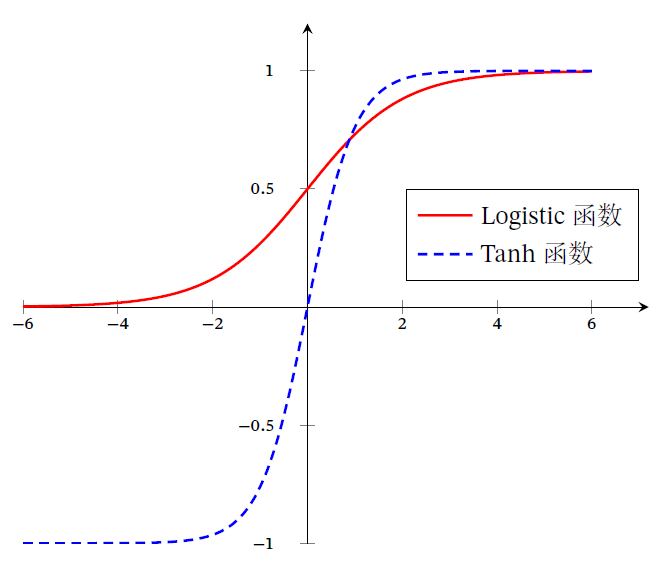
\includegraphics[width=0.4\textwidth]{sigmoid_function.png}
    \caption{Logistic 函数和Tanh 函数}
\end{figure}

\textbf{优缺点}:
Tanh函数是0均值的, 解决了Sigmoid函数的非zero-centered问题, 但是它也存在梯度消失和幂运算的问题.


\subsubsection{整流线性单位函数(Rectified Linear Unit,  ReLU)}
ReLU 实际上是一个斜坡(ramp)函数, 定义为
$$\mathrm{ReLU}(x)=
\left\{ 
\begin{array}{c}    x \\    0  \\   \end{array}
\right. =\max(0, x)
$$
\begin{figure}[!ht]
    \centering
    \includegraphics[width=\textwidth]{ReLU}
    \caption{ReLU激活函数}
\end{figure}
\paragraph{求导}
$$\frac{\rho\sigma(x)}{\rho(x)}=1-\sigma^2(x)$$

\textbf{优点}:
\begin{enumerate}
    \renewcommand{\labelenumi}{(\theenumi)}
    \item   ReLu的收敛速度比 sigmoid 和 tanh 快(梯度不会饱和, 解决了梯度消失问题);
     \item  计算复杂度低, 不需要进行指数运算;
     \item 适合用于后向传播.
\end{enumerate}

\textbf{缺点}:
\begin{enumerate} 
    \renewcommand{\labelenumi}{(\theenumi)}
\item  ReLU的输出不是zero-centered; 
\item  Dead ReLU Problem(神经元坏死现象):某些神经元可能永远不会被激活, 导致相应参数永远不会被更新(在负数部分, 梯度为0).

\textbf{产生原因}:
\begin{itemize}
    \item 参数初始化问题
    \item 学习率太高导致在训练过程中参数更新太大
\end{itemize}
 \textbf{解决方法}:采用Xavier初始化方法, 以及避免将学习率设置太大或使用adagrad等自动调节学习率的算法.
\item ReLU不会对数据做幅度压缩, 所以数据的幅度会随着模型层数的增加不断扩张.
\end{enumerate}
\paragraph{Leakly  ReLU函数}
用来解决ReLU带来的神经元坏死的问题, 可以将0.01设置成一个变量a, 其中a由后向传播学出来.但是其表现并不一定比ReLU好.

\begin{align*}
\mathrm{ELU}(x)=&
\left\{ 
\begin{array}{c c}    
    x  \ & \text{if} \  x>0 \\    
    \gamma_i x \ & \text{if} \ x \leqslant 0  \\   
\end{array} 
\right. \\
=& \max(0, x)+\gamma_i \min(0, x)
\end{align*}
其中$\gamma_i$为$x \leqslant 0 $时函数的斜率

\paragraph{ELU函数(指数线性函数)}
ELU有ReLU的所有优点, 并且解决了 Dead ReLU问题, 输出的均值接近0(zero-centered).但是计算量大, 其表现并不一定比ReLU好.
\begin{align*}
    \mathrm{ELU}(x)= &
    \left\{ 
    \begin{array}{c c}    
        x  \ & \text{if} \  x>0 \\    
        \gamma(\exp(x)-1) \ & \text{if} \ x \leqslant 0  \\   
    \end{array} 
    \right. \\
    = & \max(0, x)+\gamma_i \min(0, \gamma(\exp(x))-1)
    \end{align*}
      

\subsubsection{Entropy熵}
在信息论中, 熵用来衡量一个随机事件的不确定性.
 自信息(Self Information)表示一个随 机事件所包含的信息量. 一个随机事件发生的概率越高, 其自信息越低.如果-一个事件必然发生, 其自信息为0.
 对于一一个随机变量X (取值集合为X , 概率分布为$p(x,  x \in \mathcal{X})$, 当X=x
 时的自信息$I(x)$定义为
 \begin{equation}
      I(x)=- \log p(x).
 \end{equation} 
 
 在自信息的定义中, 对数的底可以使用2、自然常数$e$或是10.当底为2时, 自信息的单位为bit;当底为e时, 自信息的单位为nat.
 对于分布为$p(x)$的随机变量X , 其自信息的数学期望, 即熵$H(X)$定义为
 
 \begin{equation}
    \begin{split}
 H(X) &= \mathbb{E}_x\left[  I(x)\right] \\
 &= \mathbb{E}_x \left[  -\log p(x) \right] \\
 &=\sum_{x \in \mathcal{X}}p(x) \log p(x)    
\end{split}
 \end{equation}
 其中$ 0 \log 0= 0 $.
 熵越高, 则随机变量的信息越多;熵越低, 则随机变量的信息越少

\subsubsection{Cross Entropy交叉熵}
对于分布为$p(x)$的随机变量, 熵$H(p)$表示其最优编码长度.交叉熵(Cross Entropy)是按照概率分布$q$的最优编码对真实分布为$p$的信息进行编码的长度, 定义为 
\begin{equation}
 \begin{split}
        H(p, q)&= \mathbb{E}_p \left[ -\log q(x) \right]  \\
        &= - \sum_x p(x) \log q(x) 
 \end{split}
\end{equation}
 
在给定$p$的情况下, 如果$q$ 和$p$ 越接近, 交叉熵越小;如果$q$ 和$p$ 越远, 交叉熵就越大.


\subsection{神经网络}
“神经网络是由具有适应性的简单单元组成的广泛并行互连的网络, 它的组织能够模拟生物神经系统对真实世界物体所作出的交互反应”[Kohonen,  1988].

神经网络中最基本的单元是神经元模型(neuron), 最简单的神经元模型是“M-P神经元模型”.
树突对应于输入部分, 每个神经元收到n个其他神经元传递过来的输入信号, 这些信号通过带权重的连接传递给细胞体.
细胞体分为两部分, 前一部分计算总输入值(即输入信号的加权和), 后一部分先计算总输入值与该神经元阈值的差值, 然后通过激活函数的处理, 产生输出从轴突传送给其它神经元.
\begin{figure}
    \centering
    \label{MP_Model}
    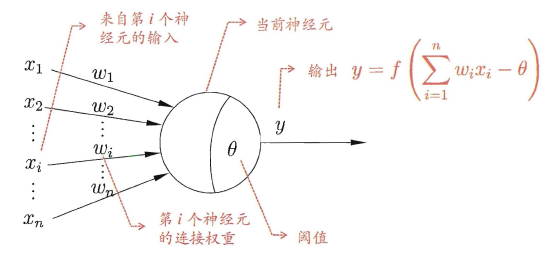
\includegraphics[width=0.9\textwidth]{MP_Modle.png}
    \caption{M-P神经元模型}
\end{figure}

神经元模型最理想的激活函数也是阶跃函数, 但阶跃函数不连续, 常采用Sigmoid函数来近似.

\subsubsection{感知器}
感知机(Perceptron)是由两层神经元组成的一个简单模型, 但只有输出层是M-P神经元, 即只有输出层神经元进行激活函数处理, 也称为功能神经元;输入层只是接受外界信号(样本属性)并传递给输出层(输入层的神经元个数等于样本的属性数目), 而没有激活函数感知机的输出层应该可以有多个神经元, 从而可以实现多分类问题, 同时两个模型所用的参数估计方法十分不同.

\begin{figure}
    \centering
    \label{MP}
    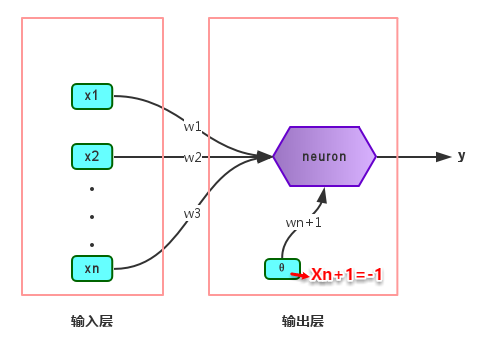
\includegraphics[width=0.5\textwidth]{simple_perceptron.png}
    \caption{简单感知机}
\end{figure}
\newpage
\paragraph{感知机学习算法} 给定个样本的训练集${(x^{(n)}, y^{(n)}}^N_{n1}$, 其中$y(n)\in {+1, -1}$, 感知器学习算法试图找到一组参数$\mathbf{w}^{\star}$, 使得对于每个样本$(x^{(n)}, y^{(n)}$有
\begin{equation}
    y^{(n)} \mathbf{w}^{\star \mathrm{T} }  \mathcal{x}^{(n)}> 0,  \forall n \in \{ 1, ..., N \}
\end{equation}
\begin{figure}
    \centering
    \label{algorithm_perceptron}
    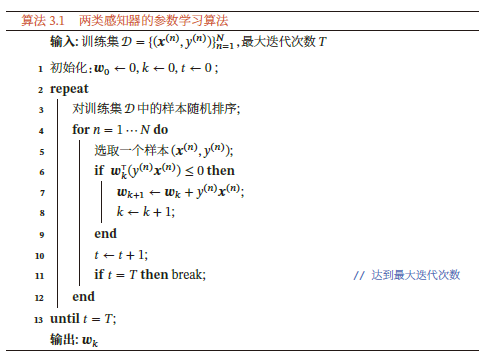
\includegraphics[width=0.9\textwidth]{algorithm_perceptron.png}
    \caption{两类感知机学习算法 }
\end{figure}

\paragraph{感知器的收敛性} 
 感知器收敛性:给定训练集 $D = {x(), y(0)}$令R是训练集
中最大的特征向量的模, 即$$R = \max_n \|x^{(n)}\|$$
如果训练集D线性可分, 两类感知器的参数学习算法3.1的权重更新次数不
超过$\frac{R^2}{\gamma^2}$次.

\paragraph{几种常见的线性模型对比} 
\begin{figure}
    \centering
    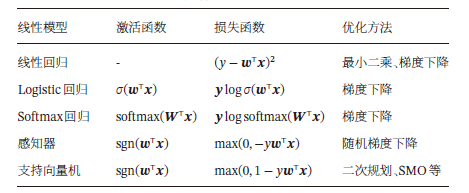
\includegraphics[width=0.7\textwidth]{linear_model.png}
    
\end{figure}
\newpage
\paragraph{不同损失函数的比较}
\begin{figure}
    \centering
    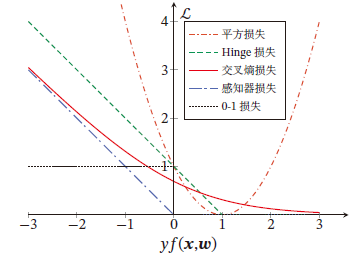
\includegraphics[width=0.7\textwidth]{loss_function.png}
    \caption{不同损失函数的比较}
\end{figure} 
一个好的损失函数应该随着$yf(\mathbf{x;w})$的增大而减少.

\subsubsection{分类问题总结}
分类问题中的决策函数需要输出离散值或是标签的后验概率.线性分类模型一般是一
个广义线性函数, 即一个或多个线性判别函数加上一个非线性激活函数.在Logistic 回归和Softmax 回归中, y 为类别的one-hot 向量表示;在感知器和支持向量机中, y 为$\{+1, -1\}$.



\subsubsection{数据集}
如果已经有了一个比较大的标注数据集, 想要完成一个有监督模型的测试, 那么通常使用均匀随机抽样的方式, 将数据集划分为训练集、验证集、测试集, 这三个集合不能有交集, 常见的比例是8:1:1. 三个集合都是同分布的. 
训练集就是用来训练参数的. 而验证集基本是在每次epoch完成后, 测试当前模型的准确率. 
对于一个模型来说, 其参数可以分为普通参数和超参数. 除强化学习外, 普通参数是可以被训练所更新. 超参数不在梯度下降的更新范围内, 需要人工根据验证集调节.所以在广义上, 验证集参与了人工调参的过程, 需要一个没有经过的训练的集合, 就是测试集来测试最终准确率. \citep{training_validation_test_Su}


\subsection{前馈神经网络}
在前馈神经网络中, 不同的神经元属于不同的层, 每一层的神经元可以接受到前一层的神经元信号, 并产生信号输出到下一层.第0层叫做输入层, 最后一层叫做输出层, 中间的叫做隐藏层, 整个网络中无反馈, 信号从输入层到输出层单向传播, 可用一个有用无环图表示.

前馈神经网络也成为多层感知器(Mutlti-Layer Perceptron, MLP).但是这种叫法并不准确, 因为前馈神经网络其实是由多层Logistic回归模型(连续的非线性模型)组成, 而不是有多层感知器模型(非连续的非线性模型)组成.

下图为简单的前馈神经网络图:

\begin{figure}[!ht]
    \centering
    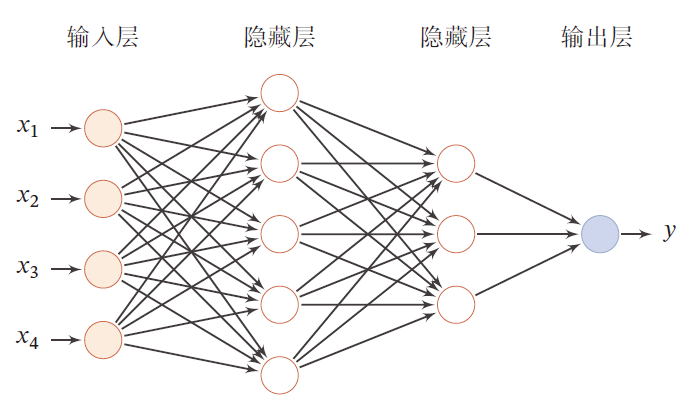
\includegraphics[width=0.6\textwidth]{FNN}
    \caption{前馈神经网络图}
\end{figure} 


神经网络中涉及的多个记号:
\begin{table}[!ht]
    \renewcommand{\arraystretch}{1.35}  
    \centering
    \begin{tabular}{cc}
        \toprule
        记号 & 含义 \\
        \midrule
        $L$ &表示神经网络的层数\\
$m^{(l)}$&表示第$ l$ 层神经元个数\\
$f_l ( \cdot ) $&表示第$ l $层神经元的激活函数\\
$W^{(l)}$   &表示第$ l-1$ 层到第 l 层的权重矩阵\\
$b^{(l)}$   &表示第$ l-1$ 层到第 l 层的偏置\\
$z^{(l)}$   &表示第 $l$ 层神经元的净输入(净活性值)\\
$a^{(l)}$   &表示第$l$层的神经元输出(活性值)\\
        \bottomrule
    \end{tabular}
\label{tabel:NerualNetwork_mark}
\caption{神经网络中涉及的记号}
\end{table}

神经网络的信息传播公式如下 
\begin{gather*}
 z^{(l)} = W^{(l)}   a^{(l-1)} + b^{(l)}\\
 a^{(l)} = f_l(z^{(l)})
\end{gather*} 
 可以合并写为 :
$$z^{(l)}=W^{(l)} f_{(l-1)} (z^{(l-1)})+b^{^{(l)}}  $$
或者 
$$a^{(l)} = f_l(W^{(l)} a^{(l-1)} + b^{(l)})$$
这样神经网络可以通过逐层的信息传递, 得到网络最后的输出$a^{(l)}$.整个网络可以看做一个符合函数$$\phi (x; W, b)$$
将向量x作为第一层的输入$a^0$, 将第 l 层的输入$a^0$,  将第L层的输出$a^{(l)}$ 作为整个函数的输出.
$$ x = a^0 \rightarrow z^1 \rightarrow a^1 \rightarrow z^2 .... \rightarrow a^{L-1} \rightarrow z^{(l)} \rightarrow a^{(l)} = \phi (x;W, b)$$
其中W,  b表示网络中所有层的连接权重和偏置. 
\paragraph{参数学习}
如果采用交叉熵损失函数, 对于样本$(x, y)$, 其损失函数为:
$$L(y, \hat{y}) = -y^T log (\hat{y})$$, 
其中 y 属于${0, 1}^T$为标签y对应的one-hot向量.

给定训练集$D={(x^{(n)}, y^{(n)},  N>=n>=0}$, 将每个样本$x^n$ 输入给前馈神经网络, 得到网络输出为$y^n$, 其在数据集$\mathcal{D}$上的结构化风险函数为:
$$R(W, b)=\frac{1}{N}\sum_{n=1}^{N} L(y^n, \hat{y}^n) + \frac{1}{2}\lambda \left \| W \right \|_F^2$$
 
其中W和b分别表示网络中所有的权重矩阵和偏置向量,  $\|W\|_F^2$ 是正则化项, 用来防止过拟合, $\lambda$是为正数的超参数, $\lambda$越大, W越接近于0.这里的$(\|W\|_F)^2$一般使用Frobenius范数.
 
有了学习准则和训练样本, 网络参数可以通过梯度下降法来进行学习.在梯度下降方法的每次迭代过程中, 第l层的参数$ W^{(l)} $和$ b^{(l)}$ 参数更新方式为:
\begin{gather*}
    W^{(l)} \leftarrow W^{(l)} - \alpha \frac{\partial R(W, b)}{\partial W^{(l)}}=W^{(l)} - \alpha ( \frac{1}{N} \sum_{n=1}^{N}(\frac{\partial L(y^n, \hat{y}^n)}{\partial W^{(l)}}) + \lambda W^{(l)} )\\b^{(l)} \leftarrow b^{(l)} - \alpha \frac{\partial R(W, b)}{\partial b^{(l)}}=b^{(l)} - \alpha ( \frac{1}{N} \sum_{n=1}^{N}(\frac{\partial L(y^n, \hat{y}^n)}{\partial b^{(l)}}) ) 
\end{gather*}
其中$\alpha$为学习率.
梯度下降法需要计算损失函数对参数的偏导数, 如果通过链式法则逐一对每个参数进行求偏导效率比较低.在神经网络的训练中经常使用反向传播算法来高效的计算梯度. 
\subsubsection{反向传播算法}
基于误差的反向传播算法(backpropagation, BP)的前馈神经网络训练过程可以分为以下三步:
\begin{enumerate} 
    \renewcommand{\labelenumi}{(\theenumi)}
\item 前馈计算每一层的净输入$z^{(l)}$ 和激活值 $a^{(l)}$, 直到最后一层
\item 反向传播计算每一层的误差项
\item 计算每一层参数的偏导数, 并更新参数
\end{enumerate}

它利用均方误差和梯度下降的方法来实现对网络连接权值的修改.网络连接权值的修改是为了使误差平方和最小.该算法首先对网络的连接值赋一个小的值, 然后选择一个训练样本来计算相对于这个样本的误差梯度.
\begin{figure}
    \centering
    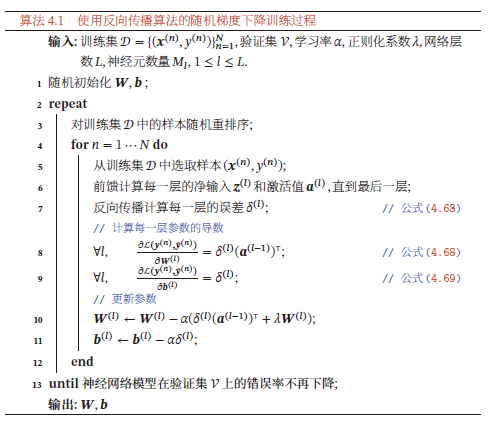
\includegraphics[width=0.7\textwidth]{algorithm_bp.png}
\end{figure} 

\subsubsection{优化问题}
\paragraph{非凸优化问题}
使用非凸的损失函数
如平方误差损失函数和交叉熵损失函数
\paragraph{梯度消失问题}
由于Sigmoid 型函数的饱和性, 饱和区的导数更是接近于0.这样, 误差经
过每一层传递都会不断衰减.当网络层数很深时, 梯度就会不停衰减, 甚至消
失, 使得整个网络很难训练.这就是所谓的梯度消失问题(Vanishing Gradient
Problem), 也称为梯度弥散问题.

\subsubsection{通用近似定理}
通用近似定理( Universal Approximation Theorem) 

令$\Phi(\cdot)$是一个非常数、有界、单调递增的连续函数,  $\mathcal{J}_D$是一个D维的单位超立方体$[0, 1]^D$,  $C(\mathcal{p})$是定义在$\mathcal{J}_D$.上的连续函数集合对于任何-一个函数$f \in C(\mathcal{J}_D)$, 存在一个整数M, 和一组实数$v_m, b_m \in R$以及实数向量$v_m \in R^D, m= 1,  \cdots,  M$ 以至于我们可以定义函数
$$F(x) =2v_m \phi(v_m^T x + b_m)$$
作为函数f的近似实现, 即
$$|F(x)- f(x)|< \upsilon_i \forall x \in (\mathcal{J}_D) $$
其中$ \upsilon > 0$是一个很小的正数.


一个前馈神经网络如果具有线性输出层和至少一层具有任何一种"挤压"性质的激活函数(例如 sigmoid激活函数)的隐藏层, 只要给予网络足够数量的隐藏单元, 它可以以任意的精度来近似任何一个任何定义在实数空间$ R^D$中的有界闭集函数(Borel 函数). 神经网络的通用近似性质也被证明对于其他类型的激活函数, 比如ReLU, 也都是适用的.

学习失败原因:
\begin{itemize}
    \item 用于训练的优化算法可能找不到用于期望函数的参数值.
    \item 训练算法可能由于过拟合而选择了错误的函数.
\end{itemize}
\subsection{循环神经网络}

\textbf{前馈网络的一些不足}
\begin{itemize}
    \item 连接存在层与层之间, 每层的节点之间是无连接的(无循环)
    \item 输入和输出的维数都是固定的, 不能任意改变.无法处理变长的序列数据.
    \item 假设每次输入都是独立的, 也就是说每次网络的输出只依赖于当前的输入.
\end{itemize}

\textbf{循环神经网络}(Recurrent Neural Network, RNN)通过使用带自反馈的神经元, 能够处理任意长度的序列, 比前馈神经网络更加符合生物神经网络的结构.
给定-一个输入序列$x_{1:T} =(x_1, x_2,  .... x_t, .... x_T)$, 循环神经网络通过下面公式更新带反馈边的隐藏层的活性值$h_t$:
$$h_t= f(h_t-1, x_t)$$
其中$h_0= 0, f( \cdot )$为一个非线性函数, 可以是一个前馈网络.
\begin{figure}[!htb]
    \center
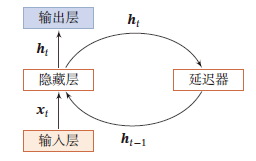
\includegraphics[width=0.7\textwidth]{RNN_sample.png}
\caption{循环神经网络}
\end{figure}


图中“延时器”为一个虚拟单元, 记录神经元的最近一次(或几次)活性值.
\subsubsection{简单循环网络}
Simple Recurrent Network, SRN \citep{elman1990finding} 
 
$$h_t = f(Uh_t-1 +Wx_t + b)$$
\begin{figure}[!htb]
    \center
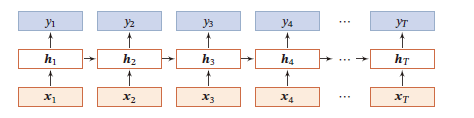
\includegraphics[width=0.7\textwidth]{simple_RNN.png}
\caption{按时间展开的循环神经网络}
\end{figure}


\subsubsection{循环神经网络的计算能力}
循环神经网络的拟合能力十分强大.一个完全连接的循环网络是任何非线性动力系统的近似器.
如果一个完全连接的循环神经网络有足够数量的sigmoid 型隐藏神经元, 它可以以任意的准确率去近似任何一个非线性动力系统

\begin{equation*}
    \begin{split}
        S_t &= g(S_{t-1}, x_t) \\
        y_i & = o(s_t)
    \end{split}
\end{equation*}
其中$S_t$为每个时刻的隐状态, $x_t$是外部输入, $g(\cdot)$是可测的状态转换函数, 
$o(\cdot)$ 是连续输出函数, 并且对状态空间的紧致性没有限制.
 
\begin{figure}[!htb]
    \center
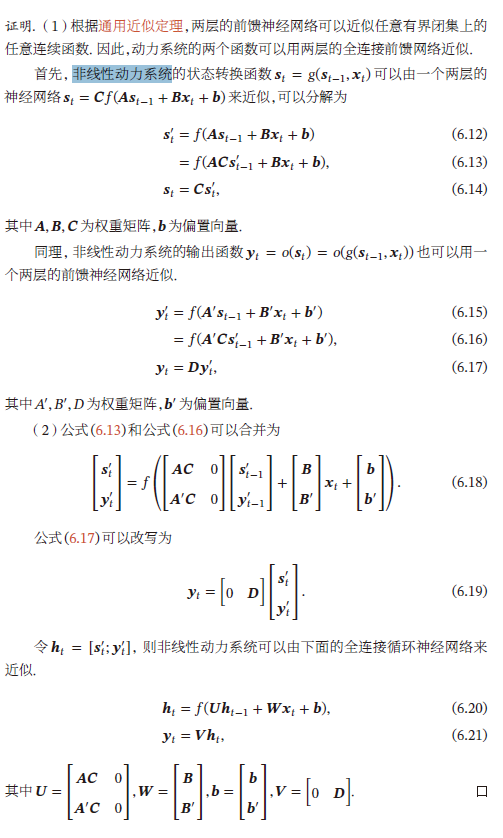
\includegraphics[width=0.8\textwidth]{RNN_univesal.png}
\end{figure}



% \subsubsection{循环神经网络在机器学习中的应用}


 \paragraph{长期依赖(Long-Term Dependencies)问题}
如果相关信息和当前预测位置之间的间隔就相当的大, 在这个间隔不断增大时,  RNN会难以学习到连接如此远的信息. (梯度消失和梯度爆炸)

在序列中, 依赖现象较为明显, 如主谓依赖、名词与动词单复数的依赖. 在较短范围内, 这种依赖能够被传统的语言模型(如n-gram, 神经语言模型)刻画, 但是长距离依赖则是传统语言模型难以刻画的. 长距离依赖是序列建模的重要刻画内容之一.
循环神经网络在进行梯度反向传播时也面临着梯度消失和梯度爆炸问题, 只是表现在时间轴上, 即如果输入序列很长,  梯度难以更新. 



解决: LSTM GRU Attention


\paragraph{序列到类别模式}

输入为序列, 输出为类别.比如在文本分类中, 输入数据为单词的序列, 输出为该文本的类别.

假设一个样本$$ x_{1:T}=(x_1, ...,  x_T)$$ 为一个长度为T的序列, 输出为一个类别 $y \in {1,  2,  \dot C}$.可以将样本x按不同时刻输入到RNN中, 得到不同时刻的隐藏状态 $h_1,  \dots,  h_T$ .可以将 $h_T$看作整个序列的最终表示, 并输入给分类器 $g(\cdot)$进行分类,  $\hat{y}=g(h_T)$

其中 $g(\cdot)$可以是简单的线性分类器如Logistic回归, 或复杂分类器如前馈神经网络.

除了将最后时刻的状态作为小于列表示之外, 还可以对整个序列的所有状态进行平均, 用这个平均状态作为整个序列的表示:
\begin{figure}[!htb]
    \center
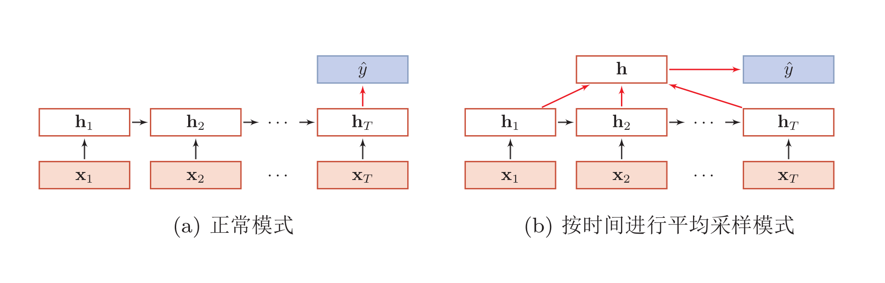
\includegraphics[width=0.8\textwidth]{RNN_model1.png}
\caption{序列到类别模式}
\end{figure}


\paragraph{同步的序列到序列模式}

\begin{figure}[!htb]
    \center
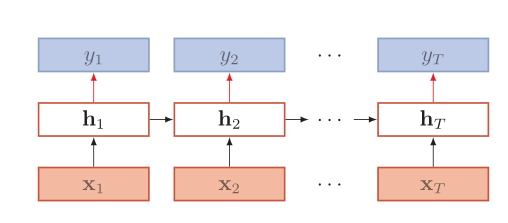
\includegraphics[width=0.8\textwidth]{RNN_model2.png}
\caption{同步的序列到序列模式}
\end{figure}
每一时刻都有输入和输出, 输入序列和输出序列的长度相同, 如词性标注(Part-of-Speech Tagging)中, 每一个单词都需要标注其对应的词性标签.

输入为一个长度为T的序列$$ x_{1:T}=(x_1, ...,  x_T)$$, 输出为序列$y_{1:T}=(y_1, ...,  y_T)$.样本x按不同时刻输入到RNN中, 并得到不同时刻的隐状态$h_1,  \dots,  h_T$ .每个时刻的隐状态$h_t$代表了当前时刻和历史的信息, 并输入给分类器 $g(\cdot)$得到当前时刻的标签 $ \hat{y}_t$ .
$$\hat{y}= g(h_t),  \  \forall t \in [1, T]$$



\paragraph{异步的序列到序列模式}
也称为编码器-解码器(Encoder-Decoder)模型, 输入序列和输出序列不需要严格的对应关系, 也不需要保持相同的长度.类似于机器翻译.

输入为一个长度为T的序列 $ x_{1:T}=(x_1, ...,  x_T)$, 输出长度为M的序列 $ y_{1:T}=(y_1, ...,  y_T)$ .先将样本x按不同时刻输入到RNN中(编码器), 得到其编码 $h_T$ , 然后使用另一个RNN(解码器), 得到输出序列$ \hat{y}_{1:m}$ , 为了建立输出序列之间的依赖关系, 在解码器中通常使用非线性的自回归模型.

\begin{equation}
    \begin{split}
        h_t &= f_1(hp_1, x),   \forall t \in [1, T] \\
    h_{T+t}& = f_2(h_{T+t-1}, \hat{y}_{t-1}),  \forall t\in[1, M]\\
    \hat{y}&= g(h_{T+t}),   \forall t\in[1, M]
    \end{split} 
\end{equation}

其中 $f(\cdot)$ 为编码器和解码器的神经网络,  $g(\cdot)$ 为分类器,  $\hat{Y}_t$为预测输出 $\hat{y}_t$的向量表示.
\begin{figure}[!htb]
    \center
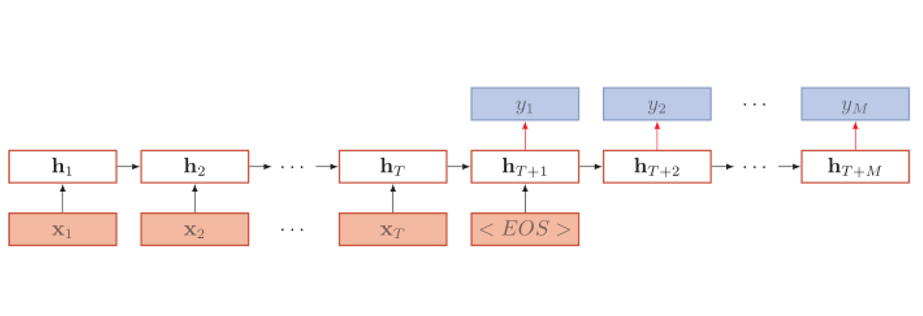
\includegraphics[width=0.8\textwidth]{RNN_model3.png}
\caption{异步的序列到序列模式}
\end{figure}

% \subsubsection{========}

% 将字符打乱顺序普通神经网络无法预测下一个

% \begin{tikzcd}
%     &  \arrow[rd,  "\mathbf{b}^{(l)} \to \mathbf{I}_{m^{(l)}}"] &                                      &                                         & {\partial{L}(\mathbf{y},  \hat{\mathbf{y}})} \arrow[lld,  "\delta^{l}"'] \arrow[d,  "\delta^{l+1}"] &  \\
% \mathbf{a}^{(l-1)} \arrow[rr,  "W_{ij}^{(l)} \to a_{j}^{(l-1)}"'] &                                                          & \sum \mathbf{z}^{(l)} \arrow[r,  "f"] & \mathbf{a}^{(l)} \arrow[r,  "W^{(l+1)}"] & \mathbf{z}^{(l+1)} \arrow[r,  "f"]                                                                &  \\
%     &  \arrow[ru]                                              &                                      &                                         &                                                                             & 
% \end{tikzcd}


% \textbf{RNN应用在知识图谱--图网络}

\subsubsection{简介实现}

\begin{enumerate}
    \item  使用困惑度评价模型. 
    \item  在迭代模型参数前裁剪梯度. 
    \item  对时序数据采用不同采样方法将导致隐藏状态初始化的不同
\end{enumerate}

\subsection{通过时间反向传播}
BPTT 算法将循环神经网络看作一个展开的多层前馈网络, 其中“每一层”对应循环网络中的“每个时刻”, 所有层的参数是共享的, 因此参数的真实梯度是所有“展开层”的参数梯度之和.
% \begin{figure}[!htb]
%     \center
% 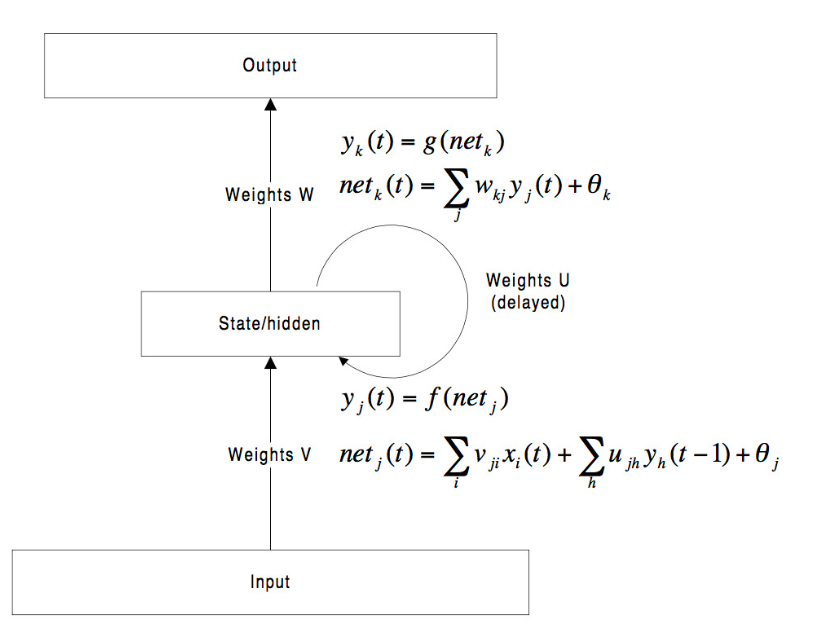
\includegraphics[width=0.6\textwidth]{BPTT.png}
% \caption{BPTT算法}
% \end{figure}
假设
\begin{itemize}
\item 激活函数$\Phi(x)=x$, 
\item t时刻输入$\mathbf{x}_t \in \mathbb{R}^d$, 
\item 标签 $y_t$
\item 隐藏状态 $\mathbf{h}_t \in \mathbb{R}^h$
\item 隐藏层权重 
$$\mathbf{W}_{hx} \in \mathbb{R}^{h \times d}$$
$$\mathbf{W}_{hh} \in \mathbb{R}^{h \times h}$$
\item 输出层权重
$\mathbf{W}_{qh} \in \mathbb{R}^{q \times h}$
\item
t时刻输出$\mathbf{o}_t \in \mathbb{R}^q$, 

$$\mathbf{o}_t = \mathbf{W}_{qh} \mathbf{h}_{t}.$$
\item 
t 时刻损失 $\ell(\mathbf{o}_t,  y_t)$
时间步数为T的损失函数$$L = \frac{1}{T} \sum_{t=1}^T \ell (\mathbf{o}_t,  y_t).$$
\end{itemize}
  
prod运算符将根据两个输⼊矩阵的形状, 在必要的操作(如转置和互换输⼊位置)后对两个输⼊做乘法. 


计算
目标函数有关各时间步输出层变量的梯度 $\partial L/\partial \mathbf{o}_t \in \mathbb{R}^q$
$$\frac{\partial L}{\partial \mathbf{o}_t} =  \frac{\partial \ell (\mathbf{o}_t,  y_t)}{T \cdot \partial \mathbf{o}_t}.$$

有关模型参数$\mathbf{W}_{qh}$的梯度
$$
\frac{\partial L}{\partial \mathbf{W}_{qh}} 
= \sum_{t=1}^T \text{prod}\left(\frac{\partial L}{\partial \mathbf{o}_t},  \frac{\partial \mathbf{o}_t}{\partial \mathbf{W}_{qh}}\right) 
= \sum_{t=1}^T \frac{\partial L}{\partial \mathbf{o}_t} \mathbf{h}_t^\top.
$$
 
有关最终时间步隐藏状态的梯度$\partial L/\partial \mathbf{h}_T \in \mathbb{R}^h$
$$
\frac{\partial L}{\partial \mathbf{h}_T} = \text{prod}\left(\frac{\partial L}{\partial \mathbf{o}_T},  \frac{\partial \mathbf{o}_T}{\partial \mathbf{h}_T} \right) = \mathbf{W}_{qh}^\top \frac{\partial L}{\partial \mathbf{o}_T}.
$$


对于时间步$t < T$, 

目标函数有关时间步$t < T$的隐藏状态的梯度$\partial L/\partial \mathbf{h}_t \in \mathbb{R}^h$需要按照时间步从大到小依次计算:

$$
\frac{\partial L}{\partial \mathbf{h}_t}
= \text{prod}\left(\frac{\partial L}{\partial \mathbf{h}_{t+1}},  \frac{\partial \mathbf{h}_{t+1}}{\partial \mathbf{h}_t} \right)
+ \text{prod}\left(\frac{\partial L}{\partial \mathbf{o}_t},  \frac{\partial \mathbf{o}_t}{\partial \mathbf{h}_t} \right)
= \mathbf{W}_{hh}^\top \frac{\partial L}{\partial \mathbf{h}_{t+1}} + \mathbf{W}_{qh}^\top \frac{\partial L}{\partial \mathbf{o}_t}.
$$

将上面的递归公式展开, 对任意时间步$1 \leq t \leq T$, 我们可以得到目标函数有关隐藏状态梯度的通项公式
$$
\frac{\partial L}{\partial \mathbf{h}_t} 
= \sum_{i=t}^T {\left(\mathbf{W}_{hh}^\top\right)}^{T-i} \mathbf{W}_{qh}^\top \frac{\partial L}{\partial \mathbf{o}_{T+t-i}}.
$$
 
隐藏层中模型参数的梯度$\partial L / \partial \mathbf{W}_{hx} \in \mathbb{R}^{h \times d}$和$\partial L / \partial \mathbf{W}_{hh} \in \mathbb{R}^{h \times h}$. 
$$
\begin{aligned}
\frac{\partial L}{\partial \mathbf{W}_{hx}} 
&= \sum_{t=1}^T \text{prod}\left(\frac{\partial L}{\partial \mathbf{h}_t},  \frac{\partial \mathbf{h}_t}{\partial \mathbf{W}_{hx}}\right) 
= \sum_{t=1}^T \frac{\partial L}{\partial \mathbf{h}_t} \mathbf{x}_t^\top, \\
\frac{\partial L}{\partial \mathbf{W}_{hh}} 
&= \sum_{t=1}^T \text{prod}\left(\frac{\partial L}{\partial \mathbf{h}_t},  \frac{\partial \mathbf{h}_t}{\partial \mathbf{W}_{hh}}\right) 
= \sum_{t=1}^T \frac{\partial L}{\partial \mathbf{h}_t} \mathbf{h}_{t-1}^\top.
\end{aligned}
$$



%  \textbf{偏置项}
\subsection{语言模型}

标准定义:对于语言序列 $w_1, w_2, \dots,  w_n$, 语言模型就是计算该序列的概率, 即 $P(w_1, w_2,  \dots,  w_n)$ .
从机器学习的角度来看:语言模型是对语句的概率分布的建模.
通俗解释:判断一个语言序列是否是正常语句, 即人是否可理解, 例如 $P(I am Light) > P(Light I am)$ .
\paragraph{n元语法}

当序列长度增加时, 计算和存储多个词共同出现的概率的复杂度会呈指数级增加. n 元语法通过马尔可夫假设(虽然并不一定成立)简化了语言模型的计算.这里的马尔可夫假设是指一个词的出现只与前面 n 个词相关, 即 n 阶马尔可夫链(Markov chain of order n).如果 n=1 , 那么有 $P(w_3∣w_1, w_2)=P(w_3∣w_2)$ .如果基于 n-1 阶马尔可夫链, 我们可以将语言模型改写为
$$P(w_1, w_2, \cdots , w_T) \approx \Pi_{t=1}^T P(w_t|w_t-(n-1), \cdots, w_{t-1})$$.
以上也叫 n 元语法(n-grams). 它是基于 n-1 阶马尔可夫链的概率语言模型.当 n 分别为1、2和3时, 我们将其分别称作一元语法(unigram)、二元语法(bigram)和三元语法(trigram).

\subsection{深度循环神经网络}
含有多个隐藏层的循环神经网络, 也称作深度循环神经网络. 下图演示了一个, \textbf{每个隐藏状态不断传递至当前层的下一时间步和当前时间步的下一层}. 

 \begin{figure}[!htb]
    \center
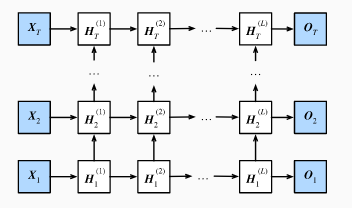
\includegraphics[width=0.6\textwidth]{deep_rnn.png}
\caption{有$L$个隐藏层的深度循环神经网络}
\end{figure}
 

具体来说, 在时间步$t$里, 设小批量输入$\mathbf{X}_t \in \mathbb{R}^{n \times d}$(样本数为$n$, 输入个数为$d$), 第$l$隐藏层($l=1, \ldots, L$)的隐藏状态为$\mathbf{H}_t^{(l)}  \in \mathbb{R}^{n \times h}$(隐藏单元个数为$h$), 输出层变量为$\mathbf{O}_t \in \mathbb{R}^{n \times q}$(输出个数为$q$), 且隐藏层的激活函数为$\phi$. 第1隐藏层的隐藏状态和之前的计算一样:
$$\mathbf{H}_t^{(1)} = \phi(\mathbf{X}_t \mathbf{W}_{xh}^{(1)} + \mathbf{H}_{t-1}^{(1)} \mathbf{W}_{hh}^{(1)}  + \mathbf{b}_h^{(1)}), $$
其中权重$\mathbf{W}_{xh}^{(1)} \in \mathbb{R}^{d \times h}$、$\mathbf{W}_{hh}^{(1)} \in \mathbb{R}^{h \times h}$和偏差 $\mathbf{b}_h^{(1)} \in \mathbb{R}^{1 \times h}$分别为第1隐藏层的模型参数. 

当$1 < l \leq L$时, 第$l$隐藏层的隐藏状态的表达式为
$$\mathbf{H}_t^{(l)} = \phi(\mathbf{H}_t^{(l-1)} \mathbf{W}_{xh}^{(l)} + \mathbf{H}_{t-1}^{(l)} \mathbf{W}_{hh}^{(l)}  + \mathbf{b}_h^{(l)}), $$
其中权重$\mathbf{W}_{xh}^{(l)} \in \mathbb{R}^{h \times h}$、$\mathbf{W}_{hh}^{(l)} \in \mathbb{R}^{h \times h}$和偏差 $\mathbf{b}_h^{(l)} \in \mathbb{R}^{1 \times h}$分别为第$l$隐藏层的模型参数. 
最终, 输出层的输出只需基于第$L$隐藏层的隐藏状态:
$$\mathbf{O}_t = \mathbf{H}_t^{(L)} \mathbf{W}_{hq} + \mathbf{b}_q, $$
其中权重$\mathbf{W}_{hq} \in \mathbb{R}^{h \times q}$和偏差$\mathbf{b}_q \in \mathbb{R}^{1 \times q}$为输出层的模型参数. 

\subsubsection{LSTM}
Long short time memory(LSTM),  由Hochreiter 和Schmidhuber提出. \citep{HochreiterLong}. 
LSTM传递两部分信息状态信息$h_{t-1}$, 记忆信息$c_{t-1}$.两者相互作用. LSTM通过门单元来动态地选择遗忘多少以前的信息和记忆多少当前的信息. 包括遗忘门, 输入门和输出门. 
$x_t$ 表示时刻t 的输入向量, $h_{t−1}$ 是时刻t−1 的循环单元的输出, 
\begin{figure}[!htb]
    \center
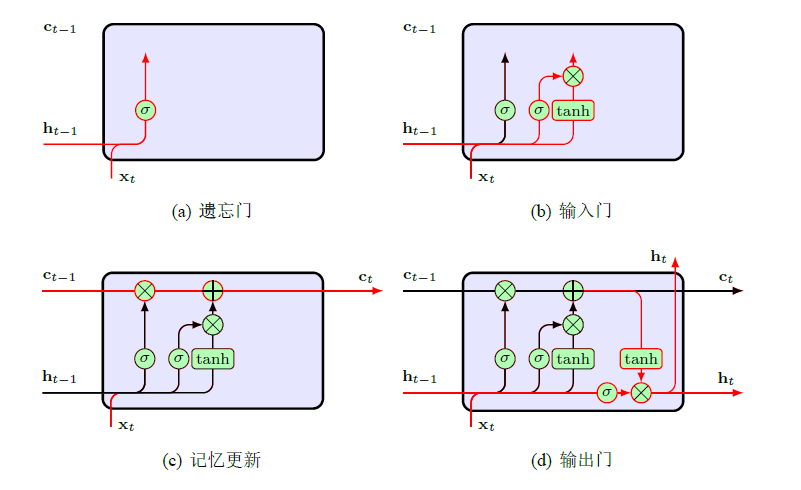
\includegraphics[width=0.9\textwidth]{LSTM.png}
\caption{LSTM 中的门控结构}
\end{figure}
LSTM结构的三部分:
\paragraph{遗忘} 通过遗忘门实现.
$f_t=\sigma (W_f h_{t-1, x_t}+b_f)$$ W_f $权值, $b_f$偏置, 该公式是对$[h_{t−1}, x_t]$ 进行变换, 并得到一个实数向量$f_t$. $f_t$ 的每一维都可以被理解为一个“门”, 它决定可以有多少信息被留下(或遗忘). 

\paragraph{记忆更新}
门控参数$\mathbf{i}_t$
\begin{align*}
    \mathbf{i}_t=\sigma(W[h_t-1, x_t])+b_i \\
    \hat{c}=Than(W_c[h_{t-1}, x_t]+b_i])
    \end{align*}

当前需记忆信息, 记为$\mathbf{i} \cdot \hat{c}_t$

\paragraph{输出}
\begin{align*}
\mathbf{o}_t  & =\sigma(W_o[h_{t-1, x_t]+b_o}) \\
\mathbf{h}_t & ={o}_t \cdot Than(c_t)
\end{align*}
 

\paragraph{循环神经网络和递归神经网络}

循环神经网络(Recurrent NN)是在时间维度上的展开, 代表信息在时间维度从前往后的的传递和积累, 可以类比markov, 后面的信息的概率建立在前面信息的基础上, 在神经网络结构上表现为后面的神经网络的隐藏层的输入是前面的神经网络的隐藏层的输出;有环结构.

递归神经网络(Recursive NN)是空间维度的展开, 是一个树结构, 无环结构.
用循环神经网络(Recurrent NN)来建模的话就是假设句子后面的词的信息和前面的词有关, 而用递归神经网络(Recursive NN)来建模的话, 就是假设句子是一个树状结构, 如由几个部分(主语, 谓语, 宾语)组成.

\subsubsection{LSTM实现}
使用周杰伦歌词, 训练模型并根据前缀“油画”创作⻓度为50个字符的⼀段歌词. 每过40个迭代周期便根据当前训练的模型创作⼀段歌词. 
\begin{figure}[!ht]
    \center
    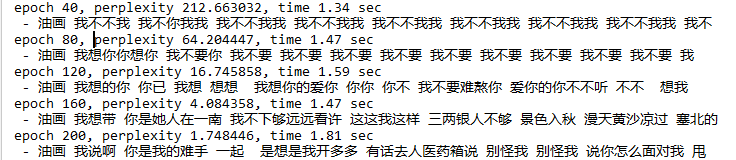
\includegraphics[width=0.8\textwidth]{lyrics.png}
    \end{figure} 
\subsubsection{GRU}
Gated Recurrent Unit (GRU) 门循环单元
\textbf{GRU 中的门控结构}

\begin{figure}[!htb]
\centering
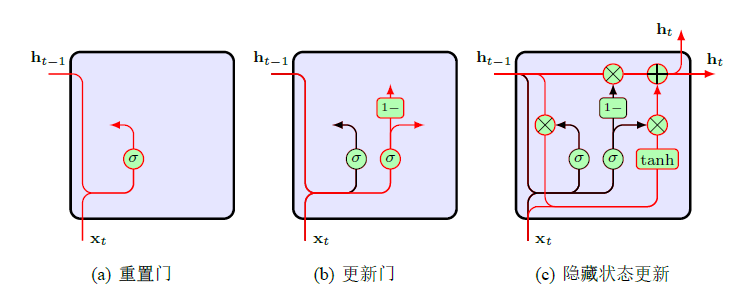
\includegraphics[width=0.9\textwidth]{GRU.png}
\caption{GRU中的门控结构}
\end{figure}

GRU对LSTM进行了简化, 把循环单元状态$h_t$和记忆$c_t$合并为状态$h_t$, 
LSTM传递的两部分信息状态信息$h_{t−1}$和记忆信息$c_{t−1}$. 
GRU有两个门, 
\begin{itemize}
    \item 重置门$r_t$:用来控制前一时刻隐藏状态的记忆程度.
    \item 更新门$u_t$:更新记忆, 使用一个门同时完成遗忘和记忆两种操作, 
\end{itemize}

GRU计算流程:

step1: 更新门$r_t$和重置门$u_t$计算
\begin{align*}
\mathbf{r}_t  & =\sigma(W_r[h_{t-1, x_t]}) \\
\mathbf{u}_t &  =\sigma(W_u[h_{t-1, x_t]})
\end{align*} 

step2: 更新当前隐藏状态 
$$\hat{h}_t=Than(W_h[r_t \cdot h_{t-1}, X_t])$$

step3: 计算更新后的隐藏状态(更新记忆)
$$h_t=(1-u_t) \cdot h_{t-1} + u_t\cdot \hat{h}_t$$

\subsubsection{改进}
\paragraph{双向模型}

\begin{figure}[htp]
    \centering
    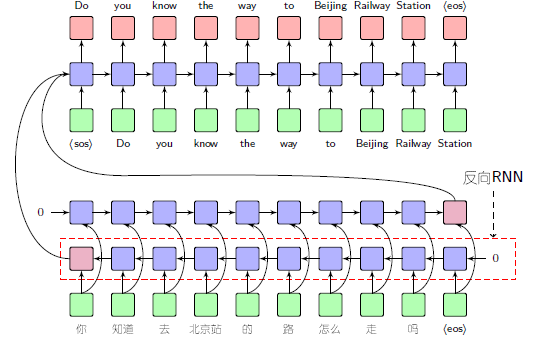
\includegraphics[width=0.9\textwidth]{dual_direction_ML.png}
    \caption{基于双向循环神经网络的机器翻译模型结构}
    \end{figure}
自左向右的模型只考虑了左侧的上下文, 因此可以用自右向左的模型对右侧上下文建模, 最终将两个模型融合同时送给编码端

\begin{figure}[htp]
    \centering
    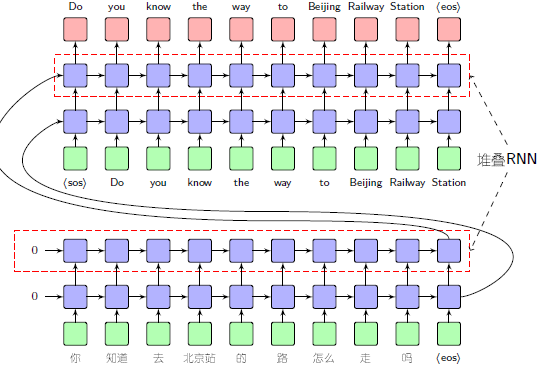
\includegraphics[width=0.9\textwidth]{multiNet_NML.png}
    \caption{基于双层循环神经网络的机器翻译模型结构}
    \end{figure}
 堆叠更多层的网络, 可以提升模型的表示能力
 
\subsection{Attention}

简单的编码器-解码器的问题:
将源语言句子编码为一个实数向量虽然很有效, 但是有明显问题
\begin{itemize}
    \item 
    整个句子编码到一个向量里可能会有信息丢失
    \item 
    缺少源语单词与目标语单词之间的对应. 某种意义上讲, 一个目标语单词的生成无法区分不同源语单词的贡献
\end{itemize}
翻译是具有很强的局部性的, 有些词之间会有更紧密的关系
源语词和目标语词的对应并不是均匀的, 甚至非常稀疏, 比如, 一些短语的生成仅依赖于源文中的少数词, 这些关系可以在表示模型中考虑
\textbf{关注的"局部性"在图像处理、语音识别等领域也有广泛讨论}
\begin{figure}[htp]
    \centering
    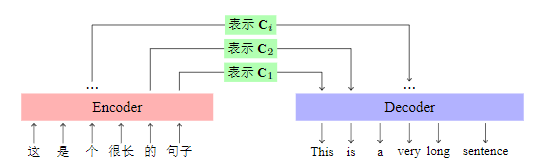
\includegraphics[width=0.9\textwidth]{attention1.png}
    \caption{使用注意力机制的翻译模型}
    \end{figure}
    \paragraph{上下文向量}
可以将注意力机制看做是一种对接收到的信息的加权处理, 上下文向量$\mathbf{C}_j$被定义为对不同时间步编码器输出的状态序列$\{ \mathbf{h}_1,  \mathbf{h}_2, ..., \mathbf{h}_m \}$进行加权求和, 如下:
    \begin{eqnarray}
    \mathbf{C}_j=\sum_{i} \alpha_{i, j} \mathbf{h}_i
    \end{eqnarray}
其中, $\alpha_{i, j}$是{\small\sffamily\bfseries{注意力权重}}\index{注意力权重}(Attention Weight)\index{Attention Weight}, 它表示目标语第$j$个位置与源语第$i$个位置之间的相关性大小. 

\begin{figure}[htp]
    \centering
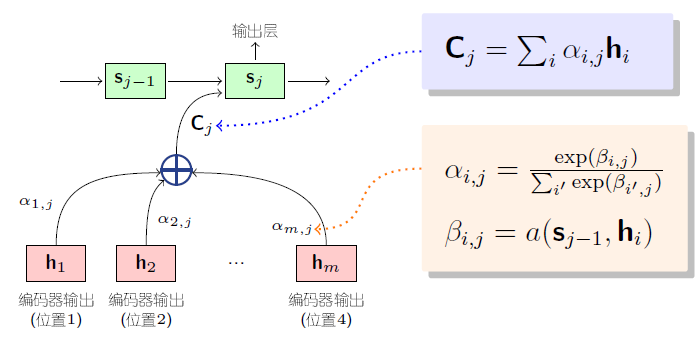
\includegraphics[width=0.9\textwidth]{context_vector_cacl.png}
    \caption{上下文向量计算过程实例}
    \end{figure}

\subsection{Transformer}
使用循环神经网络对源语、目标语建模进行信息提取效果很好, 但是当序列过长时, 词汇之间信息传递距离过长, 导致模型的信息提取能力变差. 
\begin{figure}[htp]
    \centering
    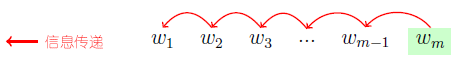
\includegraphics[width=0.9\textwidth]{self-attention1.png}
    \caption{循环神经网络中单词之间的依赖关系}
    \end{figure}
 能否将不同位置之间的词汇间信息传递的距离拉近为1? 
 \begin{figure}[htp]
    \centering
    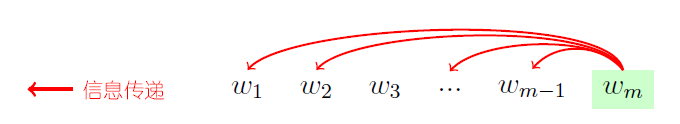
\includegraphics[width=0.9\textwidth]{self_attention2.png}
    \caption{自注意力机制中单词之间的依赖关系}
    \end{figure}


\textbf{自注意力机制(Self-Attention)}可以很好的解决长距离依赖问题, 增强信息抽取能力, 在长距离语言建模任务取得了很好的效果
 自注意力机制则是将源语言每个位置的表示$h_i$看做query, 同时将所有位置的表示看做key和value
 Transformer是Google在2017年提出的一个新型网络结构, 完全基于注意力机制, 取得了很好成绩!通过自注意机制能够直接获取全局信息, 不像RNN需要逐步进行信息提取, 也不像CNN只能获取局部信息, 可以并行化操作, 提高训练效率, Transformer不仅仅被用于神经机器翻译任务, 还广泛用于其他NLP任务、甚至图像处理任务. 
 %----------------------------------------------
\begin{figure}[ht]
    \centering
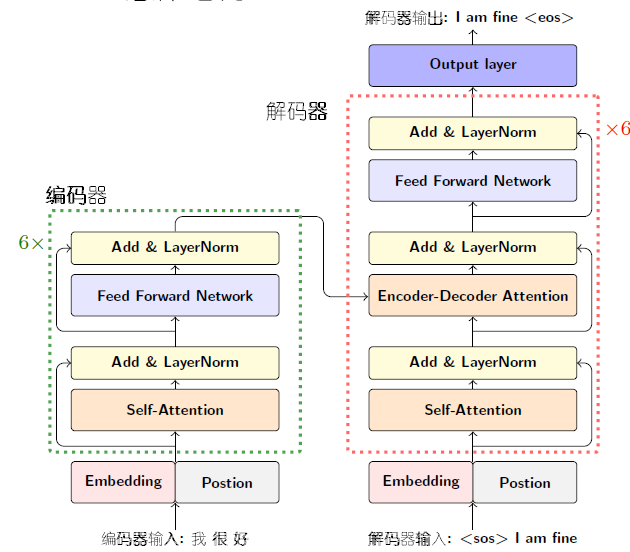
\includegraphics[width=0.9\textwidth]{Transformer1.png}
    \caption{Transformer结构}
    \label{Transformer}
    \end{figure}
    \parinterval 图\ref{Transformer} 展示了经典的Transformer结构. 解码器由若干层组成(绿色虚线框就代表一层). 每一层(layer)的输入都是一个向量序列, 输出是同样大小的向量序列, 而Transformer层的作用是对输入进行进一步的抽象, 得到新的表示结果. 不过这里的层并不是指单一的神经网络结构, 它里面由若干不同的模块组成, 包括:
    \begin{itemize}
        \vspace{0.5em}
        \item {\small\sffamily\bfseries{自注意力子层}}\index{自注意力子层}(Self-attention Sub-layer)\index{Self-attention Sub-layer}:使用自注意力机制对输入的序列进行新的表示;
        \vspace{0.5em}
        \item {\small\sffamily\bfseries{前馈神经网络子层}}\index{前馈神经网络子层}(Feed-forward Sub-layer)\index{Feed-forward Sub-layer}:使用全连接的前馈神经网络对输入向量序列进行进一步变换;
        \vspace{0.5em}
        \item {\small\sffamily\bfseries{残差连接}}\index{残差连接}(Residual Connection, 标记为``Add'')\index{Residual Connection}:对于自注意力子层和前馈神经网络子层, 都有一个从输入直接到输出的额外连接, 也就是一个跨子层的直连. 残差连接可以使深层网络的信息传递更为有效;
        \vspace{0.5em}
        \item {\small\sffamily\bfseries{层正则化}}\index{层正则化}(Layer Normalization)\index{Layer Normalization}:自注意力子层和前馈神经网络子层进行最终输出之前, 会对输出的向量进行层正则化, 规范结果向量取值范围, 这样易于后面进一步的处理. 
        \vspace{0.5em}
        \end{itemize}

\subsubsection{残差连接}
在Transformer中, 编码器、解码器分别由6层网络组成, 每层网络又包含多个子层(自注意力网络、前馈神经网络). Transformer实际上是一个很深的网络结构, 在训练过程中容易出现梯度消失的情况在这里引入了在图像领域用来训练深层网络的技术, 残差网络来避免上述问题.
\begin{eqnarray}
    x_{l+1} = x_l + \mathcal{F} (x_l)
    \end{eqnarray}

    在Transformer的训练过程中, 由于引入了残差操作, 将前面所有层的输出加到一起. 这样会导致高层的参数分布不断变大, 造成训练过程不稳定、训练时间较长. 为了避免这种情况, 在每层中加入了层正则化操作I 使用均值和方差对样本进行平移缩放, 将数据规范化为均值为0, 方差为1的标准分布
    \begin{eqnarray}
        \textrm{LN}(x) = g \cdot \frac{x- \mu} {\sigma} + b
        \end{eqnarray}  


\subsubsection{机器翻译系统简介}


基于规则、基于统计、基于实例、神经网络方法
不同机器翻译方法有不同的特点.  
\begin{enumerate}
    \item 规则系统需要人工书写规则并维护, 人工代价较高. 统计和神经网络方法仅需要设计特征或者神经网络结构, 对人工依赖较少(语言相关的). 
    \item 基于实例、统计和神经网络的方法都需要依赖语料库(数据), 其中统计和神经网络方法具有一定的抗噪能力, 因此也更适合大规模数据情况下的机器翻译系统研发. 
    \item  基于规则和基于实例的方法在受限场景下有较好的精度, 但是在开放领域的翻译上统计和神经网络方法更具优势. 
\end{enumerate}

\begin{table}  [!htb]
    \Large  
    \caption{不同机器翻译方法的对比}  
    \begin{center}  
    \begin{tabular}{l|lll l}  
    \hline  
    &规则&实例&统计&神经 \\ \hline
    人工写规则&是&否&否&否\\ 
    人工代价&高&一般&几乎没有&几乎没有\\ 
    数据驱动&否&是&是&是\\ 
    依赖数据质量&N/A&高&低&较低\\ 
    抗噪声能力&低&低&高&较高\\ 
    使用范围&受限领域&受限领域&通用领域&通用领域\\ 
    翻译精度&高&较高&不确定&不确定\\  
    \hline  
    \end{tabular}  
    \end{center}  
    \end{table}

\subsection{基于梯度的方法的改进}
 \subsubsection{动量法Momentum}
 对于普通的梯度下降法 $\theta \leftarrow \theta - \eta \nabla f(x)$,  当接近最优值时梯度会比较小, 由于学习率固定, 普通的梯度下降法的收敛速度会变慢, 有时甚至陷入局部最优.   
设时间步$t$的自变量为${x}_t$, 学习率为$\eta_t$. 
在时间步$0$, 动量法创建速度变量$\mathbf{v}_0$, 并将其元素初始化成0. 在时间步$t>0$, 动量法对每次迭代的步骤做如下修改:
 $$
 \begin{aligned}
 \mathbf{v}_t &\leftarrow \gamma \mathbf{v}_{t-1} + \eta_t \mathbf{g}_t,  \\
 \mathbf{x}_t &\leftarrow \mathbf{x}_{t-1} - \mathbf{v}_t, 
 \end{aligned}
 $$
 其中$\mathbf{g}_t$同小批量随机梯度中的定义.

 \paragraph{指数加权移动平均exponentially weighted moving average}
 给定超参数$0 \leq \gamma < 1$, 当前时间步$t$的变量$y_t$是上一时间步$t-1$的变量$y_{t-1}$和当前时间步另一变量$x_t$的线性组合:
 $$y_t = \gamma y_{t-1} + (1-\gamma) x_t.$$

对$y_t$展开:

 $$
 \begin{aligned}
 y_t  &= (1-\gamma) x_t + \gamma y_{t-1}\\
          &= (1-\gamma)x_t + (1-\gamma) \cdot \gamma x_{t-1} + \gamma^2y_{t-2}\\
          &= (1-\gamma)x_t + (1-\gamma) \cdot \gamma x_{t-1} + (1-\gamma) \cdot \gamma^2x_{t-2} + \gamma^3y_{t-3}\\
          &\ldots
 \end{aligned}
 $$
 
 令$n = 1/(1-\gamma)$, 那么 $\left(1-1/n\right)^n = \gamma^{1/(1-\gamma)}$. 
 
 $$ \lim_{n \rightarrow \infty}  \left(1-\frac{1}{n}\right)^n = \exp(-1) \approx 0.3679, $$
 当$\gamma \rightarrow 1$时, $\gamma^{1/(1-\gamma)}=\exp(-1)$, 如$0.95^{20} \approx \exp(-1)$. 如果把$\exp(-1)$当作一个比较小的数, 我们可以在近似中忽略所有含$\gamma^{1/(1-\gamma)}$以及更高阶的系数的项.  
 $y_t$可看作是对最近$1/(1-\gamma)$个时间步的$x_t$值的加权平均. 


对动量法的速度变量做变形:

 $$\mathbf{v}_t \leftarrow \gamma \mathbf{v}_{t-1} + (1 - \gamma) \left(\frac{\eta_t}{1 - \gamma} \mathbf{g}_t\right). $$
$\mathbf{v}_t$实际上对序列$\{\eta_{t-i}\mathbf{g}_{t-i} /(1-\gamma):i=0, \ldots, 1/(1-\gamma)-1\}$做了指数加权移动平均. 在动量法中, 自变量在各个方向上的移动幅度同时取决于当前梯度和过去的各个梯度在各个方向上是否一致. 

若用 $G_t$表示第t轮迭代的动量,  $g_t$表示第t轮迭代的更新量, 当 $t \to \infty $,  $G_t= \frac{g_0}{1-\gamma} $, 如果梯度保持不变, 最终的更新速度会是梯度项乘以学习率的 $\frac{1}{1-r}$ 倍. 

\subsubsection{AdaGrad}
\paragraph{问题} 假设目标函数为$f$, 自变量为一个二维向量$[x_1,  x_2]^\top$, $x_1, x_2$在迭代时都使用相同的学习率. 若两者梯度值差别较大, 选择一个小学习率会使在梯度值较小的维度迭代过慢. 
\paragraph{解决方法}: 不同维度设置不同学习率. 

AdaGrad算法使用一个小批量随机梯度$\mathbf{g}_t$按元素平方的累加变量$\mathbf{s}_t$.  $\mathbf{s}_0$中每个元素初始化为0. 在$t$时刻, 累积平方梯度:
$$\mathbf{s}_t \leftarrow \mathbf{s}_{t-1} + \mathbf{g}_t \odot \mathbf{g}_t, $$
其中$\odot$是按元素相乘. 
之后, 将自变量中每个元素的学习率通过按元素运算重新调整:
$$\mathbf{x}_t \leftarrow \mathbf{x}_{t-1} - \frac{\eta}{\sqrt{\mathbf{s}_t + \epsilon}} \odot \mathbf{g}_t, $$
其中$\epsilon$是为了维持数值稳定性而添加的常数.  

\subsubsection{RMSProp}
\textbf{问题}: 因为调整学习率时分⺟上的变量$s_t$⼀直在累加按元素平方的小批量随机梯度, 所以⽬标函数⾃变量每个元素的学习率在迭代过程中⼀直在降低(或不变). 因此, 当学习率在迭代早期降得较快且当前解依然不佳时, AdaGrad算法在迭代后期由于学习率过小, 可能较难找到一个有用的解. 

 \textbf{解决方法:} 改变Adagrad梯度积累为指数加权的移动平均. 
 
给定超参数$0 \leq \gamma < 1$, RMSProp算法在时间步$t>0$计算

$$\mathbf{s}_t \leftarrow \gamma \mathbf{s}_{t-1} + (1 - \gamma) \mathbf{g}_t \odot \mathbf{g}_t. $$

将目标函数自变量中每个元素的学习率通过按元素运算重新调整, 然后更新自变量

$$\mathbf{x}_t \leftarrow \mathbf{x}_{t-1} - \frac{\eta}{\sqrt{\mathbf{s}_t + \epsilon}} \odot \mathbf{g}_t,  $$

其中$\epsilon$是为了维持数值稳定性而添加的常数. 自变量每个元素的学习率在迭代过程中就不再一直降低(或不变). 
\subsubsection{AdaDelta}
\paragraph{问题:}同RMSProp待解决问题相同 \\
\textbf{解决方法:}不设置学习率, 用一阶的方法, 近似模拟二阶牛顿法. 使用了小批量随机梯度$\mathbf{g}_t$按元素平方的指数加权移动平均变量$\mathbf{s}_t$. 

在时间步0, 它的所有元素被初始化为0. 给定超参数$0 \leq \rho < 1$], 

在时间步$t>0$
$$\mathbf{s}_t \leftarrow \rho \mathbf{s}_{t-1} + (1 - \rho) \mathbf{g}_t \odot \mathbf{g}_t. $$

状态变量$\Delta\mathbf{x}_t$, 在时间步0时被初始化为0. $\Delta\mathbf{x}_{t-1}$是来计算自变量的变化量:

$$ \mathbf{g}_t' \leftarrow \sqrt{\frac{\Delta\mathbf{x}_{t-1} + \epsilon}{\mathbf{s}_t + \epsilon}}   \odot \mathbf{g}_t,  $$

其中$\epsilon$是为了维持数值稳定性而添加的常数, 如$10^{-5}$. 

更新自变量:
$$\mathbf{x}_t \leftarrow \mathbf{x}_{t-1} - \mathbf{g}'_t. $$

最后, $\mathbf{g}'_t$按元素平方的指数加权移动平均:
$$\Delta\mathbf{x}_t \leftarrow \rho \Delta\mathbf{x}_{t-1} + (1 - \rho) \mathbf{g}'_t \odot \mathbf{g}'_t. $$

可以看到, 如不考虑$\epsilon$的影响, AdaDelta算法与RMSProp算法的不同之处在于使用$\sqrt{\Delta\mathbf{x}_{t-1}}$来替代超参数$\eta$. 

\subsubsection{Adam} \citep{Kingma2014Adam}
Adam可以理解为加了Momentum 的 RMSprop, 然后修正偏差.
\begin{figure}[htp]
    \centering
     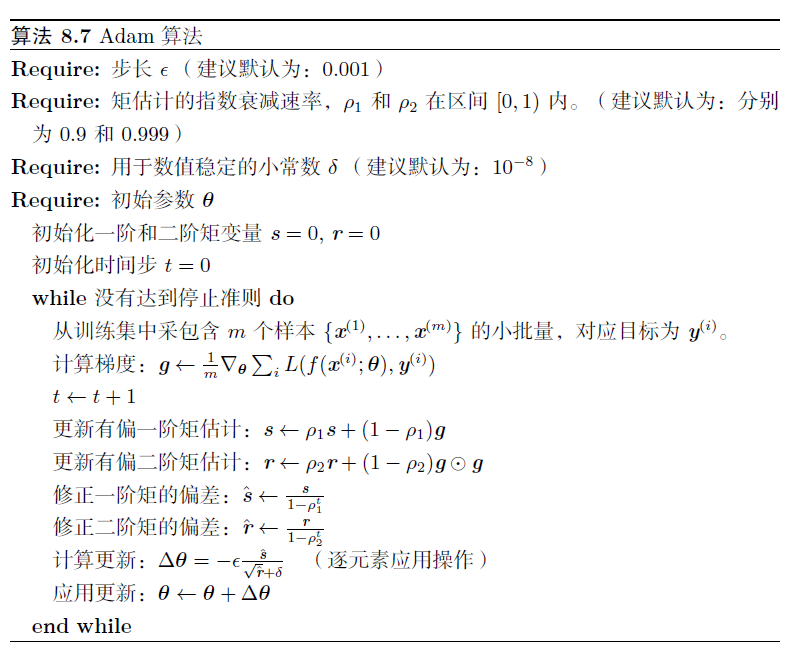
\includegraphics[width=0.8\textwidth]{adam.png}
 
    \label{fig:adm}
    \end{figure}

\subsection{建模}

\parinterval 在给定源语言句子$\mathbf{x}$的情况下, 找出翻译概率最大的目标语译文$\hat{\mathbf{y}}$:
\begin{eqnarray}
\hat{\mathbf{y}} = \argmax_{\mathbf{y}} \textrm{P} (\mathbf{y} | \mathbf{x})
\end{eqnarray}

\noindent 这里, 用$\mathbf{x}=\{ x_1, x_2, ...,  x_m \}$表示输入的源语言单词序列, $\mathbf{y}=\{ y_1, y_2, ...,  y_n \}$ 表示生成的目标语单词序列. 由于神经机器自左向右逐词翻译, 并且考虑之前的结果, 因此对$\textrm{P} (\mathbf{y} | \mathbf{x})$的求解可以转换为:
\begin{eqnarray}
\textrm{P} (\mathbf{y} | \mathbf{x}) = \prod_{j=1}^{n} \textrm{P} ( y_j | \mathbf{y}_{<j },  \mathbf{x}  )
\end{eqnarray}
$ \mathbf{y}_{<j }$表示目标语第$j$个位置之前已经生成的译文单词序列. 

\parinterval 求解$\textrm{P}(y_j | \mathbf{y}_{<j}, \mathbf{x})$有三个关键问题(图\ref{fig:probquestion}):

\begin{itemize}
\item	{\small\sffamily\bfseries{词嵌入}}(Word Embedding):$\mathbf{x}$和$\mathbf{y}_{<j }$的分布式表示. 将源语言单词转化为实数向量. 可以把这个过程记为$\textrm{e}_x (\cdot)$. 类似的, $\mathbf{y}_{<j }$记为$\textrm{e}_y (\cdot)$. 
\item	在词嵌入的基础上获取整个序列的表示, 即句子的{\small\sffamily\bfseries{表示学习}}(Representation Learning). 如图\ref{fig:probquestion}中, 编码器最后一个循环单元的输出$\mathbf{h}_m$被看作是一种包含了源语句子信息的表示结果, 记为$\mathbf{C}$. 
\item	得到每个目标语单词的概率, 即译文单词的{\small\sffamily\bfseries{生成}}Generation). 可以用一个Softmax输出层来获取当前时刻所有单词的分布.令目标语序列$j$时刻的循环神经网络的输出向量(或状态)为$\mathbf{s}_j$. $ y_j$的生成只依赖前一个状态$\mathbf{s}_{j-1}$和当前时刻的输入. 同时考虑源语言信息$\mathbf{C}$, $\textrm{P}(y_j  | \mathbf{y}_{<j}, \mathbf{x})$可以被重新定义为:
\begin{eqnarray}
\textrm{P} (y_j | \mathbf{y}_{<j}, \mathbf{x}) \equiv \textrm{P} ( {y_j | \mathbf{s}_{j-1} , y_{j-1}, \mathbf{C}} )
\end{eqnarray}
可以进一步简化为, 
\begin{eqnarray}
\textrm{P} (y_j | \mathbf{y}_{<j}, \mathbf{x}) \equiv
 \left \{ \begin{array}{ll}
\textrm{P} (y_j |\mathbf{C} , y_{j-1}) &j=1 \\
\textrm{P} (y_j|\mathbf{s}_{j-1}, y_{j-1})  \quad &j>1
\end{array} \right . 
\end{eqnarray}
\end{itemize}

\begin{figure}[htp]
    \centering
     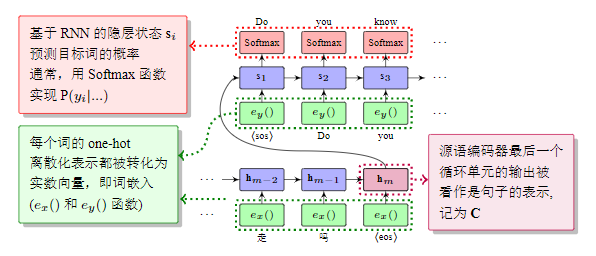
\includegraphics[width=0.8\textwidth]{RNNprobquestion.png}
    \caption{求解$\textrm{P} (y_j | \mathbf{y}_{<j}, \mathbf{x})$的三个基本问题}
    \label{fig:probquestion}
    \end{figure}

\begin{figure}[htp]
\centering
    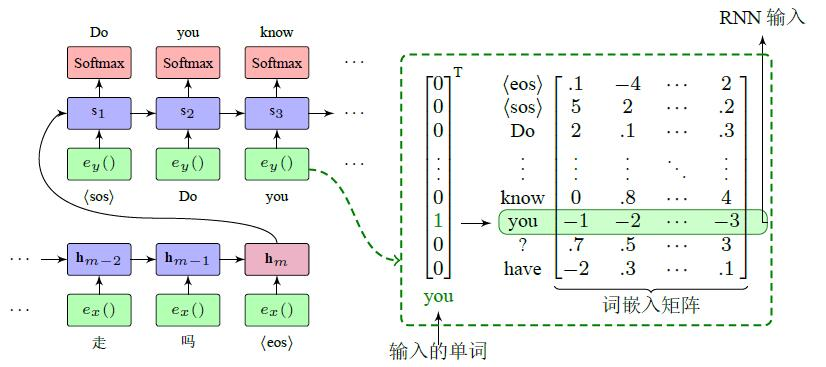
\includegraphics[width=0.8\textwidth]{figures/MachineTranslation/fig6-12.jpg}
\caption{词嵌入的生成过程}
\label{fig:genWordEmbedded}
\end{figure}

    \parinterval 如何在神经机器翻译系统中获得单词的词嵌入表示?这里引入一个词嵌入层对输入的单词进行词嵌入表示, 即图\ref{fig:genWordEmbedded}中的绿色方框部分. 假设输入的单词$y_j$已经被表示为One-hot形式(行向量). 词嵌入层的工作就是把One-hot向量右乘一个实数矩阵$\mathbf{E}$, 得到的结果(行向量)就是这个单词所对应的词嵌入结果. 
    \begin{eqnarray}
    \textrm{e}_y (y_j) = y_j \mathbf{E} 
    \end{eqnarray} 

    \noindent 这里, $\mathbf{E}$也被称作词嵌入矩阵, 它可以作为模型的一部分参数共同参与机器翻译系统的训练, 也可以由外部其他模块训练得到(如预训练模型). $\mathbf{E}$的大小为$|V| \times d$, 这里$|V|$表示词表$V$的大小, $d$表示循环神经网络输入和输出向量的维度. 
    

    词嵌入的作用是把离散化的单词表示转换为连续空间上的分布式表示
    \begin{enumerate}
        \item   把输入的词转换成唯一对应的词表大小的0-1向量
        \item 根据0-1向量, 从词嵌入矩阵中取出对应的词嵌入$e(\cdot)$
        \item 取出的词嵌入$e(\cdot)$作为循环神经网络的输入
    \end{enumerate} 
  
    
    
\begin{figure}[htp]
    \centering
    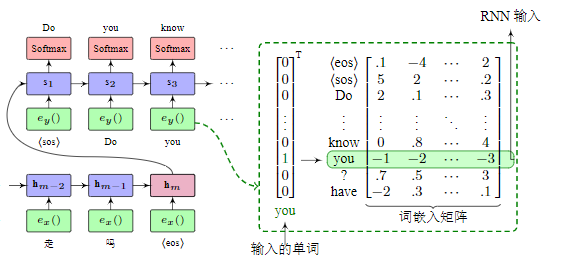
\includegraphics[width=0.8\textwidth]{NMLEmbed.png}
    \caption{词嵌入的生成过程}
 
    \end{figure}

输出层需要得到每个目标语单词的生成概率, 进而选取概率最高的词作为输出. 但RNN中的隐藏层并不会输出单词概率, 而是输出s, 其每一行对应一个单词表示.
s经过权重矩阵W变成$\hat{s}$, 其隐藏层维度变换成词表的大小
$\hat{s}$经过Softmax变换得到不同词作为输出的概率, 即单词i的概率
$$p_i= Softmax(i) = \frac{{e^{\hat{s}_i}}}{{\sum_j e^{\hat{s}_j}}}$$
 


    \begin{figure}[htp]
        \centering
        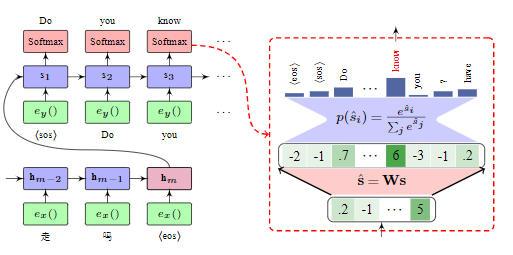
\includegraphics[width=0.8\textwidth]{outputpredict.png}
        \caption{输出层的预测过程} 
        \end{figure}

\subsubsection{RNN训练}
训练RNN我们通常会使用Adam或者SGD两种优化器, 它们各有优劣. Adam 通用, 性能不是最好, SGD  一个任务一个配置, 效果更好. 
因此需要快速得到模型看一下初步效果, 选择Adam. 
若是需要在一个任务上得到最优的结果, 选择SGD. 
需要注意的是, 训练RNN的时候, 我们通常会遇到梯度爆炸的问题, 也就是梯度突然变得很大, 这种情况下需要使用梯度裁剪来防止梯度超过阈值. 

% \section{Private Empirical Risk Minimization}
 
如图\ref{fig:privacy_data_accuracy}, 在考虑个人隐私的情况下,数据集大小,隐私水平和精确度是机器学习模型训练需考虑的三个变量, 三个量互相关.
一般情况下,我们可以考虑得到图中两个角的较好值, 算法根据三个变量的取舍而又有所不同. (数据量大还是)

线性分类模型的隐私泄露问题。直观地,在一维情况下,线性分类器会返回样本的中位数,而中位数通常是一个具体样本的取值,那么这个样本的即被暴露给了获得模型的使用者,我们认为这侵犯到了他的隐私。在高维情况下依然存在相似的情况。\cite{kasiviswanathan2012power}

从隐私保护的角度讲,从原始输入到输出找到一处进行截断,在其中加入一道隐私保护屏障,具体在哪一步截断则对应于不同的方法。
\begin{figure}
    \centering
    \label{fig:privacy_data_accuracy}
    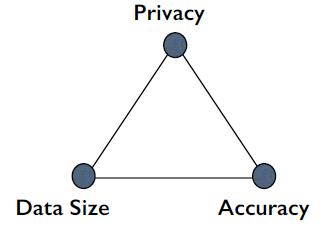
\includegraphics[width=0.3\textwidth]{figures/priacy_data_accuracy.jpg}
    \caption{the relationship of data size, priacy and accuracy}
\end{figure}
\begin{itemize}
    \item \emph{输入扰动 Input perturbation} 输入扰动在获取数据时直接为数据添加上噪声,之后的计算基于添加了噪声的数据。优点:易于实现,可重复使用经过消毒的数据集。\cite{DJW13,KTS17}
    \item \emph{目标扰动 Objective Perturbation} 目标扰动在目标函数中添加一个随机量,以导出最终模型输出的随机性,对目标做随机逼近:随机性取决于J(w)的敏感性属性。 \cite{CMS11,ZZXYW12}
    \item \emph{优化扰动 optimization Perturbation} 优化扰动在执行最小化的过程中,设计满足于差分隐私的优化算法
    \item \emph{输出扰动 Output Perturbation } 输出扰动是最简单直接的Laplace Mechanism思路延续下来的方法,基于输出(模型参数)的敏感度对模型添加噪声,不需要重新设计的基线算法. \cite{CMS11,RBHT12}
\end{itemize}
 
\begin{figure}
    \centering
    \label{fig:estimation_prediction}
    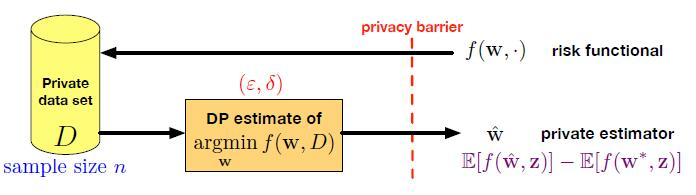
\includegraphics[width=0.7\textwidth]{figures/estimation_prediction.jpg}
    \caption{Statistical estimation}
\end{figure}

统计估计:根据未来数据的良好预期性能,估计一个参数或预测指标。
目标:良好的隐私样本大小权衡
隐私 差分隐私对数据分配没有任何假设:隐私是无条件的。
准确度-准确度度量, 也即“真正的人口分配”:预期的过度统计风险。


$w^* =\min_w \frac{1}{n} \Sigma_{i=1}^n \ell(w,(x_i,y_i)) + \lambda R(w)$
其中  $\lambda R(w)$为抑制过拟合的正则项.


\paragraph{差分隐私优化算法}

\begin{itemize}
\item大数据集是优化的挑战:批(batch)方法不可行
\item使用更多的数据可以帮助我们更好权衡:更好的隐私和准确性
\item在线学习涉及多个版本:可能会有更多的隐私损失
\end{itemize}


目标:使用优化算法保证隐私
机器学习中常见的经验损失最小化方法

$$w^* =\min_w \frac{1}{n} \Sigma_{i=1}^n \ell(w,(x_i,y_i)) + \lambda R(w)$$
中  $\lambda R(w)$为抑制过拟合的正则项.


Non-private SGD 非隐私差分梯度下降

$J(w)=\frac{1}{n} \Sigma_{i=1}^n \ell(w,(x_i,y_i)) + \lambda R(w)$
加噪的隐私随机梯度下降

 


\paragraph{ 实践中遇到的问题}

\begin{itemize}
    \item  Theoretical analysis is for fixed privacy parameters –how should we choose them in practice?
    \item Given a data set, can I tell what the privacy-utilitysample-size tradeoff is?
\item What about more general optimization problems/algorithms?
\item What about scaling (computationally) to large data sets?
\end{itemize}
% 
\section{CPFed: Communication-Efficient and Privacy-Preserving Federated Learning}

\subsection{摘要}
\paragraph{挑战:} 在联邦学习的迭代过程中, 边缘设备需要计算结果后上传到服务器进行更新. 在这个过程中, 会导致隐私泄露和\textbf{通信开销}上升. 
\paragraph{应对:} 本文提出\textbf{CPFed}, 一种通信高效和保护隐私的联邦学习方法.
\paragraph{CPFed组件:} 
\begin{enumerate}[label=(\arabic*)]  
    \item 周期性平均, 即仅在服务器上周期性平均边缘设备的本地计算结果;
    \item 高斯机制, 边缘器件在将计算结果发送到服务器之前随机扰动其本地计算结果;
    \item 安全聚合, 其中扰动的本地计算结果在发送到服务器之前同态加密. 
\end{enumerate}
\paragraph{本文工作:} 给出了CPFed的\textbf{端到端隐私保证}, 并分析了其在凸模型和非凸模型上的理论收敛速度. 通过在真实数据集上的大量数值实验, 证明了方法的有效性和效率. 
\paragraph{结果:}CPFed可以解决联邦学习中的通信效率和隐私泄露问题, 同时获得较高的模型精度.  \cite{hu2020cpfed}

\paragraph{贡献}
\begin{enumerate}
    \item 提出CPFed新型联邦学习方案CPFed, 在没有完全可信的服务器的情况下, 通过分布式数据进行高效的、差异化的私有学习. 
    \item CPFed通过允许部分设备在每次迭代时参加培训并定期与服务器通信来减少通信数量. 
    \item 在不降低模型精度的情况下, CPFed通过集成安全聚合和不同隐私技术, 严格保护每个设备的数据隐私. 
    \item 零集中的差异隐私密切考虑CPFed的端到端隐私损失. 
    \item  对强凸和非凸损失函数进行CPFed的收敛分析, 并基于真实数据集进行广泛的评估. 
\end{enumerate}

\subsection{背景介绍}

\subsubsection{挑战}

\paragraph{通信开销}
虽然联邦学习中边缘设备和服务器只传递模型更新, 但是可能包含(深度神经网络的)数亿个参数, 而且需要多次迭代才能获得较高精度模型. 边缘设备大多资源受限(带宽有限,特别是上行传输时).
\paragraph{隐私泄露}
只传输模型更新不足以保证隐私安全. 例如难以抵御重构攻击和成员推理攻击.


\subsubsection{差分隐私DP}
\paragraph{$(\varepsilon,\delta)-DP$} 
随机算法$\mathcal{M:D \to R}$, 其中定义域$\mathcal{D}$, 值域$\mathcal{R}$
\begin{equation}
    Pr [ \mathcal{M}(D) \in S ] \leqslant \exp(\epsilon c) \cdot Pr [ \mathcal{A(D_2)} ] \in S  + \delta 
\end{equation}

其中,$D, D^{'} \in \mathcal{D}$为两个两个数据集, 输出 $S \in \mathcal{O}$, $\varepsilon$称为预定隐私.
可以在输出加上高斯噪声.

\paragraph{$\rho$零集中DP($\rho-\text{zCDP}$)}
$\rho-\textbf{zCDP}$具有紧密的组合约束, 更适合分析迭代算法的端到端隐私损失. 
$\rho-\textbf{zCDP}$满足
\begin{equation}
    \mathbb{E}[e^{(\alpha-1)Z}] \leqslant e^{(\alpha -1)\rho}
\end{equation} 
其中\subparagraph{隐私损失} 
\begin{equation}
    Z := \log \frac{Pr[\mathcal{M}(D)]=o}{Pr[\mathcal{M}(D^{'})]=o} 
\end{equation}

其中$o \in \mathcal{R}$
$\rho-\textbf{zCDP}$的性质

\begin{figure}[ht]
    \setlength{\abovecaptionskip}{0.1cm}
    \centering    
    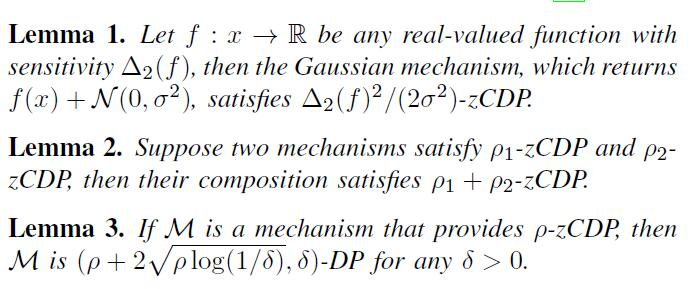
\includegraphics[width=0.7\textwidth]{CPFed/zCDPLemma.jpg}
    \caption{$\rho-\textbf{zCDP}$性质}
\end{figure}

\subsection{系统建模}
\subsubsection{联邦学习系统}
联邦学习吸引包含n个客户机, 每个有$m$条数据, 表示为$D_i = {\xi^i_1, \ddot,\xi^i_m}$
\textbf{客户机目标}是训练一个共同模型 $\theta \in \mathbb{R}^d$, 即最小化所有本地数据的联合最小经验损失.
\begin{equation}
    \min_\theta f(\theta) := \frac{1}{n} \sum^n_{i=1}f_i(\theta) \ \  \text{其中},f_i(x) := \frac{1}{m}\sum_{\xi\in D_i} l(\theta , \xi ) 
\end{equation}
其中$f_i$是客户机$i$的局部目标函数,$l(\theta; \xi)$是模型$\theta $在点$\xi\in D_i $处的损失.

\subsubsection{威胁}
本文假设对手有两类:
\begin{enumerate}
    \item “诚实但好奇”的中央服务器或客户机. 中央服务器将忠实地遵循设计的培训协议, 但会对客户机的私有数据感到好奇, 并可能从共享的消息中推断真实信息. 
    \item 被动的攻击者:在训练中窃听共享消息,但不主动攻击.
\end{enumerate}


\subsubsection{目标}
设计一个方案使客户机以低成本通信成本训练模型并保证隐私.

\subsection{CPFed}

\subsubsection{提高通信效率--周期平均}
\paragraph{问题} 起初方法--分布式SGD,由于通信速度比本地慢数个数量级,且联邦学习通常设备过多,导致总体效率低下.

\paragraph{改进方法}
同时减少通信轮的数量和每轮涉及的客户端, 如图2所示. 在我们的方法中, 服务器首先均匀随机地选择一组客户端, 然后让选中的客户端执行多次迭代以最小化本地目标, 然后再将其本地计算结果发送给服务器. 
简单来说,就是分组分级策略,相当于联邦的每个州继续往下分为各县. 各县先统计好本地数据再提交. 这和小批量随机梯度下降的思想相似.
在第$t$轮迭代是,一组$r$个客户机$\Omega_t$通过$\tau$次局部训练预先训练模型$\theta^t$,
用$\theta_i^{t,s}$表示第$t$轮迭代的第$s$轮局部迭代的客户机$i$的局部模型.

\begin{equation}
    \theta^{t,s+1}_i= \theta_i^{t,s}- \eta g(\theta_i^{t,s})
\end{equation}
其中 $g(\theta_i^{t,s}) := \frac{1}{B} \sum_{X_i} \nabla l(\theta_i^{t,s,\xi)}$表示基于一批B条数据$X_i$的小批量随机梯度下降计算. 

$\tau$轮迭代后,服务器共享模型更新为 
\begin{equation}
    \theta^{t+1}=\frac{1}{r} \sum_{i\in \Omega_t} \theta_i^{t,\tau} 
\end{equation}
 

\begin{figure}[ht]
    \
    \setlength{\abovecaptionskip}{0.1cm}
    \centering    
    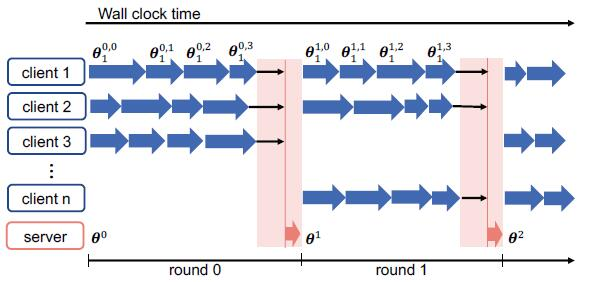
\includegraphics[width=0.7\textwidth]{CPFed/communication-reduction.jpg}
    \label{communication-reduction-strategies}
    \caption{$\tau=4,r=3 $时的通信减少策略}
\end{figure}
 
\subsubsection{防止隐私泄露--DP}

\paragraph{问题} 通信减少策略不能阻止更高级的攻击(推断)
\paragraph{设计目标} $\theta_t$和${\theta_i^{t, \tau}}_{i\in\Omega_t}$包含隐私数据,通过DP防止两种隐私泄露
\paragraph{设计}

\begin{equation}
    \theta_i^{t,s+1}= \theta_i^{t,s}- \eta (g(\theta_i^{t,s})) + b_i{t,s} 
    \label{local_iter}
\end{equation}
其中 $b_i{t,s}$是第$t$轮迭代的第$s$次局部迭代时取样自分布$N(0,\sigma^2 \mathbf{1}_d)$的高斯噪声

\paragraph{结果} 由于DP的后处理特性, 局部模型的和$\theta^{t+1}$ 为客户端保留和本地模型{\color{red}相同级别的DP保证 }

\subsubsection{提升模型精确度--安全集聚}

\paragraph{问题} 由于使用高斯机制的差分隐私,模型精确度将会下降
\paragraph{分析} 服务器只需知道本地模型的平均值,可以隐藏单个本地模型,减少客户端隐私损失
\paragraph{设计目标} 设计基于秘密共享的协议,安全聚合应能够达到以下目标
\begin{enumerate}[label=(\arabic*)]  
    \item 隐藏客户端的单个消息
    \item 恢复每一轮随机客户端的单个消息总和, 
    \item 使参与的客户端的通信成本较低. 
\end{enumerate}


\paragraph{设计}
提出的安全协议包括以下两个步骤:
\begin{enumerate}[label=(\arabic*)]  
    \item 加密上传:$\Omega_t$中的客户机上传自己的加密本地模型$\{ c_i^t\} I{i\in \Omega_t}$到服务器
\item 解密:服务器解密来自客户机组$\Omega_t$的消息和. 

\end{enumerate}

 
安全协议的基本思想是在明文中添加随机数$r_i^t$来保护客户机$i$的信息$p_i^t$.即$c^t_i = p^t_i +r^t_i$,难点在于使所有客户机的$r^t_i$和为0, 消除随机数的影响. 但是这要求客户机相互通信,这会导致低效通信.

解决方案是引入伪随机函数(PRF)$G$

PRF $G$要求在初始化和第$t$轮迭代时客户机$i$和$j$统一随机数种子$seed_{i,j}$,,并且每轮循环输出不同的伪随机数$G(seed_{i,j},t)$. 这样每次客户机无需经过和其他客户机交互便可计算出$r_i^t$, 便可降低通信开销.

\begin{figure}[ht]
    \
    \setlength{\abovecaptionskip}{0.1cm}
    \centering    
    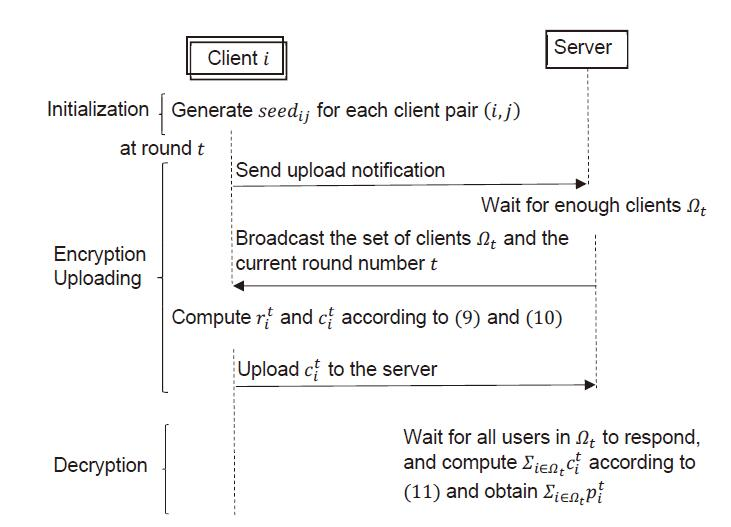
\includegraphics[width=0.7\textwidth]{CPFed/secure-aggregation.jpg}
    \caption{CPFed中的高效安全聚合协议}
\end{figure}
 
\paragraph{加密过程}
在客户机组$\Omega$中,客户机$i \in \Omega_t$计算密钥
\begin{equation}
    r_i^t= \sum_{j \in \Omega_t \backslash \{i\}}(r_ij^t-r_ji^t)
\end{equation}

其中 $r_ij^t=G(seed_{i,j})$客户机$i,j$共知. 客户机$i$的密文为

\begin{equation}
    c_i^t=p_i^t+ r_i^t 
\end{equation}

\paragraph{解密过程}

\begin{equation}
    \sum_{i \in \Omega_t} c_i^t=   \sum_{i \in \Omega_t} p_i^t +   \sum_{i \in \Omega_t}   \sum_{j \in \Omega_t \backslash\{i\}} (r_ij^t-r_ji^t) = \sum_{i \in \Omega_t} p_i^t 
\end{equation}

\subsubsection{CPFed总体方案}
\begin{figure}[ht]
    \setlength{\abovecaptionskip}{0.1cm}
    \centering    
    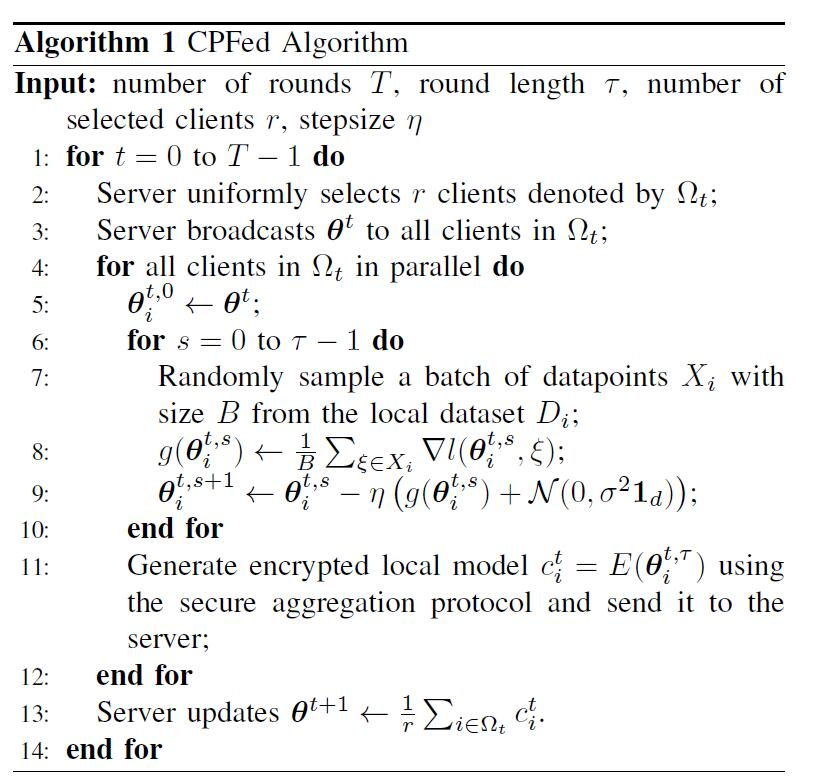
\includegraphics[width=0.7\textwidth]{CPFed/CPFed_Algorithm.jpg}
    \label{CPFed_algorithm}
\end{figure}

CPFed由$T$轮通信迭代组成,每一轮迭代选择一组客户机$\Omega_t$, 其数据集为$\mathcal{D}_i$使用\ref{local_iter}进行$\tau$次局部迭代, 其中每组客户机每轮进行初始化共同的模型. $\tau$轮局部迭代后, 客户机组$\Omega_t$上传加密模型$E(\theta_i^{t,\tau})$,服务器对这些加密信息进行聚合.

\subsection{隐私分析}

\paragraph{Corollary推论1} 第$t-th $轮的第$s$次局部迭代时, 客户$i$的随机梯度$g(\theta_i^{t,s})$的灵敏度以$2L/B$为界. 

\paragraph{Lemma 4 } 
上传的本地模型总和的敏感度$\sum_i \in \Omega_t \theta^{t, \tau}_i$
以$2 \eta \tau L/B$为界. 

通过Lemma 1和4, 可得每轮的zCDP保证

\begin{theorem}
如果算法1中的高斯噪声$b_i^{t,s}$取样与$N(0, \sigma^2 \mathbb{1}_d)$
, 那么算法1经过T轮可以为每个客户机达到$(\epsilon,\delta)-DP$, 其中 
\begin{equation}
    \epsilon = \frac{2T\tau L^2}{n B^2 \sigma^2}+ 2 \sqrt{\frac{2T\tau L^2 }{nB^2\sigma^2} \log\frac{1}{\delta}} 
\end{equation}
\end{theorem}

\subsubsection{收敛性分析}

\begin{figure*}[!ht]
    \setlength{\abovecaptionskip}{0.1cm}
    \centering    
    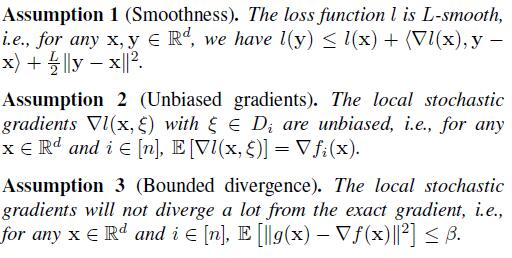
\includegraphics[width=0.7\textwidth]{CPFed/Assumption123.jpg}
    \label{assumption123}
\end{figure*}

假设2中, 无偏差梯度保证随机梯度算法的随机性不影响结果的准确性. 
假设3保证局部随机梯度相差在一定范围内, 即忽略一些客户机偏离正常值
过远的梯度数据. 这些都是联邦学习的常见假设. 
由假设2和假设3, 便可得出引理5: 局部随机梯度的方差有界, 且与精确梯度相差不大.



\begin{figure*}[!ht]
    \setlength{\abovecaptionskip}{0.1cm}
    \centering    
    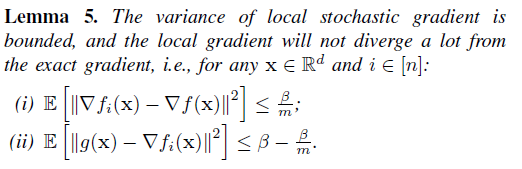
\includegraphics[width=0.7\textwidth]{CPFed/Lemma5.png}
    \label{Lemma5}
\end{figure*}
\newpage
\subsubsection{虚拟更新规则}

定义$\Theta^k, G^k,B^k \in \mathbb{R}^{d \times n} \text{其中} k =0, \dots  K$连接所有局部模型, 梯度, 和噪音
\begin{figure*}[!ht]
    \setlength{\abovecaptionskip}{0.1cm}
    \centering    
    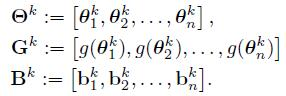
\includegraphics[width=0.4\textwidth]{CPFed/virtualUpdate.jpg}
    \label{virtualUpdate}
\end{figure*} 

\begin{figure*}[!ht]
    \setlength{\abovecaptionskip}{0.1cm}
    \centering    
    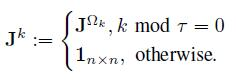
\includegraphics[width=0.5\textwidth]{CPFed/Jk.jpg}
    \label{Jk}
\end{figure*}

\textbf{连接?}


$k \mod \tau =0$意思是每轮迭代结束,进行平均,其余迭代时$J^k= 1_{n \times n} $表示该值无影响.
CPFed 的一般更新规则可以表示为

$$ \Theta^{t+1} =( \Theta ^k - ]eta ( G^k+B^k)) J^k$$

第$k$次迭代的平均模型可表示为

$$ \frac{\Theta^{k+1} \mathbf{1}^k}{r} =\frac{\Theta^k \mathbf{1}^k}{r}- \eta (\frac{G^k \mathbf{1}^k}{r} +\frac{B^k\mathbf{1}^k}{r} )$$


\textbf{安全聚合不会更新本地模型的总和}.

上式可重写为
\begin{figure*}[!ht]
    \setlength{\abovecaptionskip}{0.1cm}
    \centering    
    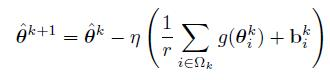
\includegraphics[width=0.6\textwidth]{CPFed/equation16.jpg}
\end{figure*}

\begin{figure*}[!ht]
    \setlength{\abovecaptionskip}{0.1cm}
    \centering    
    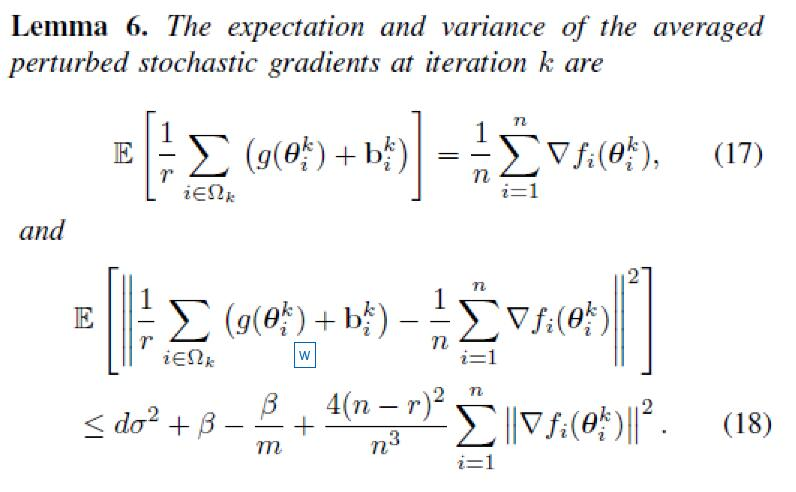
\includegraphics[width=0.7\textwidth]{CPFed/Lemma6.jpg}
    \label{Lemma6}
\end{figure*}

\begin{theorem}
(凸损失的CPFed收敛性)
对于CPFed算法, 假设迭代总次数为$K= T\tau$的次数, 其中$T$为通信轮数, 而n为轮长. 在假设1-4的条件下, 如果学习率满足$5\eta L +20 \tau ^2\eta^2 L^2 \leqslant 1$, 并且所有的客户端初始化在同一个点 $\theta ^0 \in \mathbb{R}^d$, 那么经过K次迭代后, 期望最优性间隙有界如下:
\begin{equation}
  \mathbb{E} \left[  \frac{1}{K} \sum_{k=0}^{K-1}f(\theta^k)-f^\star \right]\leqslant
  \frac{(1-n\lambda)}{K \eta \lambda}  (f(\theta^0)-f^\star (1-n)
  +H(\tau,\sigma^2)
\end{equation}
,其中$H(\tau,\sigma^2) := \eta L /2 \lambda (4 \eta L(\eta L(\tau -1)(2 \tau-1)+1) (d \sigma^2+\beta - \beta /m ))$, $\xi^2$为小批量随机梯度的方差界, 其中, $\sigma^2$为高斯噪声的方差, L为梯度的Lipschitz常数, $\lambda$ 是为强凸性常数, m为局部数据集的大小

\end{theorem}

\begin{theorem}
(CPFed对非凸损失的收敛性). 
对于CPFed算法, 设总送代次数$K=T\tau$, 其中$T$为通信轮数, 而$d$为轮长. 
在假设1-3的条件下, 如果学习率满足$5\eta L +20 \tau ^2\eta^2 L^2 \leqslant 1$, 并且所有的客户端初始化在同一个点 $\theta ^0 \in \mathbb{R}^d$, 那么经过K次迭代后, 期望最优性间隙有界如下:
\begin{equation}
  \mathbb{E} \left[  \frac{1}{K} \sum_{k=0}^{K-1}f( \| \hat{\theta}^k) \|^2  \right]\leqslant 
  \frac{2(f(\theta^0)- f^\star)}{ \eta K} + P(\tau, \sigma^2) 
\end{equation}
, 其中$P(\tau,\sigma^2) := \eta L /2 \lambda (4 \eta L(\eta L(\tau -1)(2 \tau-1)+1) (d \sigma^2+\beta - \beta /m ))$, $\xi^2$为小批量随机梯度的方差界. 其中, $\sigma^2$为高斯噪声的方差, L为梯度的Lipschitz常数, m为局部数据集的大小.
\end{theorem}   



%具体证明另外手写.

\subsection{实验}

\subsubsection{实验装置}
\paragraph{数据集} Adult dataset 48842个样本 14个数字特征(年龄,阶级,种族,性别等)和分类特征(收入). 原始数据分配给16台设备.
\paragraph{学习任务} 训练一个逻辑回归分类器和一个3层神经网络分类器(使用ReLU激活函数)

\paragraph{基准} DP-SGD, 在 DP-SGD中, 每个设备在每个集聚阶段只进行一步随机梯度下降对局部模型进行更新, 每次更新模型时加入高斯噪声后再发送. 

\paragraph{超参数} 80\%的数据用于训练,10\%用于测试,10\%用于验证. Lipschitz常数设为1, 隐私失效概率$=10^{-4} $客户端数$r=10$.

\subsubsection{CPFED的收敛性}
实验参数

逻辑回归
$ \sigma = {10^{-5},10^{-4},10^{-3}}, \tau=\{1,5,10,40\}$
神经网络 
$ \sigma = {10^{-4},10^{-3},5 \times 10^{-3},10^{-3}}, \tau=\{1,5,10,40\}$

\begin{figure*}[!ht]
    \setlength{\abovecaptionskip}{0.1cm}
    \centering    
    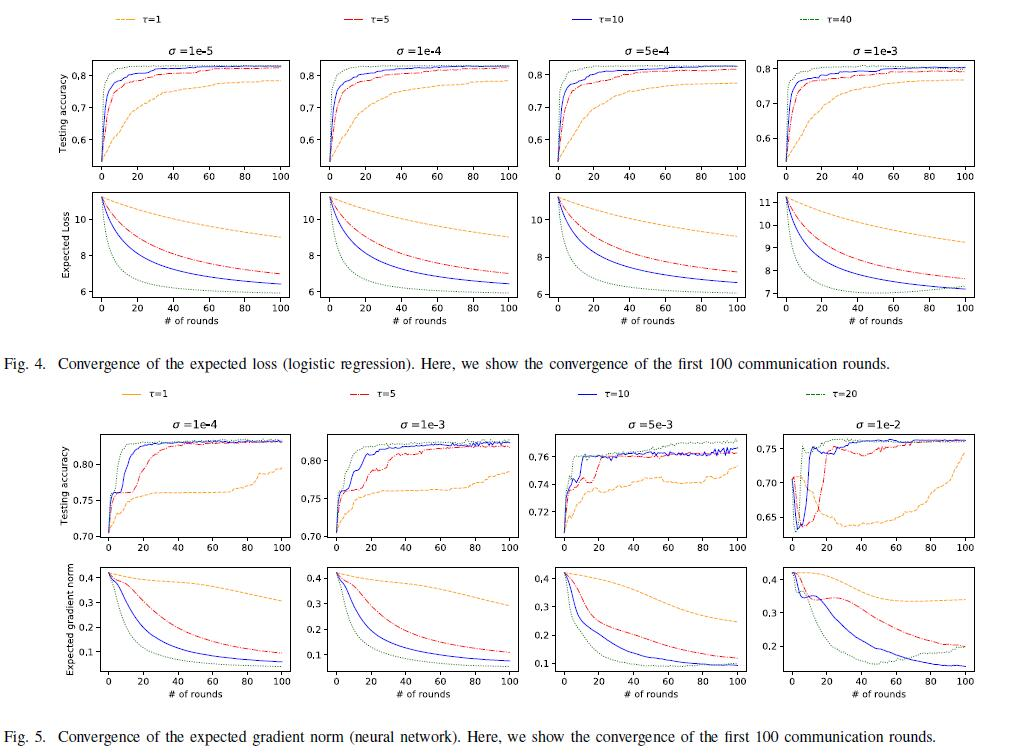
\includegraphics[width=\textwidth]{CPFed/experiment45.jpg} first proposed the concept of deep learning with differential privacy (DP), providing an evaluation criterion for privacy guarantees
\end{figure*}

\begin{figure*}[!ht]
    \setlength{\abovecaptionskip}{0.1cm}
    \centering    
    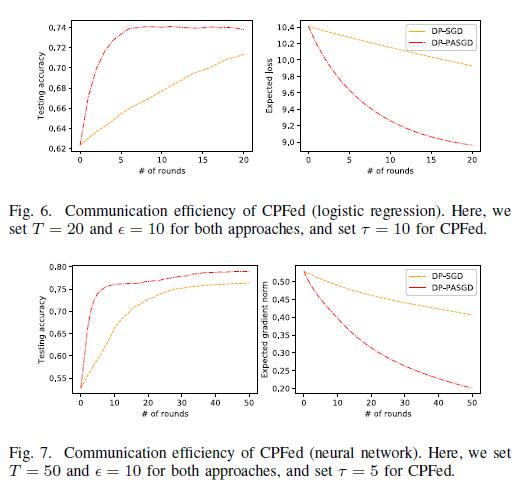
\includegraphics[width=0.8\textwidth]{CPFed/experiment67.jpg}
\end{figure*}

对于logistic回归分类器, 测试准确率和预期损失一般会先急剧下降后缓慢下降. 随着噪声级的增大, logistic回归的期望训练损失收敛到一个更高的界, 测试精度下降, 这与CPFed的收敛特性一致, 其中, 较大的噪声级(index)意味着较大的收敛误差. 对于所有的噪声设置, 随着局部送代次数的增加, 预期损失在开始时下降的更剧烈, 并且到达一个更高的平稳点, 这与CPFed的收敛特性一致, 即较大的收敛系数意味着较大的收敛误差. 

神经网络分类器也有类似的趋势. 当$\sigma=10^{-2}$时当噪声进入系统时, 测试精度会从初始值迅速下降, 然后随着计算量和通信量的增加而增加. 说明加噪声过大影响精确度.

\paragraph{通信效率比较} CPFed与基准方法DP-SGD的通信效率进行比较, CPFed比DP-SGD收敛更快, 比DP-SGD获得更高的精度和更低的期望梯度范数. 无论在凸还是非凸情况下, CPFed都比DP-SGD实现了更高的通信效率. 因为CPFed可以在多台机器上进行多步梯度更新,模型能更快收敛.


% \section{Performance Analysis and Optimization in Privacy-Preserving Federated Learning}


\subsection{背景}

\subsubsection{挑战}

在FL中, 敌人可能会通过窃听和分析共享参数来攻击学习模型(重构攻击和推理攻击). 
例如, 恶意分类器可能揭示客户数据的特征, 并根据给定的FL模型重构数据点.  

超大数据量和隐私保护的要求下,联邦学习(FL)得到应用. 由于FL本地训练, 不要求客户上传他们的私人数据, 因此有效地减少了传输开销, 同时保护客户的隐私. 
因此, FL 适用于各种数据敏感或传输到服务器代价昂贵的情况, 例如, 医疗记录、私人图像和个人识别信息等. 
虽然 FL 可以保护私有数据不被公开, 但是 共享参数可能被窃取用来分析攻击模型(例如重构攻击和推理攻击). 

\paragraph{本文贡献}

利用本地差分隐私(Local DP), 引入客户端级别差分隐私(CDP)算法 

证明CDP在一定隐私水平下满足DP的要求,求出了CDP的理论收敛界.
 

\subsection{相关工作}
\begin{itemize} 
    \item Privacy-Preserving Deep Learning  \cite{shokri2015privacy}表明集中搜索数据仓库和开放数据应用的出现可能会导致私人信息的泄露. 
    % \item Deep Learning with Differential Privacy \cite{abadi2016DLwithDP}首次提出了差分隐私深度学习(DP)的概念, 为隐私保障提供了评价标准
    \item Privacy-Preserving Collaborative Deep Learning With Unreliable Participants  \cite{zhao2020collaborative}设计了一种函数机制, 在训练过程中扰动神经网络的目标函数, 以达到一定的DP水平
    \item Concentrated Differentially Private Gradient Descent with Adaptive per-Iteration Privacy Budget \cite{Lee2018ConcentratedDP}  改进了基于DP的随机梯度下降(SGD)算法, 在每次训练迭代中仔细分配隐私预算. 
    \item Differentially Private Distributed Online Learning \cite{Li2018DiffOnline}  引入数据处理的概念, 提出了一种分布式在线学习算法, 以提高在给定隐私水平下的学习性能
    \item Differentially Private Federated Learning: A Client Level Perspective \cite{Geyer2017Client} 提出了一个保护隐私的FL框架, 当有足够多的客户参与时, 可以在低性能损失的情况下保持一个给定的隐私水平. 
    \item A Hybrid Approach to Privacy-Preserving Federated Learning\cite{Truex:2019:HAP:3338501.3357370} 将DP与安全多方计算相结合 
    \item Privacy for Free: Communication-Efficient Learning with Differential Privacy Using Sketches \cite{li2019privacy}  提出基于sketches草图的FL框架, 为客户获得可证明的DP好处, 它可以将通过草图传输的消息压缩到很高的通信效率. 
    
草图算法(sketch)在数据集上提供不同统计数据(如计算不同的计数或平均值)的近似估计,并被广泛应用于流数据处理、数据库和网络测量。
草图也被用于大规模机器学习,如压缩模型更新,识别梯度向量中的重要坐标,减少模型训练中的内存使用。

最近, 的一些尝试考虑通过使用随机噪声、随机采样或其他随机方法来扩展草图,以提供差分隐私。
但是,他们需要在草图之上添加这些机制,并且不研究草图本身的任何固有的隐私属性。
分析表明,草图具有固有的不同的隐私属性,可以用于设计私有分布式学习算法,与最先进的机制相比,该算法能够实现更好的通信和准确性权衡
     
\end{itemize}

    以上工作提出了差分隐私, 给出隐私性能评价标准, 给出了设置一定隐私水平的目标函数的方法, 并利用分布式在线学习, 安全多方计算, Sketches 等方法概念, 提高联邦学习的计算性能隐私性能和通信效率. 

  
Calibrating Noise to Sensitivity in Private Data Analysis\cite{Dwork2006} 提出了根据敏感度来添加噪声实现差分隐私的方法. 证明可以通过根据函数f的灵敏度来校准噪声的标准偏差来保持隐私. 粗略地说, f的任何一个参数可以改变其输出的量. 


    下表\ref{tab:FLnotation}表示了本文常用的符号.
    \begin{figure}[!ht]
        \centering
        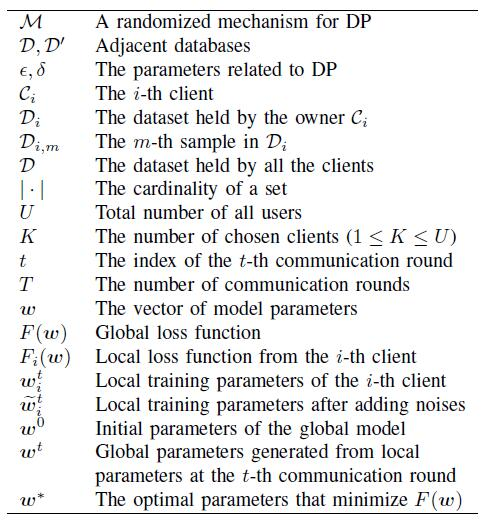
\includegraphics[width=0.6\textwidth]{CDP/notation.jpg}
        \caption{主要符号}
        \label{tab:FLnotation}
    \end{figure}
\subsection{预备知识}

 

\subsubsection{本地差分隐私}

传统的差分隐私是将原始数据集中到一个数据中心, 然后在此对数据施加差分隐私算法, 并对外发布, 称之为中心化差分隐私(Centralized Differential Privacy). 因此, 中心化差分隐私有一个前提: \textbf{可信的第三方数据收集者}, 即保证所收集的数据不会被窃取和泄露. 然而, 在实际生活中想找到一个真正可信的第三方数据收集平台十分困难, 这极大地限制了中心化差分隐私的应用. 

未解决以上问题本地化差分隐私,  基于不可信第三方的前提下, 其将数据隐私化的工作转移到每个用户, 用户自己来处理和保护个人数据, 极大地降低了隐私泄露的可能性. 
任意本地化差分隐私函数f, 定义域为$Dom(f)$, 值域为$Ran(f)$, 对任意输入$t, t^{'} \in Dom(f)$, 输出$t^{*} \in Ran(f)$, 都有:

$P[ f(t) = t^{*} ] \leq e^{\varepsilon }\times P[ f(t^{'}) = t^{*} ] $

本地化差分隐私技术通过控制任意两条记录的输出结果的相似性, 从而确保算法f满足本地化差分隐私, 即输出同为$t^{*}$, 窃密者无法确认输入为$t$还是$t^{'}$;
$\varepsilon$越小, 任意两条记录输出结果相似性越高. 

\begin{figure}[!ht]
    \caption{本地差分隐私}
    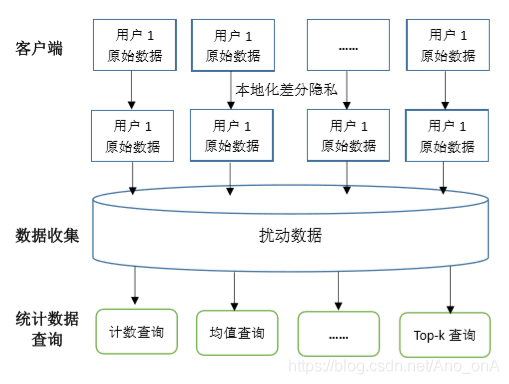
\includegraphics[width=0.8\textwidth]{CDP/LDP.png}
\end{figure}

\paragraph{Client Level Differentially Privacy }
(集中式)联邦学习情况下,受信任的管理者会聚合由多个客户以分散方式优化的参数。然后,产生的模型被分发回所有的客户端,最终在不显式共享数据的情况下汇聚成一个联合的代表模型。但是,该协议很容易受到不同攻击,这些攻击可能来自在联邦优化期间参与的任何一方。在这样的攻击中,通过分析分布式模型,客户在训练中的贡献和他们数据集的信息被揭示出来。针对这一问题,\cite{Geyer2017Client}提出了一种客户端差分隐私保护联邦优化算法。其目的是在训练期间隐藏客户的贡献,平衡隐私损失和模型性能之间的权衡。实证研究表明,如果\textbf{有足够多的参与客户,其提出的程序可以在模型性能上以很小的成本保持客户级别的差分隐私。}

\paragraph{该文的主要贡献:}在联邦学习中保持较高的模型性能时,可以隐藏客户的参与, 在轻微损失模型的性能下实现客户端级别差分隐私。
其次,提出在分布式训练中动态适应dp保护机制。 与集中式学习相比,联邦学习中的梯度在整个训练过程中对噪音和批量大小表现出不同的灵敏度。
\cite{McMahan2018Learning}提出了一个类似的客户级dp程序。不同的是其实验设置\cite{McMahan2018Learning}还包括元素级隐私措施。
\textbf{元素级隐私}

\paragraph{方法}
\begin{enumerate}
    \item \textbf{Random sub-sampling随机子抽样}
    \item \textbf{Distorting:} A Gaussian mechanism is used to distort the sum of all updates. This requires knowledge about the set’s sensitivity with respect to the summing operation. We can enforce a certain sensitivity by using scaled versions instead of the true updates:$w^t_i=max(1, \|  \frac{w^t_i}{S}\|)$. Scaling ensures that the second norm is limited $\forall k, \|w^t_i\|_2<S$. The sensitivity of the scaled updates with respect to the summing operation is thus upper bounded by S. The GM now adds noise (scaled to sensitivity S) to the sum of all scaled updates. Dividing the GM’s output by mt yields an approximation to the true average of all client’s updates, while preventing leakage of crucial information about an individual.

   缩放后的更新相对于求和运算的灵敏度因此上限为S。高斯机制将噪声(缩放到灵敏度S)加到所有缩放后的更新的和上。 
\end{enumerate}

\leader{R\'enyi Divergence}
\begin{definition}[{R\'enyi Divergence ]{ }}]
    Let $P$ and $Q$ be probability distributions on $\Omega$. For $\alpha \in  (1,\infty)$, we define the \emph{R\'enyi divergence of order $\alpha$ between $P$ and $Q$} as 
    \begin{align*}
    D_\alpha (P||Q)
     =& \frac{1}{\alpha - 1} \log \left( \int_\Omega P(x)^\alpha Q(x)^{1-\alpha} \mathrm{d} x \right) \\
     =& \frac{1}{\alpha-1} \log \left( \ex{x \sim Q}{ \left(\frac{P(x)}{Q(x)}\right)^\alpha} \right) \\
     =& \frac{1}{\alpha-1} \log \left( \ex{x \sim P}{ \left(\frac{P(x)}{Q(x)}\right)^{\alpha-1}} \right),
    \end{align*}


其中$P(\cdot)$ and $Q(\cdot)$ 分别是$P$和$Q$的概率质量/密度函数. 更一般地, $P(\cdot)/Q(\cdot)$ 是  $P$对于$Q$的Radon-Nikodym导数.\footnote{If $P$ is not absolutely continuous with respect to $Q$ (i.e. it is not the case that $P \ll Q$), we define $D_{\alpha}({P}||{Q})=\infty$ for all $\alpha \in [1,\infty]$.}

 
我们定义 KL-divergence $$\dr{1}{P}{Q} = \lim_{\alpha \to 1} \dr{\alpha}{P}{Q} = \int_\Omega P(x) \log \left(\frac{P(x)}{Q(x)}\right) \mathrm{d}x$$ 和 max-divergence $$\dr{\infty}{P}{Q} = \lim_{\alpha \to \infty} \dr{\alpha}{P}{Q} = \sup_{x \in \Omega} \log \left(\frac{P(x)}{Q(x)}\right) .$$

 R\'enyi divergence 可以被定义为$P$ 和 $Q$隐私损失  : $$e^{(\alpha-1)\dr{\alpha}{P}{Q}} = \ex{Z\sim\privloss{P}{Q}}{e^{(\alpha-1)Z}}$$ for all $\alpha \in (1,\infty)$. 而且, $\dr{1}{P}{Q} = \ex{Z\sim\privloss{P}{Q}}{Z}$.

    \end{definition}


\leader{计算S值} 

在每个通信轮中,计算所有未剪切梯度贡献的平均值,并使用它作为剪切界$S=median{\triangle w^k}_{k \in \mathbf{Z}_t}$. 

\subsubsection{威胁模型--需应对的问题}
\textbf{推理攻击}通过模型推断私有特征和\textbf{重构攻击}通过模型重构训练数据
在重构攻击中, 攻击者的目标是推断训练集中记录的属性. 
推理攻击中, 攻击者的目标是推断特定的个人数据记录是否包含在训练数据集中. 
\paragraph{本文假设}服务器诚实但好奇.即敌手诚实地遵守协议, 但也会试图从接受到的信息中学习除输出意外的信息. 

如下图\ref{fig:threatModel}所示,一个有诚实但好奇的服务器或窃听者的FL训练模型, 他们可以通过分析来自客户端的训练参数来推断私有特征并重建原始数据. 

\begin{figure}[!ht]
    \centering
    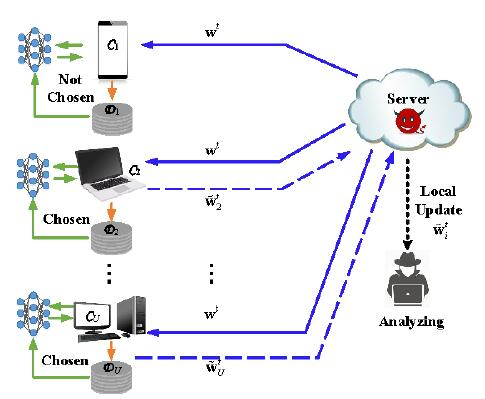
\includegraphics[width=0.5\textwidth]{CDP/threat.jpg}
    \caption{threat model}
    \label{fig:threatModel}
\end{figure}

\subsection{隐私和收敛性分析}


\subsubsection{Client-level DP 客户端级别DP}

\begin{figure}[!ht]
    \centering
    \includegraphics[width=0.6\textwidth]{CDP/alg_CDP.jpg}
    \caption{客户端级DP算法CDP}
    \label{fig:alg_CDP}
\end{figure}
其中,$T$表示通信轮数, $w^0$为初始化全局参数, $\sigma$为加性噪音的标准方差, q为随机抽样比率$K=| \mathcal{K}= qU|$. 

初始: 服务器向客户机初始化全局参数$w^0$

第t轮聚合: K个客户端完成$w$的局部训练, 利用阈值C进行裁剪, 向$w_i^{t+1}$增加噪音得到参数$\tilde{w}_i^{t+1}$并上传. $\tilde{w}_i^t=w_i^t + \mathcal{N}(0, \sigma^2I)$. 
之后,服务器更新全局参数$w^{t+1}$, 并广播. 客户端利用局部数据测试准确率并开始下一轮循环.
直至通讯轮数达到$T$.

\subsubsection{Bound of the Moment}
根据~\cite{abadi2016DLwithDP}, 使用高斯机制, 我们可以定义隐私损失
\begin{equation}
c \triangleq \exp\left(\alpha^{T}(\lambda)\right) = \exp\left(\sum_{t=1}^{T}\alpha(\lambda)\right),
\end{equation}
和矩生成函数
\begin{equation}
\alpha(\lambda) \triangleq \ln(\max \{D_{\nu_{1},\nu_{0}}, D_{\nu_{0},\nu_{1}}\}),
\end{equation}
其中$\lambda$ 是任意正整数, $\nu_{0}$ 为 $\mathcal{N}(0,\sigma^{2})$的概率密度函数(PDF), $\nu_{1}$ 表示 两个高斯分布 $q\mathcal{N}(\Delta s,\sigma^{2})+(1-q)\mathcal{N}(0,\sigma^{2})$的复合, $q=K/U$ 是随机取样率,
\begin{equation}
D_{\nu_{1},\nu_{0}}=\mathbb{E}_{z\sim \nu_{1}}\left(\frac{\nu_{1}}{\nu_{0}}\right)^{\lambda}=\mathbb{E}_{z\sim \nu_{0}}\left(\frac{\nu_{1}}{\nu_{0}}\right)^{\lambda+1},
\end{equation}
and
\begin{equation}
D_{\nu_{0},\nu_{1}}=\mathbb{E}_{z\sim \nu_{0}}\left(\frac{\nu_{0}}{\nu_{1}}\right)^{\lambda}=\mathbb{E}_{z\sim \nu_{0}}\left(\frac{\nu_{1}}{\nu_{0}}\right)^{-\lambda}.
\end{equation}

%We will use moments accountant method to keep track of a bound on the moments with random sampling. This method can provide a much tighter estimation of the privacy loss.

然而, ~\cite{abadi2016DLwithDP}中关于矩界的推导只能应用于严格约束$q \leq \frac{1}{16\sigma}$. 
为了解决这个问题, 我们提出~\textbf{Lemma~\ref{lemma:Comp_div}}来进一步约束该矩. 
\begin{lemma}

考虑到moments accountant法中使用的两种高斯分布$\nu_{0}$和$\nu_{1}$, 它们满足以下关系: 
\begin{equation}
D_{\nu_{1},\nu_{0}}\geq D_{\nu_{0},\nu_{1}}.
\end{equation}
\end{lemma}


\begin{figure}
    \includegraphics[width=0.9\textwidth]{figures/CDP/moment_bound.jpg}
\end{figure}

Privacy accounting:对于不同隐私的SGD来说, 一个重要的问题是计算训练的总体隐私成本. 不同隐私的可组合性使我们能够实现一个“accountant”程序, 计算每次访问训练数据时的隐私损失, 并累积这些成本. 
\cite{abadi2016DLwithDP, mcsherry2009privacy}
 
\subsubsection{敏感度和隐私分析}

相邻数据集:我们在第i个用户中考虑两个相邻的数据库$D_i, D_i^\prime \in\mathcal{X} $, 其中$Di$和$D0i$大小相同, 只相差一个样本. 
实值函数的敏感度可以表示为由于添加或删除单个样本,  函数值可能发生变化的最大程度. 
 
在本文中, 我们选择了采用$L_2$范数灵敏度的高斯机制, 函数$s$的灵敏度可以表示为
\begin{equation}
\Delta s = \max\Vert s(\mathcal D)-s(\mathcal D')\Vert_{2}.
\end{equation}
 
\paragraph{局部敏感度} 对于一个查询函数f , 它的形式为: $f : D \to \mathbb{R}$ , 其中D为一数据集, R 是查询函数的返回结果。在一给定的数据集D 和与它相邻的任意数据集$D'$上, 它的局部敏感度定义如下:

$LS_f=\max_{D'} \|f(D)-f(D')\|$

与全局敏感度不同, 局部敏感度是由查询函数和给定的数据集共同决定, 因为局部敏感度只是对于一个数据集做变化。因为局部敏感度限制了一对相邻数据集中的一个数据集, 所以如果在局部敏感度中, 给定的数据集和全局敏感度中使$\|f(D)-f(D')\|$达到最大的数据集相同时, 局部敏感度等于全局敏感度. 


\begin{assumption}
    假设局部训练中的批量大小等于训练样本的数量. 
    \label{assump1}
\end{assumption}


基于\ref{assump1},用梯度下降法,
\begin{figure}[!ht]
    \centering
    \includegraphics[width=0.6\textwidth]{CDP/generalGD.jpg}
\end{figure}
得到敏感度
$ \triangle l = \frac{2C}{D_i}$, 其中C是阈值.


\begin{theorem}
    给定采样比q和通信轮数T,保证$(\varepsilon, \delta)-DP$对于训练数据集中使用的所有数据, 高斯机制噪声扰动的STD应该满足
$$\sigma= \frac{\sqrt{2qT\ln(1/\delta)} }{\varepsilon}$$
\end{theorem}

 将等式21换为20, 有$\sigma^{t+1}= \sigma^t$.

 CRD算法可以总结为以下
\begin{assumption}
    \begin{figure}[!ht]
        \centering
        \includegraphics[width=0.7\textwidth]{CDP/assump2.jpg}
    \end{figure}
\end{assumption}

\begin{theorem}
    \label{theorem2}
    \begin{figure}[!ht]
        \centering
        \includegraphics[width=0.8\textwidth]{CDP/theorem2.jpg}
    \end{figure}
\end{theorem}
理论\ref{theorem2} 显示了收敛性能和隐私之间的精确权衡:当隐私保证较弱时,收敛边界较小, 表明收敛到最优权值的收敛. 从我们的假设中, 我们知道$\eta L  \leqslant 1, \ A <1 $.


\subsection{CDP中的折扣DISCOUNTING方法}

当训练性能停止提高时,稍微降低T的值,可以得到更小的STD,从而提高性能. 
据此,作者提出CRD算法(communication rounds discounting). 在CRD中, T是迭代确定的. 如图\ref{fig:alg_CDP}所示,表现了带CRD的CDP算法在第t轮通信的训练过程.

步骤1, 初始化: 服务器广播$w^0$初始参数,$T, \upsilon \text{和}\delta$;

步骤2, 局部训练

步骤3, 梯度剪裁: 为了证明DP保证,每个例子对当地的影响参数应与限幅阈值有界c.每个参数向量将在L2范数范围内. 如第i个局部参数向量$w^t_i$在第t轮沟通被$w^t_i=max(1, \|  \frac{w^t_i}{C}\|)$替换(这种参数剪裁形式在SGD和ML常用.
由于差分隐私保护要求限制每个样本对最终梯度$\tilde{g}_t$的影响。鉴于梯度的取值范围无先验
限定,故采用$L_2$范数首先对每个梯度进行裁剪, 
裁剪后结果为:若$\|g\|_2 \leq C$,则保留g,若$\|g \|_2 > C$,则将其缩小为常量C。进行隐私损失累积操作的主要目的在于跟踪计算每次训练迭代过程中的隐私损失成本。可以根据所加噪声的分布参数进而确定每次叠加过程的隐私损失$α(\delta)$。

步骤4, 添加噪声: 具有确定STD的人工高斯噪声将被添加到本地训练参数保证$(\upsilon,\delta)-\text{DP}$; 本地参加噪声区别于中心化差分隐私.
步骤5, 参数上传

步骤6, 模型聚合

步骤7, 模型广播: 服务器广播聚合的参数和通信轮数T给所有客户端;

步骤8,模型更新:所有客户更新各自与聚合模型参数,然后测试的性能更新模型和性能上传到服务器;

步骤9:通信轮折扣:当停止提高收敛性能, 服务器的折现方法将被触发. 服务器将获得一个小于前一个T的线性折扣因子. 这个因素可以控制T的衰减速度, 当聚合时间达到预设的T时, 联邦学习过程结束. 

  

梯度范数剪切阈值的选取需要综合考虑如下两个因素:1) 若阈值取值过小,则最终以平均值代替真实梯度时可能造成误差过大;2) 若阈值取值过大,则由算法1 可知,将会导致最终根性的梯度中注入过多的噪声。
\begin{figure}[!ht]
    \centering
    \FloatBarrier
    \includegraphics[width=0.8\textwidth]{CDP/CRD.jpg}
    \caption{使用CRD方法训练CDP第t轮通信中过程}
    \label{CRD}

\end{figure}
 

\subsubsection{T的噪声重计}

\begin{theorem}
    \label{theorem3}
    \begin{figure}[ht]
        \centering
        \includegraphics[width=0.8\textwidth]{CDP/theorem3.jpg}
    \end{figure}
\end{theorem}

基于前面的训练过程和T的值, 我们可以获得一个有合适的STD的噪声. ($\sigma^\tau$小)
如果在前面的训练过程有较大STD(强隐私保证), 重新计算后的STD将小(弱隐私保证).($\sigma^t$小)
如果在这轮通信中T的值不变, 那么STD的值将保持不变. 
考虑$\sigma^t, \sigma^{t+1}$和不变的T,从上面的方程,可得
\begin{figure}[!ht]
    \centering
    \includegraphics[width=0.6\textwidth]{CDP/equation2021RecalT.jpg}
\end{figure} 

\begin{figure}[ht]
    \includegraphics[width=0.7\textwidth]{CDP/alg_code_CRD.jpg}
    \label{alg_code_CRD}
    \caption{CDP with CRD method}
\end{figure}
    在\ref{alg_code_CRD}中,有CRD方法的详细步骤.

\subsection{实验}
\subsubsection{结果评价}

\begin{figure}[ht]
    \centering
    \includegraphics[width=3.2in,angle=0]{figures/CDP/Svm_ConvforNandK_T.pdf}
    \caption{Value of the loss function under various $T$ using the CDP algorithm (SVM). (a) $U=50, K=50$ ($q=1$). (b) $U=50, K=30$ ($q=0.6$).}
    \label{fig:SVM_ConvforNandK_T}
    \end{figure}

    \begin{figure}[ht]
    \centering
    \includegraphics[width=3.2in,angle=0]{figures/CDP/ConvforKandN_T.pdf}
    \caption{Value of the loss function under various $T$ using the CDP algorithm (MLP). (a) $U=50, K=50$ ($q=1$). (b) $U=50, K=30$ ($q=0.6$).}
    \label{fig:MLP_ConvforNandK_T}
    \end{figure}

    \begin{figure}[ht]
    \centering
    \includegraphics[width=3.2in,angle=0]{figures/CDP/ConvforN_T_eps_td.pdf}
    \caption{Value of the loss function under various $T$ and privacy levels using the CDP algorithm (MLP) with $U=K=50$ ($q=1$).}
    \label{fig:ConvforN_T_eps_td}
    \end{figure}

    \begin{figure}[ht]
    \centering
    \includegraphics[width=3.2in,angle=0]{figures/CDP/ConvforK_T_eps_td.pdf}
    \caption{Value of the loss function under various $T$ and privacy levels using the CDP algorithm (MLP) with $U=50$ and $K=30$ ($q=0.6$).}
    \label{fig:ConvforK_T_eps_td}
    \end{figure}
    Fig~\ref{fig:ConvforN_T_eps_td}和~\ref{fig:ConvforK_T_eps_td} 用来说明抽样的作用.

Fig~\ref{fig:ConvforN_T_eps_td}和~\ref{fig:ConvforK_T_eps_td}通过改变隐私级别$\epsilon$和$T$的值, 说明了使用MLP模型在FL中的CDP算法训练损失函数值的期望. 从图~\ref{fig:ConvforN_T_eps_td}可以看出, 没有采样, 较大的$T$和较小的$\epsilon$性能糟糕. 如图~\ref{fig:ConvforN_T_eps_td}中采样比$q=0.6$的第二种情形所示, 它也可以保持同样的性质. 

抽样和批量随机梯度下降法类似.
作者用SVM和MLP模型来验证理论结果.  观察结果与Remark 1 一致, 其因为较低的隐私水平降低了附加噪声的标准差, 服务器可以从客户端获得更好质量的ML模型参数. 从 \ref{fig:SVM_ConvforNandK_T} 和图\ref{fig:MLP_ConvforNandK_T} 中,可以看出T的最优值几乎随着$\varepsilon$的增加而增加. 

 
\subsubsection{对CRD的评价}
\paragraph{T初始化}
当T更接近T的最优值时, 会得到更好的收敛性能.
\paragraph{隐私级别}
更小的隐私水平使用CRD方法更早结束. T越大, 信息泄漏的可能性越大, 附加噪声的STD越大. 之后, CRD方法可能被触发, 减小的T将从服务器广播到客户端. 
\paragraph{折扣因子} 当隐私级别固定时, 较大的$\beta$会导致T较慢的衰减速度,意味着在训练中仔细调整T有利于收敛性能. 更仔细的调整将导致更多的通信回合消耗. 最优CDP具有最好的收敛性能, 但需要消耗大量的通信轮数. 最终结论:通过选择多路切换, 在通信周期消耗和收敛性能之间存在一个折衷.  
\textbf{未来待研究:解析地评估损失函数最小的最优值. }

\subsection{结论}
本文为解决联邦学习训练中防止共享参数被窃取导致隐私泄露的情况, 设计CDP算法保护隐私, 并进一步通过折扣法提高训练效率, 且从理论上得出该算法的上界. 最后根据实验评价通信轮数T, 隐私水平参数 $\varepsilon$, 折扣因子$\beta$对算法的影响. 
算法重点如下:
引入本地差分隐私, 根据灵敏度得到剪切阈值,并据此设计满足$(\varepsilon,\delta)-DP$的加噪高斯机制. 

提出CRD折扣法, 收敛性能稳定时触发该机制, 并自动优化参数T, 并动态更改加噪方差, 进一步获得更优模型. 









 
 


\subsection{公式推导}

\subsubsection{Bound of the Moment 矩界}

\begin{algorithm}[htb]
	\caption{Differentially private SGD (Outline)}\label{alg:privsgd}
	\begin{algorithmic}
	\REQUIRE Examples $\{x_1,\ldots,x_N\}$,\\ loss function $\calL(\btheta)=\frac{1}{N}\sum_i \calL(\btheta, x_i)$. \\ Parameters: learning rate $\eta_t$, noise scale $\sigma$, group size $L$, gradient norm bound $C$. 
%\bmnote{Give a formula for choosing $\sigma_t$. Also: why two Input: (\REQUIRE) lines?}
%LZ: we are adopting the strategy of choosing sigma and then using privacy
%accountant to accumulate the privacy loss. Maybe we should make that more
%explicit in Privacy Accountant section?
		\STATE {\bf Initialize} $\btheta_0$ randomly
		\FOR{$t \in [T]$}
		\STATE {Take a random sample $L_t$ with sampling probability $L/N$}
		\STATE {\bf Compute gradient}
		\STATE {For each $i\in L_t$, compute $\bfg_t(x_i) \gets \nabla_{\btheta_t} \calL(\btheta_t, x_i)$}		
		\STATE {\bf Clip gradient}
		\STATE {$\bar{\bfg}_t(x_i) \gets \bfg_t(x_i) / \max\big(1, \frac{\|\bfg_t(x_i)\|_2}{C}\big)$}
		\STATE {\bf Add noise}
		\STATE {$\tilde{\bfg}_t \gets \frac{1}{L}\left( \sum_i \bar{\bfg}_t(x_i) + \mathcal{N}(0, \sigma^2 C^2 \Id)\right)$}
		\STATE {\bf Descent}
		\STATE { $\btheta_{t+1} \gets \btheta_{t} - \eta_t \tilde{\bfg}_t$}
		\ENDFOR
		\STATE {\bf Output} $\btheta_T$ and compute the overall privacy cost $(\eps, \delta)$ using a privacy accounting method.
%\bmnote{Ref to Eqs or pseudocode for computing privacy cost.}
%LZ: we will spend most of time discussing how privacy is computed. Since
%the algorithm description is an outline, maybe we can postpone it?
	\end{algorithmic}
\end{algorithm}

\begin{theorem}
      \label{thm:momentBound}
	存在常数 $c_1$ and $c_2$ 使 已知抽样概率  $q=L/N$以及步数$T$, 对于任意$\eps < c_1 q^2T$, 如果我们选择以下$\sigma$值, 算法~\ref{alg:privsgd} 对于任意$\delta>0$  是 $(\eps,\delta)$-DP,  
	\begin{align*}
	\sigma \geq c_2\frac{q \sqrt{T \log(1/\delta)}}{\eps}\,.
	\end{align*}
\end{theorem}

根据~\cite{abadi2016DLwithDP}, 使用高斯机制, 我们可以定义隐私损失
\begin{equation}
c \triangleq \exp\left(\alpha^{T}(\lambda)\right) = \exp\left(\sum_{t=1}^{T}\alpha(\lambda)\right),
\end{equation}
和矩生成函数
\begin{equation}
\alpha(\lambda) \triangleq \ln(\max \{D_{\nu_{1},\nu_{0}}, D_{\nu_{0},\nu_{1}}\}),
\end{equation}
其中$\lambda$ 是任意正整数, $\nu_{0}$ 为 $\mathcal{N}(0,\sigma^{2})$的概率密度函数(PDF), $\nu_{1}$ 表示 两个高斯分布 $q\mathcal{N}(\Delta s,\sigma^{2})+(1-q)\mathcal{N}(0,\sigma^{2})$的复合, $q=K/U$ 是随机取样率,
\begin{equation}
D_{\nu_{1},\nu_{0}}=\mathbb{E}_{z\sim \nu_{1}}\left(\frac{\nu_{1}}{\nu_{0}}\right)^{\lambda}=\mathbb{E}_{z\sim \nu_{0}}\left(\frac{\nu_{1}}{\nu_{0}}\right)^{\lambda+1},
\end{equation}
和
\begin{equation}
D_{\nu_{0},\nu_{1}}=\mathbb{E}_{z\sim \nu_{0}}\left(\frac{\nu_{0}}{\nu_{1}}\right)^{\lambda}=\mathbb{E}_{z\sim \nu_{0}}\left(\frac{\nu_{1}}{\nu_{0}}\right)^{-\lambda}.
\end{equation}

%We will use moments accountant method to keep track of a bound on the moments with random sampling. This method can provide a much tighter estimation of the privacy loss.

然而, ~\cite{abadi2016DLwithDP}中关于矩界的推导只能应用于严格约束$q \leq \frac{1}{16\sigma}$. 
为了解决这个问题, 我们提出~\textbf{Lemma~\ref{lemma:Comp_div}}来进一步约束该矩. 
\begin{lemma}\label{lemma:Comp_div}

考虑到矩会计法中使用的两种高斯分布$\nu_{0}$和$\nu_{1}$, 它们满足以下关系: 
\begin{equation}
D_{\nu_{1},\nu_{0}}\geq D_{\nu_{0},\nu_{1}}.
\end{equation}
\end{lemma}

 
Privacy accounting:对于不同隐私的SGD来说, 一个重要的问题是计算训练的总体隐私成本. 不同隐私的可组合性使我们能够实现一个“accountant”程序, 计算每次访问训练数据时的隐私损失, 并累积这些成本. 



\subsection{理论1的证明}
 
差分隐私保证转为moment bound矩界.

\newtheorem{thm_appendix}{Theorem}[section]
\newtheorem{lem_appendix}[thm_appendix]{Lemma}
\begin{lem_appendix}
  \label{lem:pure_dp_to_logmgf}
  Let $\calM$ be $\eps$-differentially private. Then for any $\lambda > 0$, $\calM$ satisfies
\begin{align*}
\alpha_{\lambda} \leq \lambda\eps(e^{\eps}-1) + \lambda^2\eps^2e^{2\eps}/2.
\end{align*}
  \end{lem_appendix}
\begin{proof}
  Let $Z$ denote the random variable $c(\calM(d))$. Then differential privacy implies that
  \begin{itemize}
      \item $\mu \eqdef \E[Z] \leq \eps(\exp(\eps) - 1)$.  
      \item $|Z| \leq \eps$, so that $|Z-\mu| \leq \eps \exp(\eps)$.
    \end{itemize}
  Then $\E[\exp(\lambda Z)] = \exp(\lambda\mu) \cdot \E[\exp (\lambda(Z-\mu))]$. Since $Z$ is in a bounded range $[-\eps\exp(\eps), \eps\exp(\eps)]$ and $f(x) = \exp(\lambda x)$ is convex, we can bound $f(x)$ by a linear interpolation between the values at the two endpoints of the range. Basic calculus then implies that
  \begin{align*}
    \E[f(Z)] \leq f(\E[Z]) \cdot \exp(\lambda^2 \eps^2 \exp(2\eps)/2),
    \end{align*}
 which concludes the proof.
 \end{proof}
\mycomment{Similarly,
\begin{lemma}
  \label{lem:approx_dp_to_logmgf}
  Let $\calM$ be $(\eps,\delta)$-DP. Then $\calM$ is $(\lambda\eps(e^{\eps}-1) + \lambda^2\eps^2e^{2\eps}/2, \delta, \lambda)$-logmgf bounded.
  \end{lemma}
}
 
\setcounter{theorem}{1}\begin{theorem}\label{thm:property_supp}
    Let $\alpha_\calM(\lambda)$ defined as \[\alpha_\calM(\lambda) \eqdef \max_{\aux, d, d'} \alpha_\calM(\lambda; \aux, d, d'),\]
    最大值被接收所有的辅助输入和邻近的数据库$d,d'$,那么有
    
    \begin{enumerate}
    \item \textbf{[Composability]}
    Suppose that a mechanism $\calM$ consists of a sequence of adaptive mechanisms $\calM_1, \ldots, \calM_k$ where $\calM_i\colon \prod_{j=1}^{i-1}\Range_j\times \Domain \to\Range_i$. Then, for any $\lambda$
    \[\alpha_\calM(\lambda) \leq \sum_{i=1}^k \alpha_{\calM_i}(\lambda)\,.\]
    
    \item \textbf{[Tail bound]}
    For any $\eps>0$, the mechanism $\calM$ is $(\eps, \delta)$-differentially private for
    \[\delta=\min_{\lambda} \exp(\alpha_\calM(\lambda) -\lambda \eps)\,.\]
    \end{enumerate}
    \end{theorem}
     

Lemma~\ref{lem:pure_dp_to_logmgf}和Theorem~\ref{thm:property_supp}给出了一种获得差分机制的组合定理的方法,这大致相当于展开~\cite{Dwork2010boosting}的强组合定理的证明。\logmgfa会计的有效性是因为,对于许多选择的机制,直接限制界在\logmgfa 比建立差异隐私和应用Lemma~\ref{lem:pure_dp_to_logmgf}有更强的保证。\cite{abadi2016DLwithDP, mcsherry2009privacy}

定义 $\mu_{0} \triangleq \mathcal{N}(0,\sigma)$, $\mu_{1} \triangleq \mathcal{N}(\Delta\ell,\sigma)$, $\nu_{0} \triangleq \mathcal{N}(0,\sigma)$ 且 $\nu_{0} \triangleq q\mu_{0}+(1-q)\mu_{1}$.

有 $\mathcal M(\mathcal{D})\sim \nu_0$ and $\mathcal M(\mathcal{D}')\sim \nu_1$.
第$\lambda$阶矩 $\alpha(\lambda_{n})$可表示为

\begin{equation}
\alpha(\lambda) = \ln\max \left\{D_{\nu_{0}, \nu_{1}}, D_{\nu_{1},\nu_{0}}\right\},
\end{equation}
其中
\begin{equation}
D_{\nu_{1},\nu_{0}}=\mathbb{E}_{z\sim \nu_{1}}\left(\frac{\nu_{1}}{\nu_{0}}\right)^{\lambda}\, \text{and}\,D_{\nu_{0},\nu_{1}}=\mathbb{E}_{z\sim \nu_{0}}\left(\frac{\nu_{0}}{\nu_{1}}\right)^{\lambda}.
\end{equation}
这里界定 $D_{\nu_{0}, \nu_{1}}$ 和 $D_{\nu_{1},\nu_{0}}$.

基于 ~\textbf{Lemma~\ref{lemma:Comp_div}},考虑 $D_{\nu_{1},\nu_{0}}$, 有
\begin{equation}
\begin{aligned}
&D_{\nu_{1},\nu_{0}}=\mathbb{E}_{z\sim \nu_{1}}\left(\frac{\nu_{1}}{\nu_{0}}\right)^{\lambda}\\
&=\int_{-\infty}^{+\infty} \nu_0\left(1-q+qe^{\frac{2z\Delta s-\Delta \ell^{2}}{2\sigma^{2}}}\right)^{\lambda+1} \mathrm{d}z\\
&=\int_{-\infty}^{+\infty} \nu_0
\sum_{l=0}^{\lambda+1}\left(\begin{matrix}\lambda+1\\ l\end{matrix}\right)(1-q)^{\lambda+1-l}q^le^{\frac{l\left(2z\Delta\ell-\Delta \ell^{2}\right)}{2\sigma^{2}}}\mathrm{d}z\\
&=
\sum_{l=0}^{\lambda+1}\left(\begin{matrix}\lambda+1\\ l\end{matrix}\right)(1-q)^{\lambda+1-l}q^{l}e^{\frac{l(l-1)\Delta \ell^{2}}{2\sigma^{2}}}\\
&\leq\left(1-q+qe^{\frac{\lambda\Delta s^{2}}{2\sigma^{2}}}\right)^{\lambda+1}\leq e^{q(\lambda+1)\left(e^{\frac{\lambda\Delta \ell^{2}}{2\sigma^{2}}}-1\right)}.\\
\end{aligned}
\end{equation}
假设 $\frac{\lambda\Delta\ell^{2}}{2\sigma^{2}}\ll1$ for $\lambda \in [1,T]$, 有
\begin{equation}\label{equ:divergence_bound}
D_{\nu_{1},\nu_{0}} \leq e^{q(\lambda+1)\left(\frac{\lambda\Delta\ell^{2}}{2\sigma^{2}}+O\left(\frac{\lambda^{2}\Delta \ell^{4}}{4\sigma^{4}}\right)\right)}\approx e^{\frac{q\lambda(\lambda+1)\Delta\ell^{2}}{2\sigma^{2}}}.
\end{equation}
由以上的矩, 有
\begin{equation}\label{equ:moments}
\alpha^{T}(\lambda) \leq \sum_{t=1}^{T}\alpha(\lambda, \sigma)=\frac{Tq\lambda(\lambda+1)\Delta\ell^{2}}{2\sigma^{2}}.
\end{equation}
使用矩的下界\cite{abadi2016DLwithDP}, 有
\begin{equation} 
\delta = \min_{\lambda}\exp\left(\alpha^{T}(\lambda)-\lambda\epsilon\right)
=\min_{\lambda}\exp\left(\frac{Tq\lambda(\lambda+1)\Delta\ell^2}{2\sigma^2}-\lambda\epsilon\right).
\end{equation}

\begin{equation}
\frac{Tq\lambda(\lambda+1)\Delta\ell^2}{2\sigma^2}-\lambda\epsilon=\frac{Tq\Delta\ell^{2}}{2\sigma^2}\left(\lambda+\frac{1}{2}-\frac{\epsilon\sigma^2}{Tq\Delta\ell^2}\right)^2-\frac{Tq\Delta s^{2}}{2\sigma^2}\left(\frac{1}{2}-\frac{\epsilon\sigma^2}{Tq\Delta\ell^2}\right)^2.
\end{equation}
设$\lambda = \frac{\epsilon\sigma^2}{Tq\Delta\ell^2}-\frac{1}{2}$, 有
\begin{equation}
\delta \geq\exp\left(-\frac{Tq\Delta\ell^{2}}{2\sigma^2}\left(\frac{1}{2}-\frac{\epsilon\sigma^2}{T\Delta\ell^2}\right)^2\right).
\end{equation}
因此
\begin{equation}
\ln(\delta)\geq-\frac{Tq\Delta\ell^{2}}{2\sigma^2}\left(\frac{1}{2}-\frac{\epsilon\sigma^2}{Tq\Delta\ell^2}\right)^2,
\end{equation}
然后有
\begin{equation}
\ln\left(\frac{1}{\delta}\right)\leq\frac{Tq\Delta\ell^{2}}{2\sigma^2}\left(\frac{1}{2}-\frac{\epsilon\sigma^2}{Tq\Delta\ell^2}\right)^2
=\frac{Tq\Delta\ell^{2}}{8\sigma^2}-\frac{\epsilon}{2}+\frac{\epsilon^2 \sigma^2}{2Tq\Delta\ell^{2}}.
\end{equation}
由于$\delta \in (0,1)$,可知  
\begin{equation}\label{appendix:A_2}
\frac{Tq\lambda(\lambda+1)\Delta\ell^2}{2\sigma^2}-\lambda\epsilon<0.
\end{equation}
结合~\eqref{appendix:A_2}, 将 $\ln\left(1/\delta\right)$约束为
\begin{equation}
\ln\left(\frac{1}{\delta}\right)<-\frac{\epsilon}{4}+\frac{\epsilon^2 \sigma^2}{2Tq\Delta\ell^{2}}<\frac{\epsilon^2 \sigma^2}{2Tq\Delta \ell^{2}}.
\end{equation}
选择满足
\begin{equation}\label{Appendix_C_1}
\sigma = \frac{\Delta \ell\sqrt{2qT\ln\left(\frac{1}{\delta}\right)}}{\epsilon}.
\end{equation} 的 $\sigma$ 保证联邦学习架构中的 $(\epsilon, \delta)$-DP. 
定理1 量化了噪音等级和隐私等级的关系. 噪音越多($\sigma$越大), 隐私性能越高($\epsilon$越小),且可以看出, 通讯轮数越多, 需要添加的噪音就要更多 才能保证相同的隐私水平.

\textbf{公式18的证明}

\subsection{proof of Theorem 2} \label{appendix:ConvforK}
定义
\begin{equation}\label{equ:K_aggregation}
\mathbf{w}^{t+1} \triangleq \sum_{i \in \mathcal{K}}{p_{i}\widetilde{\mathbf{w}}_{i}^{t+1}}=\sum_{i \in \mathcal{K}}{p_{i}(\mathbf{w}_{i}^{t+1}}+\mathbf{n}^{t+1}_{i}),
\end{equation}
和
\begin{equation}
\mathbf{n}^{t+1} \triangleq \sum_{i \in \mathcal{K}}p_{i}\mathbf{n}^{t+1}_{i}.
\end{equation}
进行二阶泰勒展开
\begin{equation}\label{equ:taylor_expan}
F(\mathbf{w}^{t+1})-F(\mathbf{w}^{t})\leq (\mathbf{w}^{t+1}-\mathbf{w}^{t})^{\top}\nabla F(\mathbf{w}^{t})\\
+\frac{L}{2}\Vert \mathbf{w}^{t+1}-\mathbf{w}^{t}\Vert^{2}.
\end{equation}
因为
\begin{equation}\label{equ:gd}
\mathbf{w}_{i}^{t+1}=\mathbf{w}^{t}-\eta \nabla F_{i}(\mathbf{w}^{t}).
\end{equation}
替换不等式\eqref{equ:gd} and  \eqref{equ:K_aggregation}  为\eqref{equ:taylor_expan}, 则有~\eqref{equ:long_equ2}.
\begin{figure*}[ht]
\normalsize
\begin{equation}\label{equ:long_equ2}
\begin{aligned}
F(\mathbf{w}^{t+1})- F(\mathbf{w}^{t})&\leq \left(\mathbf{n}^{t+1}-\eta\sum_{i\in \mathcal{K}}{p_{i}\nabla F_{i}(\mathbf{w}^{t})}\right)^{\top}\nabla F(\mathbf{w}^{t})+\frac{L}{2}\Vert \sum_{i\in \mathcal{K}}{p_{i}(\mathbf{n}_{i}^{t+1}-\eta\nabla F_{i}(\mathbf{w}^{t}))}\Vert^{2}\\
&=\frac{\eta^2L}{2}\Vert \sum_{i\in \mathcal{K}}{p_{i}\nabla F_{i}(\mathbf{w}^{t})}\Vert^{2}-
\eta\nabla F(\mathbf{w}^{t})^{\top}\sum_{i\in \mathcal{K}}{p_{i}\nabla F_{i}(\mathbf{w}^{t})}
+\frac{L}{2}\Vert\sum_{i\in \mathcal{K}}p_{i}\mathbf{n}_{i}^{t+1}\Vert^2.
\end{aligned}
\end{equation}
\hrulefill
\end{figure*}
 $F(\mathbf{w}^{t+1})$  可表示为
\begin{multline}\label{equ:exp_obj}
\mathbb{E}\{F(\mathbf{w}^{t+1})\}\leq F(\mathbf{w}^{t})-\eta\Vert \nabla F(\mathbf{w}^{t})\Vert^{2}\\
+\frac{\eta^2L}{2}\mathbb{E}\{\Vert \sum_{i\in \mathcal{K}}{p_{i}\nabla F_{i}(\mathbf{w}^{t})}\Vert^{2}\}
+\frac{L}{2}\mathbb{E}\{\Vert\mathbf{n}^{t+1}\Vert^2\}.
\end{multline}

假设 $p_{i} = 1/K$,
\begin{equation}
\label{equ:ConvforK_0}
\begin{aligned}
 \mathbb{E}\{\Vert \sum_{i\in \mathcal{K}}{p_{i}\nabla F_{i}(\mathbf{w}^{t})}\Vert^{2}\} &= \frac{1}{UK}\sum_{i\in \mathcal{U}}{\Vert \nabla F_{i}(\mathbf{w}^{t})\Vert^{2}}
+\frac{K-1}{UK(U-1)}\sum_{i\in \mathcal{U}}\sum_{j\in \mathcal{U}/i}{\left[\nabla F_{i}(\mathbf{w}^{t})\right]^{\top}\nabla F_{j}(\mathbf{w}^{t})}\\
\ &=\left(\frac{1}{UK}-\frac{K-1}{UK(U-1)}\right)\sum_{i\in \mathcal{U}}{\Vert \nabla F_{i}(\mathbf{w}^{t})\Vert^{2}}
+\frac{K-1}{UK(U-1)}\left(\sum_{i\in \mathcal{U}}\nabla F_{i}(\mathbf{w}^{t})\right)^2\\
\ &= \frac{U-K}{UK(U-1)}\sum_{i\in \mathcal{U}}{\Vert \nabla F_{i}(\mathbf{w}^{t})\Vert^{2}}+\frac{U(K-1)}{K(U-1)}\Vert\nabla F(\mathbf{w}^{t})\Vert^2.
\end{aligned} 
\end{equation}
由假设2,
\begin{multline}
\mathbb{E}\{\varepsilon_{i}\}=\frac{1}{U}\sum_{i\in \mathcal{U}}\varepsilon_{i}=\frac{1}{U}\sum_{i\in \mathcal{U}}{\Vert \nabla F_{i}(\mathbf{w}^{t})-\nabla F(\mathbf{w}^{t})\Vert^{2}} \\
=\frac{1}{U}\sum_{i\in \mathcal{U}}{\Vert \nabla F_{i}(\mathbf{w}^{t})\Vert^{2}}-\Vert\nabla F(\mathbf{w}^{t})\Vert^2
\end{multline}
替换$\mathbb{E}\{\varepsilon_{i}\}$ 为~\eqref{equ:ConvforK_0},  有\eqref{equ:upper_bound}.
\begin{figure*}[htb]
\normalsize
\begin{multline}\label{equ:upper_bound}
\mathbb{E}\{\Vert \sum_{i\in \mathcal{K}}{p_{i}^{\mathcal{K}}\nabla F_{i}(\mathbf{w}^{t})}\Vert^{2}\}
=\frac{U-K}{UK(U-1)}\sum_{i\in \mathcal{N}}{\Vert \nabla F_{i}(\mathbf{w}^{t})-\nabla F(\mathbf{w}^{t})\Vert^{2}}
+\Vert\nabla F(\mathbf{w}^{t})\Vert^2
\leq\frac{(U-K)\varepsilon}{K(U-1)}+\Vert\nabla F(\mathbf{w}^{t})\Vert^2.
\end{multline}

\end{figure*}
替换不等式\eqref{equ:upper_bound}  为\eqref{equ:exp_obj}, 有

\begin{multline}
\label{Appendix_D_1}
\mathbb{E}\{F(\mathbf{w}^{t+1})\}\leq F(\mathbf{w}^{t})-\eta\left(\frac{\eta L}{2}-1\right)\Vert \nabla F(\mathbf{w}^{t})\Vert^{2}\\
+\frac{L}{2}\mathbb{E}\{\Vert\mathbf{n}^{t+1}\Vert^{2}\}+\frac{(U-K)\varepsilon}{K(U-1)} \\
\leq +\eta\left(\frac{\eta L}{2}-1\right)\Vert \nabla F(\mathbf{w}^{t})\Vert^{2}\\
+F(\mathbf{w}^{t})+\frac{L}{2}\mathbb{E}\{\Vert\mathbf{n}^{t+1}\Vert^{2}\}+\frac{\eta^{2} L(U-K)\varepsilon}{2K(U-1)}.
\end{multline}
替换$F(\mathbf{w}^{*})$ 为\eqref{Appendix_D_1}, 有~\eqref{Appendix_D_2}.
\begin{figure*}[htb]
\normalsize
\begin{equation}\label{Appendix_D_2}
\begin{aligned}
\mathbb{E}\{F(\mathbf{w}^{t+1})\}-F(\mathbf{w}^{*})\leq \mathbb{E}\{F(\mathbf{w}^{t})\}-F(\mathbf{w}^{*})+\frac{\eta^{2} L(U-K)\varepsilon}{2K(U-1)}+\eta\left(\frac{\eta L}{2}-1\right)\Vert \nabla F(\mathbf{w}^{t})\Vert^{2}+\frac{L}{2}\mathbb{E}\{\Vert\mathbf{n}^{t+1}\Vert^{2}\}.
\end{aligned}
\end{equation}
%\hrulefill
\vspace*{4pt}
\end{figure*}
递归应用 Polyak-Lojasiewicz 条件和 \eqref{Appendix_D_2}, a然后考虑添加噪音的独立性, 有
\begin{equation}
F(\mathbf{w}^{t})-F(\mathbf{w}^{*})\leq \left(1-2\mu\eta+\mu\eta^{2}L\right)^{t}(F(\mathbf{w}^{0})-F(\mathbf{w}^{*}))\\
+\frac{L^2(1-(1-2\mu\eta+\mu\eta^{2}L)^{t})}{2\mu}\bigg{(}\mathbb{E}\{\Vert\mathbf{n}\Vert^{2}\}\\
+\frac{\eta^{2} (U-K)\varepsilon}{K(U-1)}\bigg{)}.
\end{equation}

替换不等式\eqref{Appendix_C_1} 为上述不等式, 有
\begin{equation}
    \begin{aligned}
F(\mathbf{w}^{t})-F(\mathbf{w}^{*})\leq & \left(1-2\mu\eta+\mu\eta^{2}L\right)^{t}(F(\mathbf{w}^{0})-F(\mathbf{w}^{*}))\\
& +\frac{L(1-(1-2\mu\eta+\mu\eta^{2}L)^{t})}{\mu}\left(\frac{L\Delta\ell^{2}qt\ln(1/\delta)}{U\epsilon^{2}}\right. \\
& \left.+\frac{\eta^{2} L(U-K)\varepsilon}{2K(U-1)}\right).
\end{aligned}
\end{equation}
最终有收敛边界
\begin{equation}
F(\mathbf{w}^{t})-F(\mathbf{w}^{*})\leq A^{t}\Xi
+(1-A^t)\left(\frac{\kappa_{0}tK}{U^2\epsilon^2}+\frac{\kappa_{1}U(U-K)}{K(U-1)}\right),
\end{equation}
其中 $A = 1-2\mu\eta+\mu\eta^{2}L$, $\kappa_{0} = \frac{L^2\Delta\ell^2\ln(\frac{1}{\delta})}{\mu}$, $\kappa_{1} = \frac{\eta^{2} L^{2}\varepsilon}{2\mu}$. 
  

% \section{Deep learning with differential privacy}

面对问题: 大型数据集可能是众包且包含敏感信息, 可能会泄露隐私
之前的工作的局限性: 在参数较少的凸模型表现较好, 但处理较复杂神经网络时, 隐私成本较大
主要创新点:在差分隐私的框架内学习和对隐私成本进行了准确的分析

\begin{enumerate}
    \item 
通过跟踪隐私损失的详细信息(高阶矩), 我们可以获得对整体隐私损失的更严格的估计, 无论是渐近的还是经验的. 
\item 
通过引入新的技术, 提高了差分隐私训练的计算效率. 这些技术包括为单个训练示例计算梯度的有效算法. 
\item 
在机器学习框架TensorFlow的基础上, 建立用于训练具有差隐分私的模型. 我们在两个标准图像分类任务MNIST和CIFAR-10上评估了我们的方法. 经验表明, 深度神经网络的隐私保护可以在软件复杂性、训练效率和模型质量方面以适当的成本实现. 
\end{enumerate}
 

\subsection{差分隐私}

\subsubsection{组合理论 Composition Theorems} 

根据组合理论\cite{Dwork2010boosting}可以计算总体隐私 

计算拥有差分隐私的复合f
1. 限定f的分量的灵敏度
2. 对每个分量应用高斯机制
3.利用组合定理计算总体隐私 
 


\begin{theorem}

For every $\varepsilon, \delta\geq 0$ and $k\in \mathbb{N}$,

\begin{enumerate}
    \item The family of $\varepsilon-$differentiatiy private mechanisms satisfies $k\varepsilon$-differential privacy under k-fold adaptive composition.

    \item  The family of  $(\varepsilon, \delta)-$differentially private mechanisms satisfies $(k \varepsilon, k \delta)-$differential privacy under $k-$fold adaptive composition.
\end{enumerate}


\end{theorem}

\begin{theorem}
    Suppose that random variables Y and Z Satisfy $D_{\infty}(Y\Vert Z)\leq\varepsilon$ and $D_{\infty}(Z\Vert Y)\leq\varepsilon$. Then$ D(Y \Vert Z)\leq\varepsilon\cdot(e^{\varepsilon}-1)$.
\end{theorem}


\begin{theorem}
    For every $\varepsilon > 0, \delta, \delta^{\prime} > 0$, and $k \in N$, the class of $(\varepsilon, \delta)$-differentially private mechanisms is $(\varepsilon^{\prime}, k\delta+\delta^{\prime})$-differentially private under k-fold adaptive composition, for
\begin{equation}
\begin{aligned}
     \varepsilon^{\prime} &=\sqrt{2k\ln(1}/\delta^{\prime})\cdot\varepsilon+k\cdot\varepsilon\varepsilon 0,
      \\ & { where} \varepsilon_{0}=e^{\varepsilon}-1.
\end{aligned}
\end{equation}

\end{theorem}

  
\paragraph{差分隐私的属性}
\begin{enumerate}

\item  可组合性:如果一个机制的所有组件都是满足差分隐私的, 那么它们的组合也是满足差分隐私. 
\item 群体隐私性:如果数据集包含相关的输入(如同一个人提供的输入), 则组隐私意味着隐私保证的适当降级. 
\item  辅助信息的健壮性:对辅助信息的健壮性是指隐私保证不受对手可用的任何辅助信息的影响
\end{enumerate}



\paragraph{实现差分隐私的两种方法}
\begin{enumerate}
    \item 根据函数的灵敏度增加噪声Global Sensitivity Method
    \item 根据离散值的指数分布选择噪声 Exponential Mechanism
\end{enumerate}


\paragraph{设计差分隐私加噪机制的步骤:}
\begin{enumerate}
\item approximating the functionality by a sequential composition of bounded-sensitivity functions  通过有界灵敏度的顺序组成来逼近函数
\item choosing parameters of additive noise
选择加噪参数
\item 
performing privacy analysis of the resulting mechanism.
对生成机制进行隐私分析
\end{enumerate}


该论文的核心思想为神经网络与差分隐私的相结合, 提出了差分隐私SGD算法:
\begin{enumerate}
    \item 随机样本为${x_1, x_2, \dots,  x_n}$, lot为随机样本的子集, 概率$p=L/N$, batch为子集中的每个单独样本, epoch包含N/L个lot, 也就是需要执行T步
    \item 根据隐私损失函数来计算每个样本的梯度
    
    \item 对梯度进行规范处理
    \item 对子集中所有样本的梯度求和, 加噪音, 求得的平均值为该步的梯度
    \item 对梯度进行学习后得到新的参数, 此参数可以使该步隐私损失最小
    \item 重复执行T步
\end{enumerate} 

本文实验
\begin{description}
    \item[loss function ] softmax
    \item[training/test data ] MNIST and CIFAR-10
    \item[Topology ] PCA+ neural network
    \item[training algorithm ] SGD
    \item[Hyper-parameters] tune experimentallly

\end{description}


本文用到 lot参数, 和常规SGD类似, 所提差分隐私SGD算法同样计算每次迭代过程中损失函数的梯度均值来估计L的梯度。该均值提供了一个无偏估计量, 且方差随着样本规模的扩大而迅速减小。为区别于常被称之为批处理的样本, 称符合上述条件的样本为一个lot。为限制样本数量占用内存的消耗, 将批处理的样本规模设置得比lot 的规模小得多, 其中同样为所提差分隐私SGD的一个重要参数。随后, 将批处理的样本组合成为一个lot 进行噪声添加。 
由于差分隐私保护要求限制每个样本对最终梯度$\tilde{g}_t$的影响。鉴于梯度的取值范围无先验
限定, 故采用$L_2$范数首先对每个梯度进行裁剪, 
裁剪后结果为:若$\|g\|_2 \leq C$, 则保留g, 若$\|g \|_2 > C$, 则将其缩小为常量C。进行隐私损失累积操作的主要目的在于跟踪计算每次训练迭代过程中的隐私损失成本。可以根据所加噪声的分布参数进而确定每次叠加过程的隐私损失$α(\delta)$。



\paragraph{总结}

moments accountant允许对复杂复合机制的隐私损失进行严格的自动分析, 未来的研究点. 

该算法在神经网络训练中可以可以拥有适度的总隐私损失. 

该方法可以直接应用于梯度计算, 适用于许多其他经典的和一阶优化方法, 如NAG, Momentum, AdaGrad, 或SVRG, 


 

\subsubsection{后记}
 
apply differentially private principal projection at the input layer 差分隐私主投影?
每层设置不同的阈值, 如何取值?

主成分分析(PCA)是捕获输入数据主要特征的有效方法。对于用于训练神经网络的随机样本, 将其视为向量并进行$L_2$范数归一化处理, 形成对称矩阵(记为A), 其中每个向量是矩阵$A$ 中的一行, 并基于所提附加高斯噪声的方法添加到协方差矩阵$A^T A$, 并计算噪声协方差矩阵的主方向。最终将每个输入的训练样本投影到主方向上作为神经网络最终的输入数据。


\subsection{algorithmic foundations of DP笔记} 


The Algorithmic Foundations of Differential Privacy\cite{Dwork2014Foundations}
\leader{差分隐私保证的}
差分隐私承诺保护个人免受任何额外的伤害, 因为他们的数据在私人数据库x中, 如果他们的数据不是x的一部分, 他们就不会面对任何额外的伤害. 
尽管一旦差分隐私机制M的结果M(x)被公布, 个人确实可能会面临伤害, 但差分隐私承诺, 伤害的概率不会因为他们选择参与而显著增加. 

\leader{差分隐私不能承诺的}

尽管差分隐私是一个非常强有力的保证, 但它并不能保证非传统的免受伤害. 它也不能在以前不存在的地方创造隐私. 更普遍地说, 差别隐私不能保证一个人认为自己的秘密将永远保密. 它只是确保一个人参与的调查本身不会被披露, 也不会导致任何细节的披露, 一个人的参与对调查的贡献. 从调查中得出的结论很可能反映了有关个人的统计信息. 一项旨在发现某种特定疾病的早期指标的健康调查可能会产生强有力的、甚至是结论性的结果;这些结论对一个特定的个人来说并不是区别侵犯隐私的证据;该个人甚至可能没有参与调查(再次强调, 差分隐私确保了无论该个人是否参与调查, 这些结论性的结果都会以非常相似的概率获得). 特别是, 如果调查告诉我们, 特定的私人属性与公开可见的属性密切相关, 这就不是对差分隐私的侵犯, 因为这种相同的相关性将以几乎相同的概率被观察到, 而不依赖于任何被调查者的存在或不存在.  

\leader{差异隐私的定性属性}  
\begin{enumerate}
    \item 对任意风险的保护, 超越对重识别的保护. 
    \item  自动抵御连接攻击, 包括所有那些试图与所有过去, 现在, 和未来的数据集和其他形式和来源的辅助信息. 
    \item  隐私损失的量化. 差分隐私不是一个二元概念, 它有一个隐私损失的度量. 这允许在不同的技术之间进行比较:对于隐私损失的固定界限, 哪种技术提供了更好的准确性?对于一个固定的准确性, 哪种技术提供更好的隐私?
    \item  组成. 也许最重要的是, 对损失的量化还允许分析和控制在多个计算上的累积隐私损失. 通过理解不同私有机制在组合下的行为, 可以从简单的不同私有构建块设计和分析复杂的不同私有算法. 
\item  群体隐私. 差分隐私允许分析和控制群体(如家庭)造成的隐私损失. 
\item  \textbf{后处理不变性Post-processing invariance}处理后差分隐私下的\textbf{闭包}不受后处理的影响: 一个数据分析师如果没有关于私有数据库的额外知识, 就无法计算差异私有算法M的输出函数, 并使其不那么差异私有. 
\end{enumerate}
 
 
 
\subsubsection{Final remarks on the definition}

\leader{The Granularity of Privacy.隐私的粒度} Claims of differential privacy should be carefully scrutinized to ascertain the level of granularity at which privacy is being promised. Differential privacy promises that the behavior of an algorithm will be roughly unchanged even if a single entry in the database is modified. But what constitutes a single entry in the database? Consider for example a database that takes the form of a graph. Such a database might encode a social network: each individual i 2 [n] is represented by a vertex in the graph, and friendships between individuals are represented by edges. We could consider differential privacy at a level of granularity corresponding to individuals: that is, we could require that differentially tex from the graph. This gives a strong privacy guarantee, but might in fact be stronger than we need. the addition or removal of a single vertex could after all add or remove up to n edges in the graph. Depending on what it is we hope to learn from the graph, insensitivity to n edge removals might be an impossible constraint to meet. We could on the other hand consider differential privacy at a level of granularity corresponding to edges, and ask our algorithms to be insensitive only to the addition or removal of single, or small numbers of, edges from the graph. This is of course a weaker guarantee, but might still be sufficient for some purposes.
 
Informally speaking, if we promise $\eps$-differential privacy at the level of a single edge, then no data analyst should be able to conclude anything about the existence of any subset of $1/\eps $edges in the graph. In some circumstances, large groups of social contacts might not be considered sensitive information: for example, an individual might not feel the need to hide the fact that the majority of his contacts are with individuals in his city or workplace, because where he lives and where he works are public information. On the other hand, there might be a small number of social contacts whose existence is highly sensitive (for example a prospective new employer, or an intimate friend). In this case, edge privacy should be sufficient to protect sensitive information, while still allowing a fuller analysis of the data than vertex privacy. Edge privacy will protect such an individual’s sensitive information provided that he has fewer than $1/\eps$ such friends. As another example, a differentially private movie recommendation system can be designed to protect the data in the training set at the “event” level of single movies, hiding the viewing/rating of any single movie but not, say, hiding an individual’s enthusiasm for cowboy westerns or gore, or at the “user” level of an individual’s entire viewing and rating history.

应仔细审查不同隐私的声明, 以确定隐私被承诺的粒度级别. 差分隐私保证, 即使数据库中的单个条目被修改, 算法的行为也基本不会改变. 但是, 数据库中的单个条目是由什么构成的呢?例如, 考虑一个采用图形形式的数据库. 这样的数据库可以编码一个社会网络:每个个体$i \in [n]$由图中的一个顶点表示, 个体之间的关系由边表示. 我们可以在对应于个人的粒度级别上考虑差分隐私:也就是说, 我们可以从图中要求不同的顶点. 这提供了一个强大的隐私保障, 但实际上可能比我们需要的更强大. 添加或删除单个顶点, 最终可以在图中添加或删除至多n条边. 取决于我们希望从图中学到什么, 对n条边去除的不灵敏度可能是一个不可能满足的约束. 
另一方面, 我们可以考虑与边对应的粒度级别上的不同隐私性, 并要求我们的算法只对添加或删除图中单个或少量的边不敏感. 当然, 这是一种较弱的担保, 但对于某些目的而言, 可能仍然足够. 

非正式地说, 如果我们承诺在单个边的水平上存在$\eps$-差分隐私, 那么没有数据分析师能够得出关于图中$1/\eps $边的任何子集存在的任何结论. 在某些情况下,大批社会接触不可能被视为敏感信息:例如,一个人可能不觉得有必要掩盖这样一个事实,他的大部分联系人与个人在他的城市或工作场所,因为他住在哪里和他工作的地方是公共信息. 另一方面, 可能有一小部分社会关系的存在是高度敏感的(例如一个潜在的新雇主, 或一个亲密的朋友). 
在这种情况下, 边隐私应该足以保护敏感信息, 同时仍然允许对数据进行比顶点隐私更全面的分析. 只要一个人有少于$1/\eps$这样的朋友, 边隐私将保护这样一个个人的敏感信息, . 作为另一个例子,一个不同的私人电影推荐系统可以用来保护数据训练集的“事件”的单一的电影,观看隐藏/评级任何单一的电影而不是说,隐藏一个人的西部牛仔的热情——白尾海雕或戈尔,或在“用户”的个体水平的整个浏览历史和评级. 


\textbf{记:隐私的颗粒度? 从社会关系图(图数据库)方向考虑差分隐私保证标准, 边隐私,顶点隐私,删除高度敏感的边}


\leader{All Small Epsilons Are Alike.}

When$ \eps $is small, $(\eps, 0)$-differential privacy asserts that for all pairs of adjacent databases x, y and all outputs o, an adversary cannot distinguish which is the true database on the basis of observing o. When $\eps$ is small, failing to be ~$(\eps, 0)$-differentially private is not necessarily alarming for example, the mechanism may be$ (2\eps, 0)$-differentially private. The nature of the privacy guarantees with differing but small epsilons are quite similar. 

But what of large values for ϵ? 

Failure to be (15, 0)-differentially private merely says there exist neighboring databases and an output o for which the ratio of probabilities of observing o conditioned on the database being, respectively, x or y, is large. An output of o might be very unlikely (this is addressed by $(\eps, \delta)$-differential privacy); databases x and y might be terribly contrived and ulikely to occur in the “real world”; 
the adversary may not have the right auxiliary information to recognize that a revealing output has occurred; 
or may not know enough about the database(s) to determine the value of their symmetric difference. 
Thus, much as a weak cryptosystem may leak anything from only the least significant bit of a message to the complete decryption key, the failure to be $(\eps, 0)$or$(\eps,\delta)$-differentially private may range from effectively meaningless privacy breaches to complete revelation of the entire database.
 A large epsilon is large after its own fashion. 
 
不同但小的$\eps$的隐私保证的性质是非常相似的. 
\textbf{大$\eps$的情况}
 
输出是不太可能(这是通过$(\eps, \delta)$-差异隐私解决的);数据库x和y可能被精心设计, 不太可能出现在“现实世界”中;对手可能没有正确的辅助信息来识别已发生的显示输出;或者可能对数据库了解不够, 无法确定其对称差异的值. 

就像一个弱密码系统可能会泄漏任何东西, 从消息最不重要的位置到完整的解密密钥, $(\eps, 0)$或$(\eps, \delta)$-差异私有的失败可能从实际上毫无意义的隐私泄露到整个数据库的完全泄露. 
\textbf{大的$\eps$是以它自己的方式大的. }
\textbf{记: 在某些情况下可能会设置比较大的$\eps$,但是隐私泄露可能由弱隐私的地方传导强隐私的地方}

input perturbation: add noise to the input before running algorithm
output perturbation: run algorithm, then add noise (sensitivity)
internal perturbation: randomize the internals of the algorithm

输入扰动:在运行算法之前增加对输入的噪声
输出扰动:运行算法,然后添加噪声(灵敏度)
内部扰动:随机化算法的内部

\leader{Counting Queries} 

在统计数据库的背景下, 发布收集到的数据的准确统计信息往往会使参与者个人的隐私面临风险. 
差异隐私的目标是在保护数据库中的单个记录的同时最大化查询的效用. 实现差异隐私的一种自然方法是在查询结果中添加统计干扰. 在这种情况下, 发布统计信息的机制是效用和隐私之间的权衡. 为了平衡这两种“冲突的”需求, 隐私保护机制将添加的噪声校准到所谓的查询灵敏度上, 因此需要对查询的灵敏度进行精确估计, 以确定要添加的噪声的幅度. \cite{Arapinis2016query}系统地研究了关系数据库中计数查询的灵敏度问题. 
首先, 带计数的关系代数查询的灵敏度一般是不可计算的, 而带计数的连接查询的灵敏度是可计算的, 但一旦查询包含了连接, 它就变得无限. 
然后, 我们将考虑受限制的数据库类(具有约束的数据库), 并研究给定这些约束时计算查询灵敏度的问题. 
我们能够为约束数据库上的连接查询计数灵敏度建立界限.  




\section{论文阅读:Federated Classification using Parsimonious Functions in Reproducing Kernel Hilbert Spaces}

\subsection{摘要与相关工作}

\paragraph{两个主要挑战}

统计挑战 代理和用户相关联, 来自不同用户的数据是non-iid的


系统挑战 有时系统存储数据和通过网络有效传输数据的能力有限


\subsubsection{相关工作}
\begin{itemize}
    \item Federated learning: Collaborative machine learning without centralized training data\cite{mcmahan2016communication}  在每个更新步骤中, 根据训练样本的数量计算每个代理的模型的加权平均值.
    \item Communication-efficient learning of deep networks from decentralized data\cite{mcmahan2016communication}
          使用梯度的加权平均来更新全局参数
    \item Adaptive Federated Learning in Resource Constrained Edge Computing Systems \cite{wang2019adaptive, yu2019parallel}使用基于梯度下降的方法训练的一类通用机器学习模型. 分析了分布梯度下降算法的收敛界, 并在此基础上提出了在给定资源预算条件下, 在局部更新和全局参数聚合之间寻找最佳平衡点以使损失函数最小化的控制算法.
    \item Privacy-preserving deep learning \cite{shokri2015privacy}为了进一步减少通信负载和增加隐私性, 使用了随机梯度下降变化, 它可以选择向服务器传输梯度的子集.
\end{itemize}

\subsubsection{本文贡献}

提出一种使用低复杂度再生核希尔伯特空间(RKHS)表示的算法, 每个代理在本地学习一个低复杂度的模型, 只将关键样本发送给中央服务器.


\subsection{学习低复杂度RKHS表示}
分类问题
$N$ feature-class 对
$(\mathbf{x}_n,y_n) \in \mathcal{T}$.
特征 $\mathbf{X}_n \in \mathcal{X} \subset \mathbf{R}^p$
类 $y_n\in\{-1, +1\}$是二元的.
目标 学习近似函数$f(x)$ 满足 $f(x_n)$ 与 $y_n$的误差在一定的范围内, 即损失函数 $\ell(f(x), y) = 1-\epsilon - y f(x)$, 函数类 $\mathcal{C}$ 和函数复杂度度量 $\rho(f)$  定义为如下优化问题

\begin{prob}\label{eqn_og}
    P=  &\min_{f\in \mathcal{C}}
    && \rho(f) \\
    &\st
    &&  \frac{1}{N}\ell\Big(f(\mathbf{X}_n)), y_n\Big) \leq 0, \quad
    (\mathbf{X}_n),y_n) \in \mathcal{T} .
\end{prob}

$k(\mathbf{x}, \mathbf{s}; w)$ 是核函数族, 其中 $\mathbf{x}\in\mathbb{R}^p$, $\mathbf{s}\in\mathbb{R}^p$ 是核中心,  $w\in\mathbb{R}$ 是核参数.且 $\mathcal{W}\subset\mathbb{R}$,   $\mathcal{S}\subseteq\mathbb{R}^p$. 类函数为
\begin{equation}\label{eqn_integral_rep}
    \mathcal{C}
    = \left\{f \,:\,
    f(\mathbf{x}) = \int_{\mathcal{S} \times \mathcal{W}}
    \alpha(\mathbf{s,w})
    k(\mathbf{x},\mathbf{w} \,;\, w) \, d\mathbf{s} dw
    \right\},
\end{equation}
其中 $\alpha: \mathcal{S} \times \mathcal{W} \rightarrow \mathbb{R}$ 是$L_2(\mathcal{S}\times\mathcal{W})$的系数函数(待求).

系数函数的稀疏度
\begin{equation}\label{eqn_L0}
    \Vert \alpha \Vert_{L_0} = \int_{\mathcal{s} \times \mathcal{W}}
    \indicator \left[ \alpha(\mathbf{s}, w) \neq 0 \right] d\mathbf{s} dw.
\end{equation}


ElasticNet在用Lasso回归太过(太多特征被稀疏为0), 而岭回归也正则化的不够(回归系数衰减太慢)的时候, 可以考虑使用ElasticNet回归来结合两者, 得到比较好的结果.

%
\begin{align}\label{eqn_elastic_net}
    \rho(f)
     & = \frac{1}{2} \Vert \alpha \Vert_{L_2}  +
    \gamma \Vert \alpha \Vert_{L_0}              \\ \nonumber
     & = \int_{\mathcal{S} \times \mathcal{W}}
    \frac{1}{2} \alpha^2(\mathbf{S}, w) +
    \gamma \indicator \left[ \alpha(\mathbf{S}, w) \neq 0 \right] \,d\mathbf{S} dw.
\end{align}
原则上, 我们希望尽可能的大来支持稀疏性.然而在实践中,我们要减少价值受益于正则化的效果(见注3).

再生核希尔伯特空间理论的低复杂度分类问题由类函数$C$和函数复杂度定义.
\begin{prob}[PC]\label{eqn_the_central_problem}
    P = &\min_{\alpha}
    &\int_{ \mathcal{S} \times \mathcal{W}}
    \frac{1}{2} \alpha^2(\mathbf{s}, w) +
    \gamma \indicator\left[ \alpha(\mathbf{s}, w) \neq 0 \right] \,d\mathbf{s} dw \\
    &\st &  \frac{1}{N}\ell\Big(f(\mathbf{x}_n), y_n\Big) \leq 0, \quad
    (\mathbf{x}_n,y_n) \in \mathcal{T}  \\
    &    &  f(\mathbf{x}) = \int_{\mathcal{S} \times \mathcal{W}}
    \alpha(\mathbf{s},w)
    k(\mathbf{x},\mathbf{s} \,;\, w) \, d\mathbf{s} dw, \\
\end{prob}
问题\eqref{eqn_the_central_problem}把\eqref{eqn_og}的函数f的搜索换为系数$\alpha$的搜索. 两者是\textbf{otherwise}等价的.

\begin{theorem}\label{th:zero_duality}
    如果满足以下条件, 则问题\eqref{eqn_the_central_problem}具有强对偶性:
    (i)核$k(\cdot,\mathbf{s};w)$不具有点质量, 且
    (ii)满足Slater条件.
\end{theorem}


\begin{remark}\normalfont
    问题\eqref{eqn_the_central_problem}适合使用约束的分类函数, 而不是正则化最小化问题. 使用约束问题的好处有两点:它允许在对偶域解决问题, 对偶域的解决为我们的学习问题提供了关键样本的信息.
\end{remark}

\begin{remark}\normalfont
    函数类$\mathcal{C}$与RKHS密切相关. 对于\eqref{eqn_integral_rep}中的固定核参数$w$, $f(\mathbf{x}) = \int_{\mathcal{S}} \alpha(\mathbf{s},w) k(\mathbf{x},\mathbf{s}; w) d\mathbf{s}$是内核$k$生成的RKHS的整数表示. \cite{peifer2018locally, peifer2019sparse, peifer2020sparse}。
    与更传统的级数表示相比,这种积分表示实际上是一种简化。如果由级数表示,很难找到核的稀疏集。但\eqref{eqn_the_central_problem}中的问题在对偶域中是可以处理的。然后,我们还可以将核心参数$w$纳入搜索空间。这样不仅优化了内核的位置和宽度,甚至可以在RKHS的联合中表示,即表示混合了不同宽度的核\cite{peifer2020sparse}。


\end{remark}

\subsection{Federated Learning}
\label{sec:prob_form}

\subsection{Algorithm}
\label{sec:Algorithm}

\subsection{Convergence of federated problem}
\label{sec:optimality}

% \section{图像处理实践---ALexNet网络}
%AlexNet:ImageNet Classification with Deep Convolutional Neural Networks
 
\subsection{架构}
\subsubsection{ReLu}
对于神经元输出$f$建模关于输入$x$的函数的标准方法是sigmoid型函数$f(x)=\tanh(x)$或$f(x)=(1+e^{-x})$.考虑到梯度下降的训练时间, 这些饱和的非线性函数比非饱和非线性$f(x)=\max(0, x)$更慢.\textbf{采用ReLU的深度卷积神经网络训练时间比等价的tanh单元要快几倍}.

\subsubsection{局部响应归一化}

局部响应归一化(Local Response Normalization, LRN)有助于泛化.LRN的思想来源于神经生物学“侧抑制”的概念, 指的是被激活的神经元抑制周围的神经元. 
定义$a_{x, y}^i$为使用核i在位置 $(x, y)$计算得到的神经元的激活值, 并应用ReLU, 响应归一化的活跃值$b_{x, y}^i $. 形如
$$b_{x, y}^i = a_{x, y}^i/(k + \alpha\sum_{j = max(0,  i-n/2)}^{min(N-1,  i + n/2)}(a_{x, y}^j))^\beta$$
其中求和在相同的空间位置遍历nnn像素邻近的核映射, NNN是该层的总核数.核映射的顺序是任意且在训练之前确定的, 该种响应归一化执行了单侧抑制, 其由真实神经元发现的该类启发, 产生了与不同核计算的神经元输出的大的激活值的对抗. 
\subsubsection{重叠池化}
池化层可以认为相距s像素的池化单元栅格, 并提取局部池化单元中中心的$z \times z$ 尺寸邻域.当$s=z$ 时, 便得到了CNN的传统局部池化;当$s<z$ 时, 便得到了重叠池化. 

\subsubsection{降低过拟合}
\paragraph{数据增强}
图像变换和水平翻转
改变训练图像的RGB通道的强度
\begin{enumerate}
    \item 随机剪切 $256 \times 256 \times 3  \to 224 \times 224 \times 3$ 
    \item 旋转处理 位置变换
    \item $224 \times 224 \times 3\to 227 \times 227 \times 3$  实际输入网络
\end{enumerate}

\subsubsection{逐层归一化(Layer-wise Normalization)}
逐层归一化是将传统机器学习中的数据归一化方法应用到深度神经网络中, 对神经网络中隐藏层的输入进行归一化, 从而使得网络更容易训练.
逐层归一化可以有效提高训练效率的原因有以下几个方面:
(1) 更好的尺度不变性.当使用随机梯度下降来训练网络时, 每次参数更新都会导致该神经层的输入分布发生改变.越高的层, 其输入分布会改变得越明显, .从机器学习角度来看, 如果一个神经层的输入分布发生了改变, 那么其参数需要重新学习, 这种现象叫作内部协变量偏移(Internal Covariate Shift). 
为了缓解这个问题, 我们可以对每一个神经层的输入进行归一化操作, 使其分布保持she稳定

(2) 更平滑的优化地形:逐层归一化一方面可以使得大部分神经层的输入
处于不饱和区域, 
\subsubsection{Dropout}
随即将一定比例的神经元置为0
对于一个有N个节点的神经网络, 有了dropout后, 就可以看做是2n个模型的集合了
相当于机器学习中的模型融合ensemble

(1)取平均的作用: 标准的模型即没有dropout, 我们用相同的训练数据去训练5个不同的神经网络, 一般会得到5个不同的结果, 此时我们可以采用 “5个结果取均值”或者“多数取胜的投票策略”去决定最终结果.例如3个网络判断结果为数字9, 那么很有可能真正的结果就是数字9, 其它两个网络给出了错误结果.这种“综合起来取平均”的策略通常可以有效防止过拟合问题.因为不同的网络可能产生不同的过拟合, 取平均则有可能让一些“相反的”拟合互相抵消.dropout掉不同的隐藏神经元就类似在训练不同的网络, 随机删掉一半隐藏神经元导致网络结构已经不同, 整个dropout过程就相当于对很多个不同的神经网络取平均.而不同的网络产生不同的过拟合, 一些互为“反向”的拟合相互抵消就可以达到整体上减少过拟合.

(2)减少神经元之间复杂的共适应关系:为dropout程序导致两个神经元不一定每次都在一个dropout网络中出现. 这样权值的更新不再依赖于有固定关系的隐含节点的共同作用, 阻止了某些特征仅仅在其它特定特征下才有效果的情况. 迫使网络去学习更加鲁棒的特征, 这些特征在其它的神经元的随机子集中也存在. 换句话说假如我们的神经网络是在做出某种预测, 它不应该对一些特定的线索片段太过敏感, 即使丢失特定的线索, 它也应该可以从众多其它线索中学习一些共同的特征. 从这个角度看dropout就有点像L1, L2正则, 减少权重使得网络对丢失特定神经元连接的鲁棒性提高. 

(3)Dropout类似于性别在生物进化中的角色:物种为了生存往往会倾向于适应这种环境, 环境突变则会导致物种难以做出及时反应, 性别的出现可以繁衍出适应新环境的变种, 有效的阻止过拟合, 即避免环境改变时物种可能面临的灭绝.  

\paragraph{$\text{keep}_{prob}$的选择}
对于不同的层, 应该设置不同的$\text{keep}_{prob}$, 那些神经元数量较少的层, $\text{keep}_{prob}$可以设置为1, 这样会保留该层所有神经元, 而那些神经元比较多的层, 可以将$\text{keep}_{prob}$设置为较小的值. 
dropout正则化广泛运用于计算机视觉领域, 因为计算机视觉领域输入的特征一般特别多, 而且用于训练的数据较少. 需要注意的是, dropout是一种正则化的方法, 在实践过程中, 除非算法出现过拟合, 否则我们不使用dropout正则化. 

\paragraph{dropout缺点} 损失函数没有被明确定义, 每次迭代 都会随机移除一些节点, 因此无法确保损失函数单调递减. 所以在使用 dropout 时, 先将$\text{keep}_{prob}$全部设置为1后运行代码, 确保$J(w, b)$函数单调递减, 再开启dropout. 


\begin{figure}[!ht]
\center
\includegraphics[width=0.8\textwidth]{dropout.png}
\end{figure}

\begin{python}
def dropout(X,  drop_prob):
    assert 0 <= drop_prob <= 1
    \text{keep}_{prob} = 1 - drop_prob
    if \text{keep}_{prob} == 0:
        return X.zeros_like()
    mask = nd.random.uniform(0,  1,  X.shape) < \text{keep}_{prob}
    return mask * X / \text{keep}_{prob}
\end{python}


\subsection{实现}

网络设计
\begin{python}
 
net = nn.Sequential()
net.add(nn.Conv2D(96,  kernel_size=11,  strides=4,  activation='relu'), 
        nn.MaxPool2D(pool_size=3,  strides=2), 
        nn.Conv2D(256,  kernel_size=5,  padding=2,  activation='relu'), 
        nn.MaxPool2D(pool_size=3,  strides=2), 
        nn.Conv2D(384,  kernel_size=3,  padding=1,  activation='relu'), 
        nn.Conv2D(384,  kernel_size=3,  padding=1,  activation='relu'), 
        nn.Conv2D(256,  kernel_size=3,  padding=1,  activation='relu'), 
        nn.MaxPool2D(pool_size=3,  strides=2), 
        nn.Dense(4096,  activation="relu"),  nn.Dropout(0.5), 
        nn.Dense(4096,  activation="relu"),  nn.Dropout(0.5), 
        nn.Dense(10))
\end{python}


如图\ref{AlexOutput1}, 学习率0.01, 迭代5次
\begin{figure}[!htb]
    \center
\includegraphics[width=0.8\textwidth]{alex_output.png}
\caption{AlexNet程序输出}
\label{AlexOutput1}

\end{figure}
 

如图\ref{AlexOutput2}, 学习率0.01, 训练集准确率大于92\% 终止, 共迭代27次
\begin{figure}[!ht]
    \center
\includegraphics[width=0.8\textwidth]{alex_output3.png}
\caption{AlexNet程序输出2}
\label{AlexOutput2}

\end{figure}

如图\ref{AlexOutput3}, 利用余弦函数的单调性来完成学习率的调整, 初始学习率0.1, 最终学习率0.01, 准确率大于92\% 终止, 共迭代8次完成任务
\begin{figure}[!ht]
    \center
\includegraphics[width=0.8\textwidth]{alex_output4.png}
\caption{AlexNet程序输出3}
\label{AlexOutput3}

\end{figure}

\subsubsection{学习率的选择}

学习率越大, 输出误差对参数的影响就越大, 参数更新的就越快, 但同时受到异常数据的影响也就越大, 很容易发散. 

如图\ref{lrselect}, 可以以非常低的学习率开始训练模型, 在每一次迭代过程中逐渐提高学习率(线性提高或指数提高, 估计出最佳学习率.  

\begin{figure}[!ht]
    \center
\includegraphics[width=0.4\textwidth]{lrselect.png}
\caption{随着迭代次数学习率的变化}
\label{lrselect}

\end{figure}


如图\ref{cyclelr}, 如果卡在鞍点上, 提高学习速率可以更快地穿越\textbf{鞍点}. 可以使用周期学习率.
\begin{figure}[!ht]
    \center
\includegraphics[width=0.4\textwidth]{cyclelr.png}
\caption{周期学习率}
\label{cyclelr}

\end{figure}

% 
% \section{联邦学习实践--Tensorflow federated}
 

% FATE架构如\ref{fate_architecture}所示. 
% \subsection{FATE架构及安装}
% \begin{figure}[htb]
%     \center
% \includegraphics[width=0.8\textwidth]{fate1.jpg}
% \caption{联邦学习架构}
% \label{fate_architecture}
% \end{figure}

% \paragraph{准备工作}
% \begin{enumerate}
%     \item 两个主机(物理机或者虚拟机, 都是Ubuntu系统);
%     \item 所有主机安装Docker版本: 18+;
%     \item 所有主机安装Docker-Compose 版本: 1.24+;
%     \item 主机相互之间可以网络互通;
%     \item ssh免密登录
% \end{enumerate}
% 部署成功后使用 docker ps 命令显示如下组件, 分别对应于架构各部分. 
% \begin{figure}[!ht]
%     \center
% \includegraphics[width=0.8\textwidth]{fate_success.jpg}
% \caption{FATE运行时各组件}
% \end{figure}

% \subsection{实验-利用MINST数据集进行联邦学习训练-待做}

% \paragraph{初步计划}

% 将MINST数据集的6万调数据分为两个3万的数据集,在两台机器分别训练后再提交合并. 

\section{联邦学习实践-Tensorflow federated}


\textbf{联邦平均算法 -- 图像处理}

\paragraph{准备输入数据}

使用minst数据集的联邦学习版本

Leafproject  提供了对EMNIST和Shakespeare的预处理, 它还提供了sentiment140和celebA数据集的联邦版本. 这些数据集具有足够的客户端, 可以用于模拟跨设备FL场景, 但是对于规模特别重要的问题, 它们可能太小. 在这方面, Stackoverflow提供了跨设备FL问题的最现实示例.

 联邦学习需要联邦数据集,即来自多个用户的数据集合。 

为了便于进行实验,我们在TFF存储库中注入了一些数据集,其中包括MNIST的联邦版本,其中包含已使用Leaf重新处理过的原始NIST数据集的版本,以便数据的原始作者为数字。由于每个作者都有独特的风格,因此该数据集展现了联邦数据集所期望的非同伴行为(non-iid)。

数据是non-iid的, 用户通常拥有不同的数据分布。有些客户端在设备上的培训示例可能比较少,这会导致本地数据匮乏,而有些客户端会有足够多的培训示例。


\begin{figure}[!ht]
    \center
\includegraphics[width=0.4\textwidth]{figures/CDP/label_count.jpg}
\caption{客户端样本计数}
\label{fig:label_count}
\end{figure}
 由于每个人的独特书写风格,一个客户的数字平均图像(相当于本地聚合模型)与另一个客户的相同数字平均值图像看起来不同。
\ref{fig:mean_image}可视化了每个客户端每个MNIST标签的平均图像。
 
\begin{figure}[!ht]
    \center
\includegraphics[width=0.4\textwidth]{figures/CDP/Mean_image.jpg}
\caption{客户端平均图像}
\label{fig:mean_image}
\end{figure}


\paragraph{选择客户-随机子抽样}
在典型的联邦培训场景中,我们正在处理大量潜在的用户设备,其中只有一小部分可以在给定的时间进行培训。例如,当客户端设备是仅在插入电源,已关闭计量网络且处于空闲状态时才参与培训的移动电话时,就是这种情况。

我们在模拟时,我们将简单地抽样要参与每一轮培训的客户的随机子集,通常每一轮都不同。 
相反,我们要做的是对一组客户端进行采样,并在各回合中重复使用同一组客户端,以加快收敛速度​​(有意将这些用户数据\textbf{过拟合})。 

\paragraph{创建模型}
使用Keras创建

\paragraph{训练模型}
使用client 和 server 优化器
client优化器仅用于计算每个客户端上的本地模型更新。server优化器将平均更新应用于服务器上的全局模型.
 
\begin{figure}[!ht]
    \center
\includegraphics[width=0.4\textwidth]{figures/CDP/fedavgcode.jpg}
\label{fig:fedavgcode}
\end{figure}

\paragraph{结果}

在每轮联合训练之后,训练损失正在减少,表明该模型正在收敛

\paragraph{进一步实验}  

数据来自不同用户

自定义学习算法

% \subsection{并行模型}

% 数据并行(data parallelism):不同的机器有同一个模型的多个副本, 每个机器分配到不同的数据, 然后将所有机器的计算结果按照某种方式合并. 

% 数据并行化式的分布式训练在每个工作节点上都存储一个模型的备份, 在各台机器上处理数据集的不同部分. 数据并行化式训练方法需要组合各个工作节点的结果, 并且在节点之间同步模型参数. 

% 模型并行(model parallelism):分布式系统中的不同机器(GPU/CPU等)负责网络模型的不同部分 —— 例如, 神经网络模型的不同网络层被分配到不同的机器, 或者同一层内部的不同参数被分配到不同机器;
% \begin{figure}[!t]
%     \center
% \includegraphics[width=0.6\textwidth]{paralle.png}
% \caption{并行模型}
% \label{parallelism}
% \end{figure}


% \subsubsection{AlexNet模型并行}
% AleaNe的训练需要由两个GPU卡井行完成. 在AexNet中, 卷积核被划分为两组, 分别在两块GPU上做模型并行训练. 不过, AlexNet对模型进行了一定的修改. 依照常规的模型并行逻辑, 每层神经网络的计算过程中都会发生通信, 然而在AlexNet中, 第一个卷积层到第二个卷积层、第三个卷积层到第四个卷积层以及第四个卷积层到第五个卷积层的两路计算之间没有依赖, 因而无须交互和通信. 这样做主要是为了减少通信的数据量, 提高并行的效率. 
% 基于模型井行的算法从直观上可以理解成把多个工作节点虚拟化为一个巨大的计算节点. 在计算过程中模型划分越多, 交互和通信也将越多, 并且任何一个工作节点出现问题整个计算都会受到影响, 因此鲁棒性欠佳. AlexNet 在提高效率方面进行了有益的尝试, 通过在模型设计中放弃些交互, 换来整体效率的提升. 

% 模型并行与联邦学习中模型的合并







% 


%%=====参考文献===============
%% 这里做好bib文件的维护, 对于文献的引用名按如下格式命名:期刊简称-第一作者姓-第二作者姓-etc年份(超过两个作者, 只列前两个作者, 其余的用etc代替)

\bibliographystyle{IEEEtran}

\bibliography{references}	

%%Xing,  H.,  Simeone,  O.,  & Bi,  S. (2020). Decentralized Federated Learning via SGD over Wireless D2D Networks. arXiv preprint arXiv:2002.12507.	


\end{document}